\setcounter{chapter}{3}

\chapter{Classification}

    \subsection{Regression (Review)}
    
        In chapter 2, we handled the problem of \textbf{Regression}: taking in lots of data (stored as a \textbf{vector of real numbers}), and returning another single \textbf{real number}.
            \note{Remember that we used a $(d \times 1)$ column vector for our data points $\ex{x}{i}$.}
        
        \begin{equation}
            h_{reg}: \RR^d \rightarrow \RR
        \end{equation}
        
        This was good for when we wanted to predict some \textbf{numeric} output: stock prices, height, life expectancy, and so on.
        
        But, this isn't the \textbf{only} type of problem we might have to deal with.

\section{Classification}

    \subsection{Motivation: Putting things into classes}
        
        We don't \textit{always} want a \textbf{real number} output: that can be complicated, or not match some problems well. 
        
        Often, it's more useful to, rather than give exact values, sort things into \textbf{categories}, or what we will call \textbf{classes}.\\
        
        \begin{definition}
            A \vocab{class} is \gren{set} of things that have something relevant in \purp{common}.
        \end{definition}
        
        \miniex A beagle and a golden retriever could both be put in a \textbf{class} called "\textbf{dog}". This is useful if you just want to know whether you have a dog or not!
        
    \subsection{What is classification?}
        
        This is the goal of \textbf{classification}: we want to take lots of \textbf{information}, and use them to \textbf{predict} what \textbf{class} a data point belongs in.\\
        
        \begin{definition}
            \vocab{Classification} is the \gren{machine learning problem} of sorting items into different, \purp{discrete} classes.
            
            In this setting, we take \gren{real-valued data}, stored in a $(d \times 1)$ \textbf{vector}, and return one of our \purp{classes}.
            
            \begin{equation*}
                h: \RR^d \rightarrow \{C_1, C_2, C_3, \dots C_n\}
            \end{equation*}
            
            Where $\{C_1, C_2, C_3, \dots C_n\}$ are all \purp{classes}. Sometimes, we call the value we return a \purp{label} instead.
        \end{definition}
        
            \note{As a refresher, the function notation here just says, "take in a $d$-dimensional vector, and output one of our $n$ discrete classes."}
        
        \miniex You might classify different \textbf{animals} as a bird, a mammal, or a fish. You have 5 pieces of useful data to \textbf{classify} with.
        
        \begin{equation}
            h: \RR^5 \rightarrow \{ Bird, Mammal, Fish \}
        \end{equation}
        
                \textbf{Classification} can be useful for lots of situations:

        \begin{itemize}
            \item \textbf{Deciding} which \textbf{action} to take in a difficult situation
            
            \item \textbf{Diagnosing} a patient, and determining the best \textbf{treatment}
            
            \item \textbf{Sort} information to be \textbf{processed} later
            \item And more!\\
        \end{itemize}
        
        Just like with regression, we can depict our \textbf{hypothesis} as the function
        
        \begin{equation}
             x \rightarrow \boxed{h} \rightarrow y 
        \end{equation}

        \begin{concept}
            \vocab{Classification} is also \vocab{supervised}: meaning, you have \purp{training} data $\data_n$ with the \gren{correct} answers given:
            
            \begin{equation*}
                \data_n = 
                \left\{
                    \left(  \ex{x}{1}, \ex{y}{1}    \right), 
                    \dots, 
                    \left(  \ex{x}{n}, \ex{y}{n}    \right)
                \right\}
            \end{equation*}
        \end{concept}
        
            \note{In \textbf{unsupervised} problems, you're not told the "correct" answer and have to just guess one!}
        
    \subsection{Important Facts about Classes}
    
        There's a few important things we should remember about classes moving forward.
        
        \begin{itemize}
            \item Classes are \textbf{discrete}: each class is a distinct "thing", \textbf{separate} from other classes.
            
                \begin{itemize}
                    \item This is unlike real numbers, which are \textbf{continuous}: you can \textbf{smoothly} transition between them.
                \end{itemize}
            
            \item This isn't \textbf{always} true, but usually, classes are \textbf{finite}: there are only so many of them, which we write as $n$.
            
                \begin{itemize}
                    \item Meanwhile, there are \textbf{infinitely many} real numbers.
                \end{itemize}
            
            \item These classes may not have a natural \textbf{order}: is there a correct way to order "$\{ Bird, Mammal, Fish \}$"? Not really.
            
                \begin{itemize}
                    \item The real numbers are ordered, too.
                \end{itemize}
                
            \item In some problems, you get to \textbf{decide} what classes are acceptable: where do you draw the \textbf{line} between two categories? Do you care about dogs, or just mammals? And so on.
            
                \begin{itemize}
                    \item You can change units, but the \textbf{structure} of the real numbers is very \textbf{consistent}.\\
                \end{itemize}
        \end{itemize}
        
        \begin{concept}
            \vocab{Classes} are 
            \begin{itemize}
                \item \gren{discrete}
                \item \gren{finite} (usually)
                \item \gren{not} necessarily \gren{ordered}
                \item often \purp{defined} based on your \purp{needs}
            \end{itemize}
        \end{concept}
        
    \subsection{Binary Classification}
    
        So, how do we get \textbf{started}? Well, we want to create the \textbf{simplest} case, and maybe we can get the \textbf{general} idea.
        
        \textbf{Two} is the \textbf{smallest} number of useful classes: often, this boils down to a \textbf{yes-or-no} question. Typically, we \textbf{represent} these two choices as $+1$ and $-1$, respectively.\\
        
        \begin{definition}
            \vocab{Binary classification} is the \gren{problem} of sorting elements into one of \purp{two categories}. Often, these categories are defined by a "\purp{yes-or-no}" question.
            
            \begin{equation*}
                h: \RR^d \rightarrow \{-1,+1\}
            \end{equation*}
        \end{definition}
        
        \miniex You could look at a person and say, "are they sick?" or, "is that a dog"? You can \textbf{classify} data in a binary way \textbf{based} on those questions.
        
    \subsection{Classification Performance}
        
        And how do we measure how well this model is doing? The easiest way might be, "count the number of wrong guesses".
        
        This is captured by \textbf{0-1 Loss}:\\
        
        \begin{definition}
            \vocab{0-1 Loss} is a way of measuring \gren{classification} performance: if you get the \purp{wrong} answer, you get a loss of \gren{1}. If you're \purp{right}, then \gren{0} loss. 
            
            \begin{equation*}
                \loss(g, a) = 
                \begin{cases}
                     0 & \text{if $g = a$} \\
                     1 & \text{otherwise}
                \end{cases}
            \end{equation*}
        \end{definition}
        
        This type of loss is as \textbf{simple} as we can get: similar to counting how many wrong answers you get on a \textbf{multiple-choice} test.
        
        If we want to get our training error, we'll just average over the data points:
        
        \begin{equation*}
            \trainerr(h) = 
            \red{
                \frac{1}{n} \sum_{i=1}^n
            }
            \begin{cases}
                 0 & \text{if $g = a$} \\
                 1 & \text{otherwise}
            \end{cases}
        \end{equation*}
        
        Just like before, we care about \textbf{testing loss} more than \textbf{training loss}: we want our model to \textbf{generalize}.
            \note{This relies on our typical IID assumption from chapter 1.}
        
        \begin{equation*}
            \testerr(h) = 
            \frac{1}{m} \sum_{i=\red{n+1} }^ {\red{n+m} }
            \begin{cases}
                 0 & \text{if $g = a$} \\
                 1 & \text{otherwise}
            \end{cases}
        \end{equation*}
        
        Next, we figure out what \textbf{model} we use to do our classification.
        
\pagebreak
%%%%%%%%%%%%%%%%%%%%%%%%%%%%%%%%%%%%%%%%%%%%%%%%%%%%%%%%%%%%%%%%%%%%%%%%%%%%%

\section{Linear Classifiers}

    If you wanted to break up your data into two parts ($+1$ and $-1$), how might you do it? Let's explore that question.
    
    \subsection{1-D Linear Classifiers}
    
        As usual, we'll start with the \textbf{simplest} case we can think of: 1-D. So, we only have one variable $x_1$ to \textbf{classify} with.
        
        The simplest version might be to just \textbf{split} our space in \textbf{half}: those above or below a certain \textbf{value}. This is our parameter, $C$.
        
        \begin{equation}
            x_1 > C \qquad \text{or} \qquad x_1 - C > 0
        \end{equation}
        
        \miniex For the below data (where green gives positive and red gives positive), could classify positive as $x_1>3$.
        
        \begin{figure}[H]
            \centering
            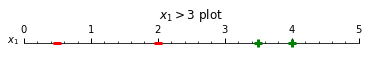
\includegraphics[width=70mm,scale=0.4]{images/classification_images/x1_1d_plot_points.png}

            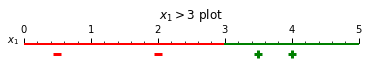
\includegraphics[width=70mm,scale=0.4]{images/classification_images/x1_1d_plot.png}
            
            \caption*{We plot everything above $x=3$ as \textbf{positive}, and \textbf{negative} otherwise.}
        \end{figure}
        
        We could also call it $\theta_0$, in the spirit of our $\theta$ notation for parameters.
        
        \begin{equation}
            x_1 + \theta_0 > 0
        \end{equation}
    
    \subsection{1-D classifiers in 2-D}
        
        Let's add a variable and see how our classifier looks on a 2-D plot.
            \note{We'll omit the data points for now.}
        
        \begin{figure}[H]
                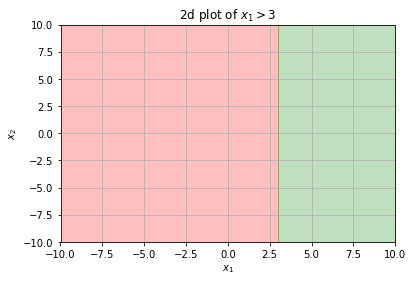
\includegraphics[width=70mm,scale=0.5]{images/classification_images/x1_2d_plot.png}
                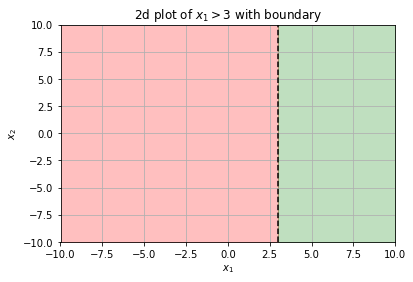
\includegraphics[width=70mm,scale=0.5]{images/classification_images/x1_2d_plot_boundary.png}
                
                \caption*{On the right, we've drawn the \textbf{dividing} line between our two regions.}
        \end{figure}
        
        Interesting - the \textbf{boundary} between positive and negative is defined by a \textbf{vertical line}.
        
        Or, almost. Compare $x_1>3$ and $x_1<3$:
        
        \begin{figure}[H]
                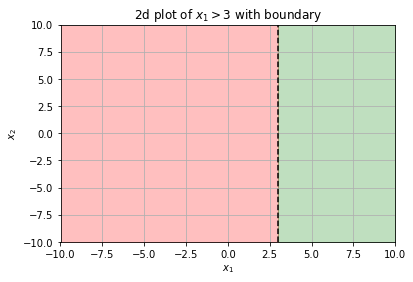
\includegraphics[width=70mm,scale=0.5]{images/classification_images/x1_2d_plot_boundary.png}
                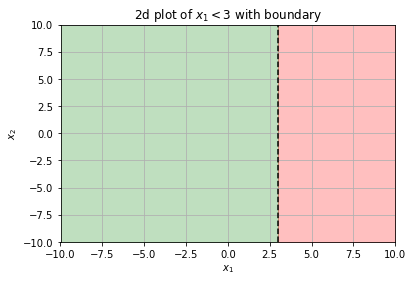
\includegraphics[width=70mm,scale=0.5]{images/classification_images/x1_2d_plot_boundary_reversed.png}
                
                \caption*{These two plots have the same line, but have their sides flipped.}
        \end{figure}
        
        So, we have a \textbf{line} that gives us the boundary, but we \textbf{also} need to include information about which way is the \textbf{positive} direction.
        
        What tool best represents \textbf{direction}? We could use angles, but we haven't used that much so far. Instead, let's use a \textbf{vector} to \textbf{point} in the right direction.
        
        \begin{figure}[H]
                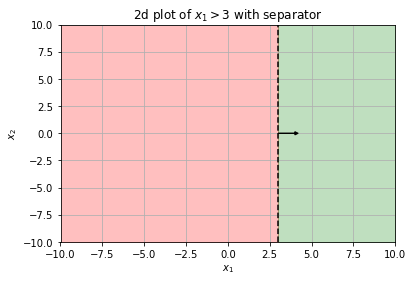
\includegraphics[width=70mm,scale=0.5]{images/classification_images/x1_2d_plot_separator.png}
                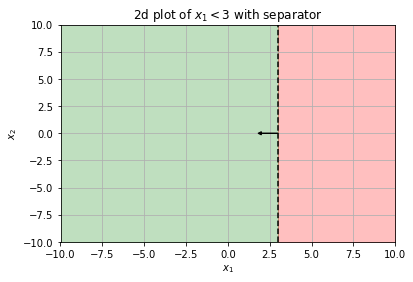
\includegraphics[width=70mm,scale=0.5]{images/classification_images/x1_2d_plot_separator_reversed.png}
                
                \caption*{Now, it's clear which plot is which, just using our \textbf{line} and \textbf{vector}!}
        \end{figure}
        
        The object that represents our classification is called a \textbf{separator}!
            \note{Since our variables are $x_1$ and $x_2$, this is a separator in \textbf{input space}.}\\
            
        \begin{definition}
            A \vocab{separator} defines how we \gren{separate} two different classes with our \purp{hypothesis}.
            
            It includes
            
            \begin{itemize}
                \item The \vocab{boundary}: the \gren{surface} where we \purp{switch} from one \purp{class} to another.
                \item The \vocab{orientation}: a \gren{description} of which \purp{side} of the boundary is assigned to \purp{which class}.
            \end{itemize}
        \end{definition}
        
        \note{We call it "orientation" because you could imagine "flipping over" the space, so the positive and negative regions are swapped.}
        
        For example, let's take our specific separator from above.\\
        
        \begin{concept}
            We can define our \vocab{1-D separator} using
            
            \begin{itemize}
                \item The \vocab{boundary} between the \gren{positive} and \redd{negative} regions: in 2-D input space, this looks like a vertical or horizontal \purp{line}.
                
                \item A \vocab{vector} pointing towards whichever side is given a \gren{${+1}$ value}.
            \end{itemize}
        \end{concept}
    
    \subsection{A second 1-D separator, and our problem}
        
        What if we use $x_2$ to \textbf{separate} our data?
        
        \begin{figure}[H]
                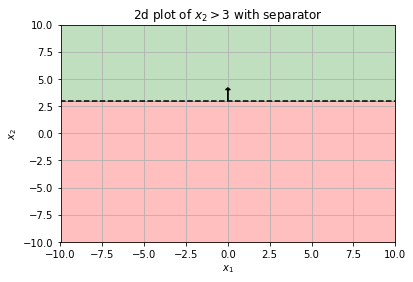
\includegraphics[width=70mm,scale=0.5]{images/classification_images/x2_2d_plot_separator.png}
                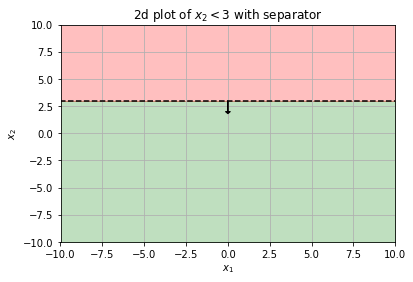
\includegraphics[width=70mm,scale=0.5]{images/classification_images/x2_2d_plot_separator_reversed.png}
                
                \caption*{Instead of having a vertical separator, we have a \textbf{horizontal} one.}
        \end{figure}
        
        We get the same sort of plot along the \textbf{other axis}!
        
        So, this is cool so far, but it's not a very \textbf{powerful} model: we can only handle a situation where the data is evenly divided by \textbf{one axis}.
        
        And if that's the case, what's the point of our \textbf{other} variable?
        
        \begin{figure}[H]
            \centering
                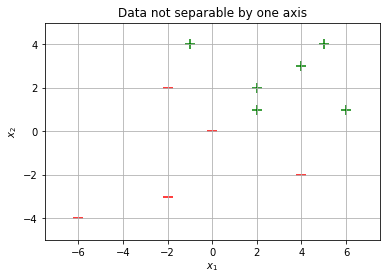
\includegraphics[width=70mm,scale=0.5]{images/classification_images/data_not_1d_separable.png}
                
                \caption*{There's no vertical or horizontal line we can use to split this space!}
        \end{figure}
        
    \subsection{The 2-D Separator: What vector do we use?}
    
        Just looking at our example, we might wonder, "well, if we can use \textbf{vertical} lines or \textbf{horizontal} lines, can't we just use a line in \textbf{another} orientation?
        
        It turns out, we \textbf{can}!
        
        \begin{figure}[H]
            \centering
                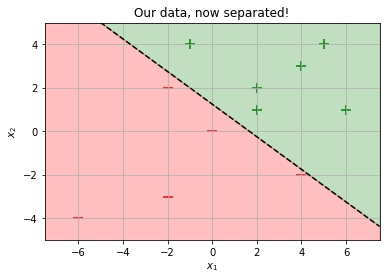
\includegraphics[width=70mm,scale=0.5]{images/classification_images/data_2d_separable.png}
                
                \caption*{If allow lines at an angle, we can classify all of our data correctly!}
        \end{figure}
        
        So, we've got our \textbf{boundary}. But we still need a vector to tell us which side is \textbf{positive}. But there are \textbf{many} possible vectors we could choose:
        
        \begin{figure}[H]
            \centering
                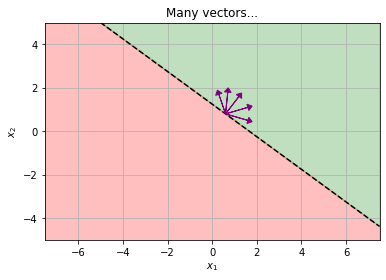
\includegraphics[width=70mm,scale=0.5]{images/classification_images/many_vectors_for_a_plane.png}
                
                \caption*{All of these vectors point towards the \textbf{correct} side of the plane. Is there a \textbf{best} one to use?}
        \end{figure}
        
        Above, we used the vector that was \textbf{vertical} or \textbf{horizontal}. This makes sense: if we're doing $x_1>3$, it seems reasonable to have the arrow \textbf{point} in the positive-$x_1$ direction.
        
        But this vector also happened to be \textbf{perpendicular} to our \textbf{line}: this is the line's \textbf{normal vector}, $\hat{n}$. This vector has a couple nice properties:
        
        \begin{itemize}
            \item It is \textbf{unique}: in 2-D, there is only 1 \textbf{normal} direction.
                \note{The opposite side is just $-\hat{n}$.}
                
            \item It points directly \textbf{away} from the plane.
            
            \item If our plane is at the \textbf{origin}, any point with a \textbf{positive} $\hat{n}$ component is on the \textbf{positive} side.
                \note{This will be important later!}
        \end{itemize}
        
        So, we have a \textbf{unique} vector that tells us which side is \textbf{positive}. Let's go with that!\\
        
        \begin{concept}
            Every \gren{line} in 2-D has a \vocab{unique normal vector} that can be used to \purp{define} the \gren{angle/direction} of the line.
            
            The \purp{direction} the vector is "facing" is also called the \vocab{orientation}.
        \end{concept}
        
        Our normal vector for the above separator:
        
        \begin{figure}[H]

                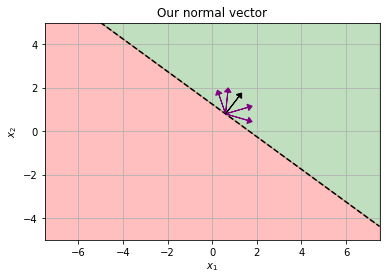
\includegraphics[width=70mm,scale=0.5]{images/classification_images/normal_vector_among_others.png}
                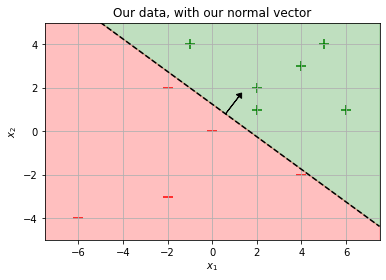
\includegraphics[width=70mm,scale=0.5]{images/classification_images/data_2d_separable_normal vector.png}
                
                \caption*{We can define our plane using the \textbf{normal} vector!}
        \end{figure}
        
        It's clear that this vector in some way is a \textbf{parameter}: if we change this vector, we get a different \textbf{orientation}, and a different \textbf{classifier}. 
        
        We have \textbf{represented} parameters in the past using $\theta$. We need \textbf{two} different $\theta_k$: one for the $x_1$ component, another for the $x_2$ component.
        
        So, we'll use that.\\
        
        \begin{notation}
            The vector $\theta$ represents the \vocab{normal vector} to our line in 2D.
            
            \begin{equation*}
                \hat{n} = \theta =
                \begin{bmatrix}
                        \theta_1 \\
                        \theta_2
                \end{bmatrix}
            \end{equation*}
        \end{notation}
        
        We add this to our diagram:
        
        \begin{figure}[H]
                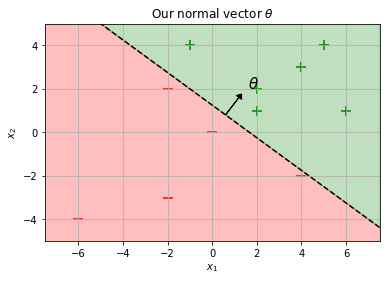
\includegraphics[width=70mm,scale=0.5]{images/classification_images/normal_vector_theta.png}
                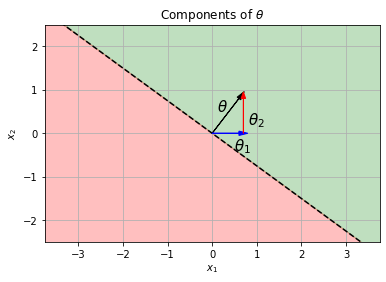
\includegraphics[width=70mm,scale=0.5]{images/classification_images/theta_components.png}
                
                \caption*{$\theta$ is our normal vector!}
        \end{figure}
        
        Nice work so far. The next question is: how do we describe this separator \textbf{mathematically}?
        
    \subsection{2D Separator - Matching components}
    
        As always, we'll \textbf{simplify} the problem to make it more manageable: for now, we'll assume our \textbf{separator} is centered at the \textbf{origin}.
        
        \begin{figure}[H]
            \centering
                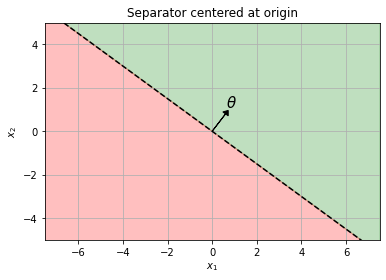
\includegraphics[width=70mm,scale=0.5]{images/classification_images/separator_centered_at_origin.png}
        \end{figure}
        
        So, we have our vector, $\hat{n}$. As we mentioned above, anything on the \textbf{same} side as $\hat{n}$ is \textbf{positive}, and anything on the \textbf{opposite} side is \textbf{negative}.
            \note{For a line on the origin, "On the same side of the line" can be interpreted as "has a positive $\hat{n}$ component". We'll find that component next.}\\
            
        \begin{figure}[H]
                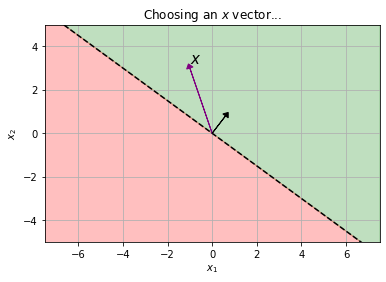
\includegraphics[width=70mm,scale=0.5]{images/classification_images/chose_a_vector.png}
                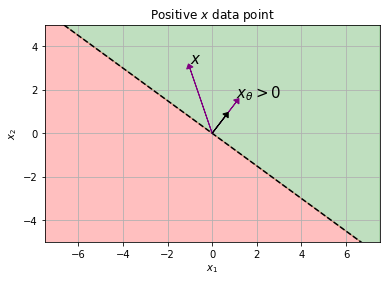
\includegraphics[width=70mm,scale=0.5]{images/classification_images/positive_v_vector.png}
                
                \caption*{This vector has a \textbf{positive} component in the $\theta$ direction.}
        \end{figure}
        
        \begin{figure}[H]
            \centering
                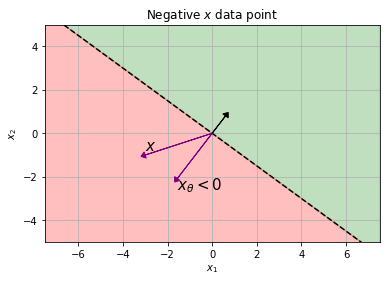
\includegraphics[width=70mm,scale=0.5]{images/classification_images/negative_v_vector.png}
                
                \caption*{This vector has a \textbf{negative} component in the $\theta$ direction.}
        \end{figure}
            
        How do we represent "on the same side" mathematically? How do we \textbf{find} whether the component is \textbf{positive} or \textbf{negative}? We use the \textbf{dot product}.\\
        
    \subsection{The Dot Product (Review)}
    
        How to calculate the dot product should be familiar to you, but we'll talk about some \textbf{intuition} that you may not be exposed to.\\
        
        \begin{concept}
            You can use the \vocab{dot product} between unit vectors to measure their "\purp{similarity}": if two vectors are more \gren{similar}, they have a \gren{larger} dot product.
            
            In the most clear cases, take unit vectors $\hat{a}$ and $\hat{b}$:
            
            \begin{itemize} 
                \item If they are in the \vocab{exact same} direction, $\hat{a} \cdot \hat{b} = 1$
                
                \item If they are in the \vocab{exact opposite} direction, $\hat{a} \cdot \hat{b} = -1$
                
                \item If they are \vocab{perpendicular} to each other, $\hat{a} \cdot \hat{b} = 0$
            \end{itemize}
        \end{concept}
        
            \note{Remember, \textbf{unit vectors} have a length of 1.}
        
        What about non-unit vectors?
        
        These unit vectors are then scaled up by the \textbf{magnitude} of each of our vectors. Because magnitudes are \textbf{always positive}, the dot product sign doesn't change.\\
        
        \begin{concept}
            You can use the \vocab{dot product} between non-unit vectors to measure their "similarity" \purp{scaled by their magnitude}. 
            
            If two vectors are more \gren{similar}, they have a \gren{larger} dot product. 
            
            \begin{itemize}
                \item If the vectors are \vocab{less} than $90^{\circ}$ apart, they are more similar: they will share a \textbf{positive} component: $\vec{a} \cdot \vec{b} > 0$
                
                \item If the vectors are \vocab{more} than $90^{\circ}$ apart, they will share a \textbf{negative} component: $\vec{a} \cdot \vec{b} < 0$
                
                \item If they are \vocab{perpendicular} ($90^{\circ}$) to each other, $\vec{a} \cdot \vec{b} = 0$
            \end{itemize}
        \end{concept}
        
    \subsection{Using the dot product}
        
        So, the \textbf{sign} of the dot product is a useful tool. If a point is on the line, it is \textbf{perpendicular} to $\theta$, our \textbf{normal vector}.
        
        So, if a point has a \textbf{positive} dot product, it is on the \textbf{same side} as $\theta$, and if it's \textbf{negative}, it's on the opposite side.
        
        \begin{figure}[H]
        
                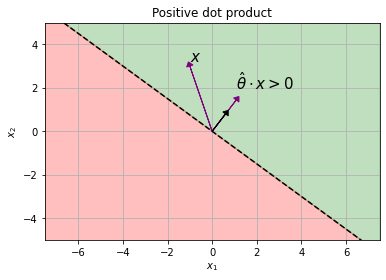
\includegraphics[width=45mm,scale=0.3]{images/classification_images/positive_v_vector_theta_hat.png}
                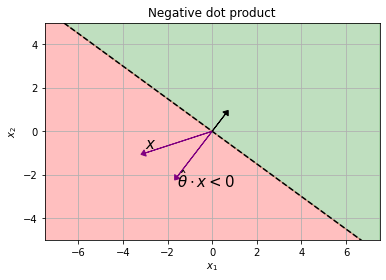
\includegraphics[width=45mm,scale=0.3]{images/classification_images/negative_v_vector_theta_hat.png}
                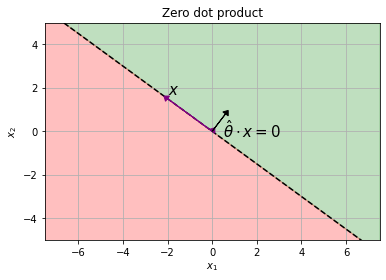
\includegraphics[width=45mm,scale=0.3]{images/classification_images/zero_v_vector_theta_hat.png}
                
                \caption*{Our various dot products can show us where in the space we are.}
        \end{figure}        
        
        So, we can classify things based on the \textbf{sign} of it. Written as an equation, we can define the sign function:\\
        
        \begin{kequation}
            For a \vocab{linear separator} centered on the \purp{origin}, we can do \vocab{binary classification} using the hypothesis
            
            \begin{equation*}
                h(x; \theta) = \text{sign}(\theta \cdot x )= 
                \begin{cases}
                    +1 & \text{if $\theta \cdot x > 0$} \\
                    -1 & \text{otherwise}
                \end{cases}
            \end{equation*}
        \end{kequation}
        
    \subsection{Introducing our offset}
        
        Now that we have handled the case where our linear separator is on the \textbf{origin}, we want to \textbf{shift} our separator \textbf{away} from it.
        
        In our \textbf{1-D} case, we easily \textbf{shifted} away from the origin: any separator $x_1>C$ where $C$ \textbf{isn't zero}, we shift by $C$ units.
        
        \begin{figure}[H]
            \centering
                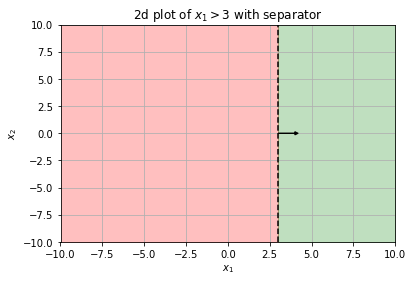
\includegraphics[width=70mm,scale=0.5]{images/classification_images/x1_2d_plot_separator.png}
                \caption*{By making our inequality $x_1>3$ \textbf{nonzero}, we moved away from the origin by 3 units!}
        \end{figure}
        
        We could make our inequality \textbf{nonzero}, then! That could move us \textbf{away} from the origin, just in a different \textbf{direction}.
        
        Or, we could equivalently do this...
            \note{Note: $A \Longleftrightarrow B$ means $A$ and $B$ are equivalent!}
        
        \begin{equation}
            x_1 >3 \Longleftrightarrow x_1-3 > 0
        \end{equation}
        
        So, instead, we could just add a constant to our expression, which we will call $\theta_0$.
        
        We'll also switch out $\theta \cdot x = \theta^T x$.\\
        
        \begin{kequation}
            A general \vocab{linear separator} can do \vocab{binary classification} using the hypothesis
            
            \begin{equation*}
                h(x; \theta) = \text{sign}(\theta^T x + \theta_0 )= 
                \begin{cases}
                    +1 & \text{if $\theta^T x + \theta_0 > 0$} \\
                    -1 & \text{otherwise}
                \end{cases}
            \end{equation*}
        \end{kequation}
        
        Notice that this looks very similar to what we did in regression! We'll get into that in a bit.
        
        First, a quick look at the components of our equation:\\
        
        \begin{concept}
            For \vocab{binary classification}, $\theta$ and $\theta_0$ entirely \purp{define} our \vocab{linear separator}.
            
            \begin{itemize}
                \item $\theta$ gives us the \purp{orientation} of our line.
                \item $\theta_0$ \purp{shifts} that line around in \gren{space}.
            \end{itemize}
        \end{concept}
    
    \subsection{How does the offset affect our classifier?}
    
        So, how exactly does our offset $\theta_0$ affect our \textbf{classifier}? Well, we mark our classifier with our \textbf{normal vector} and the \textbf{boundary}.
        
        Our \textbf{normal vector} is entirely captured by $\theta$: it's unchanged by $\theta_0$.
        
        What about our \textbf{boundary}? We have its \textbf{orientation}, but we don't know where it has \textbf{shifted} to.
        
        \begin{figure}[H]
            \centering
                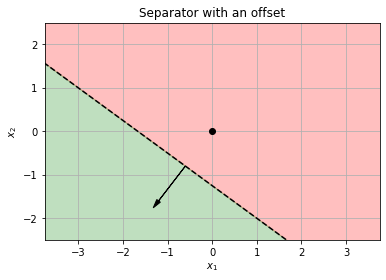
\includegraphics[width=70mm,scale=0.5]{images/classification_images/separator_with_offset.png}
                \caption*{Note that the origin has been marked.}
        \end{figure}
        
        Well, let's use our equation: the \textbf{boundary} line is given by 
        
        \begin{equation}
            \theta^T x + \theta_0 = 0 
            \Longleftrightarrow 
            \theta^T x = -\theta_0
        \end{equation}
        
        We'll break the effects of $\theta_0$ into three cases:
            \note{Note: the below statements are true no matter what $\theta$ we choose!}
        
        For each, we'll show two different $\theta$ values.
        
        \begin{itemize}
            \item If $\theta_0=0$, then $x=(0,0)$ is \textbf{on the line}.
                \begin{itemize}
                    \item Without an \textbf{offset}, our line goes through the \textbf{origin}.
                \end{itemize}
                
                \begin{figure}[H]
                    \centering                         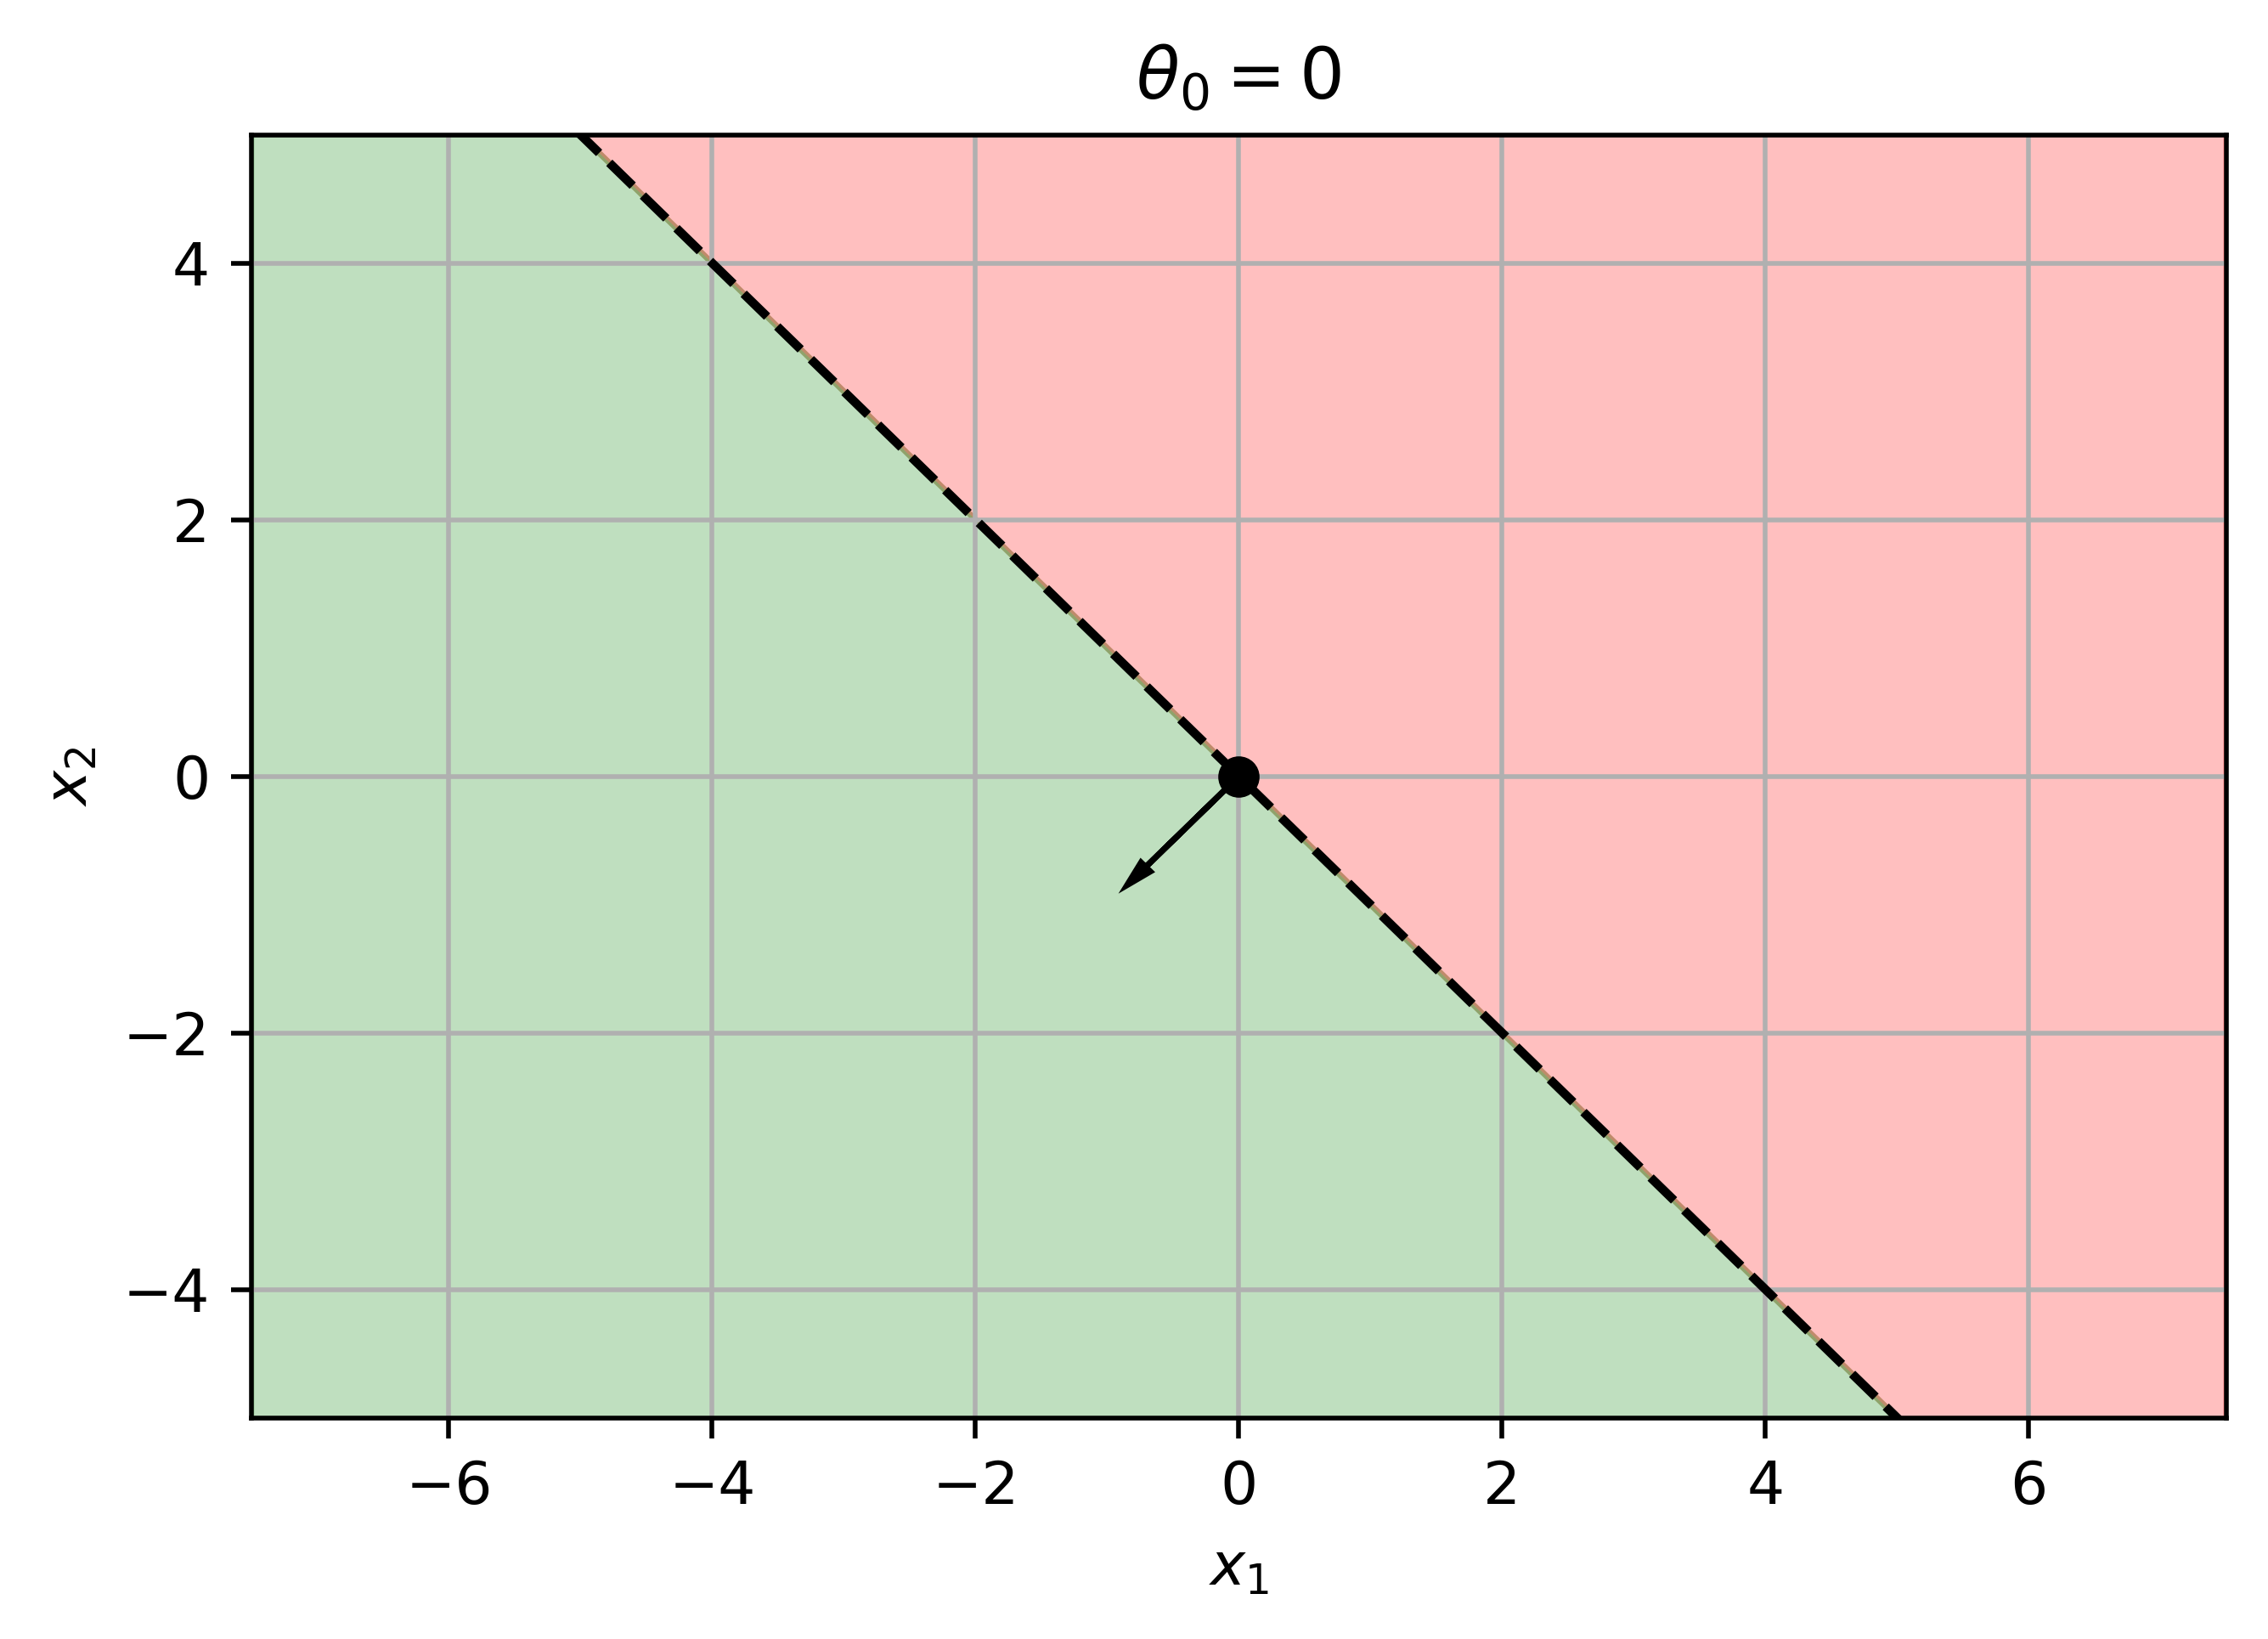
\includegraphics[width=60mm,scale=0.5]{images/classification_images/theta_0_zero.png}
                    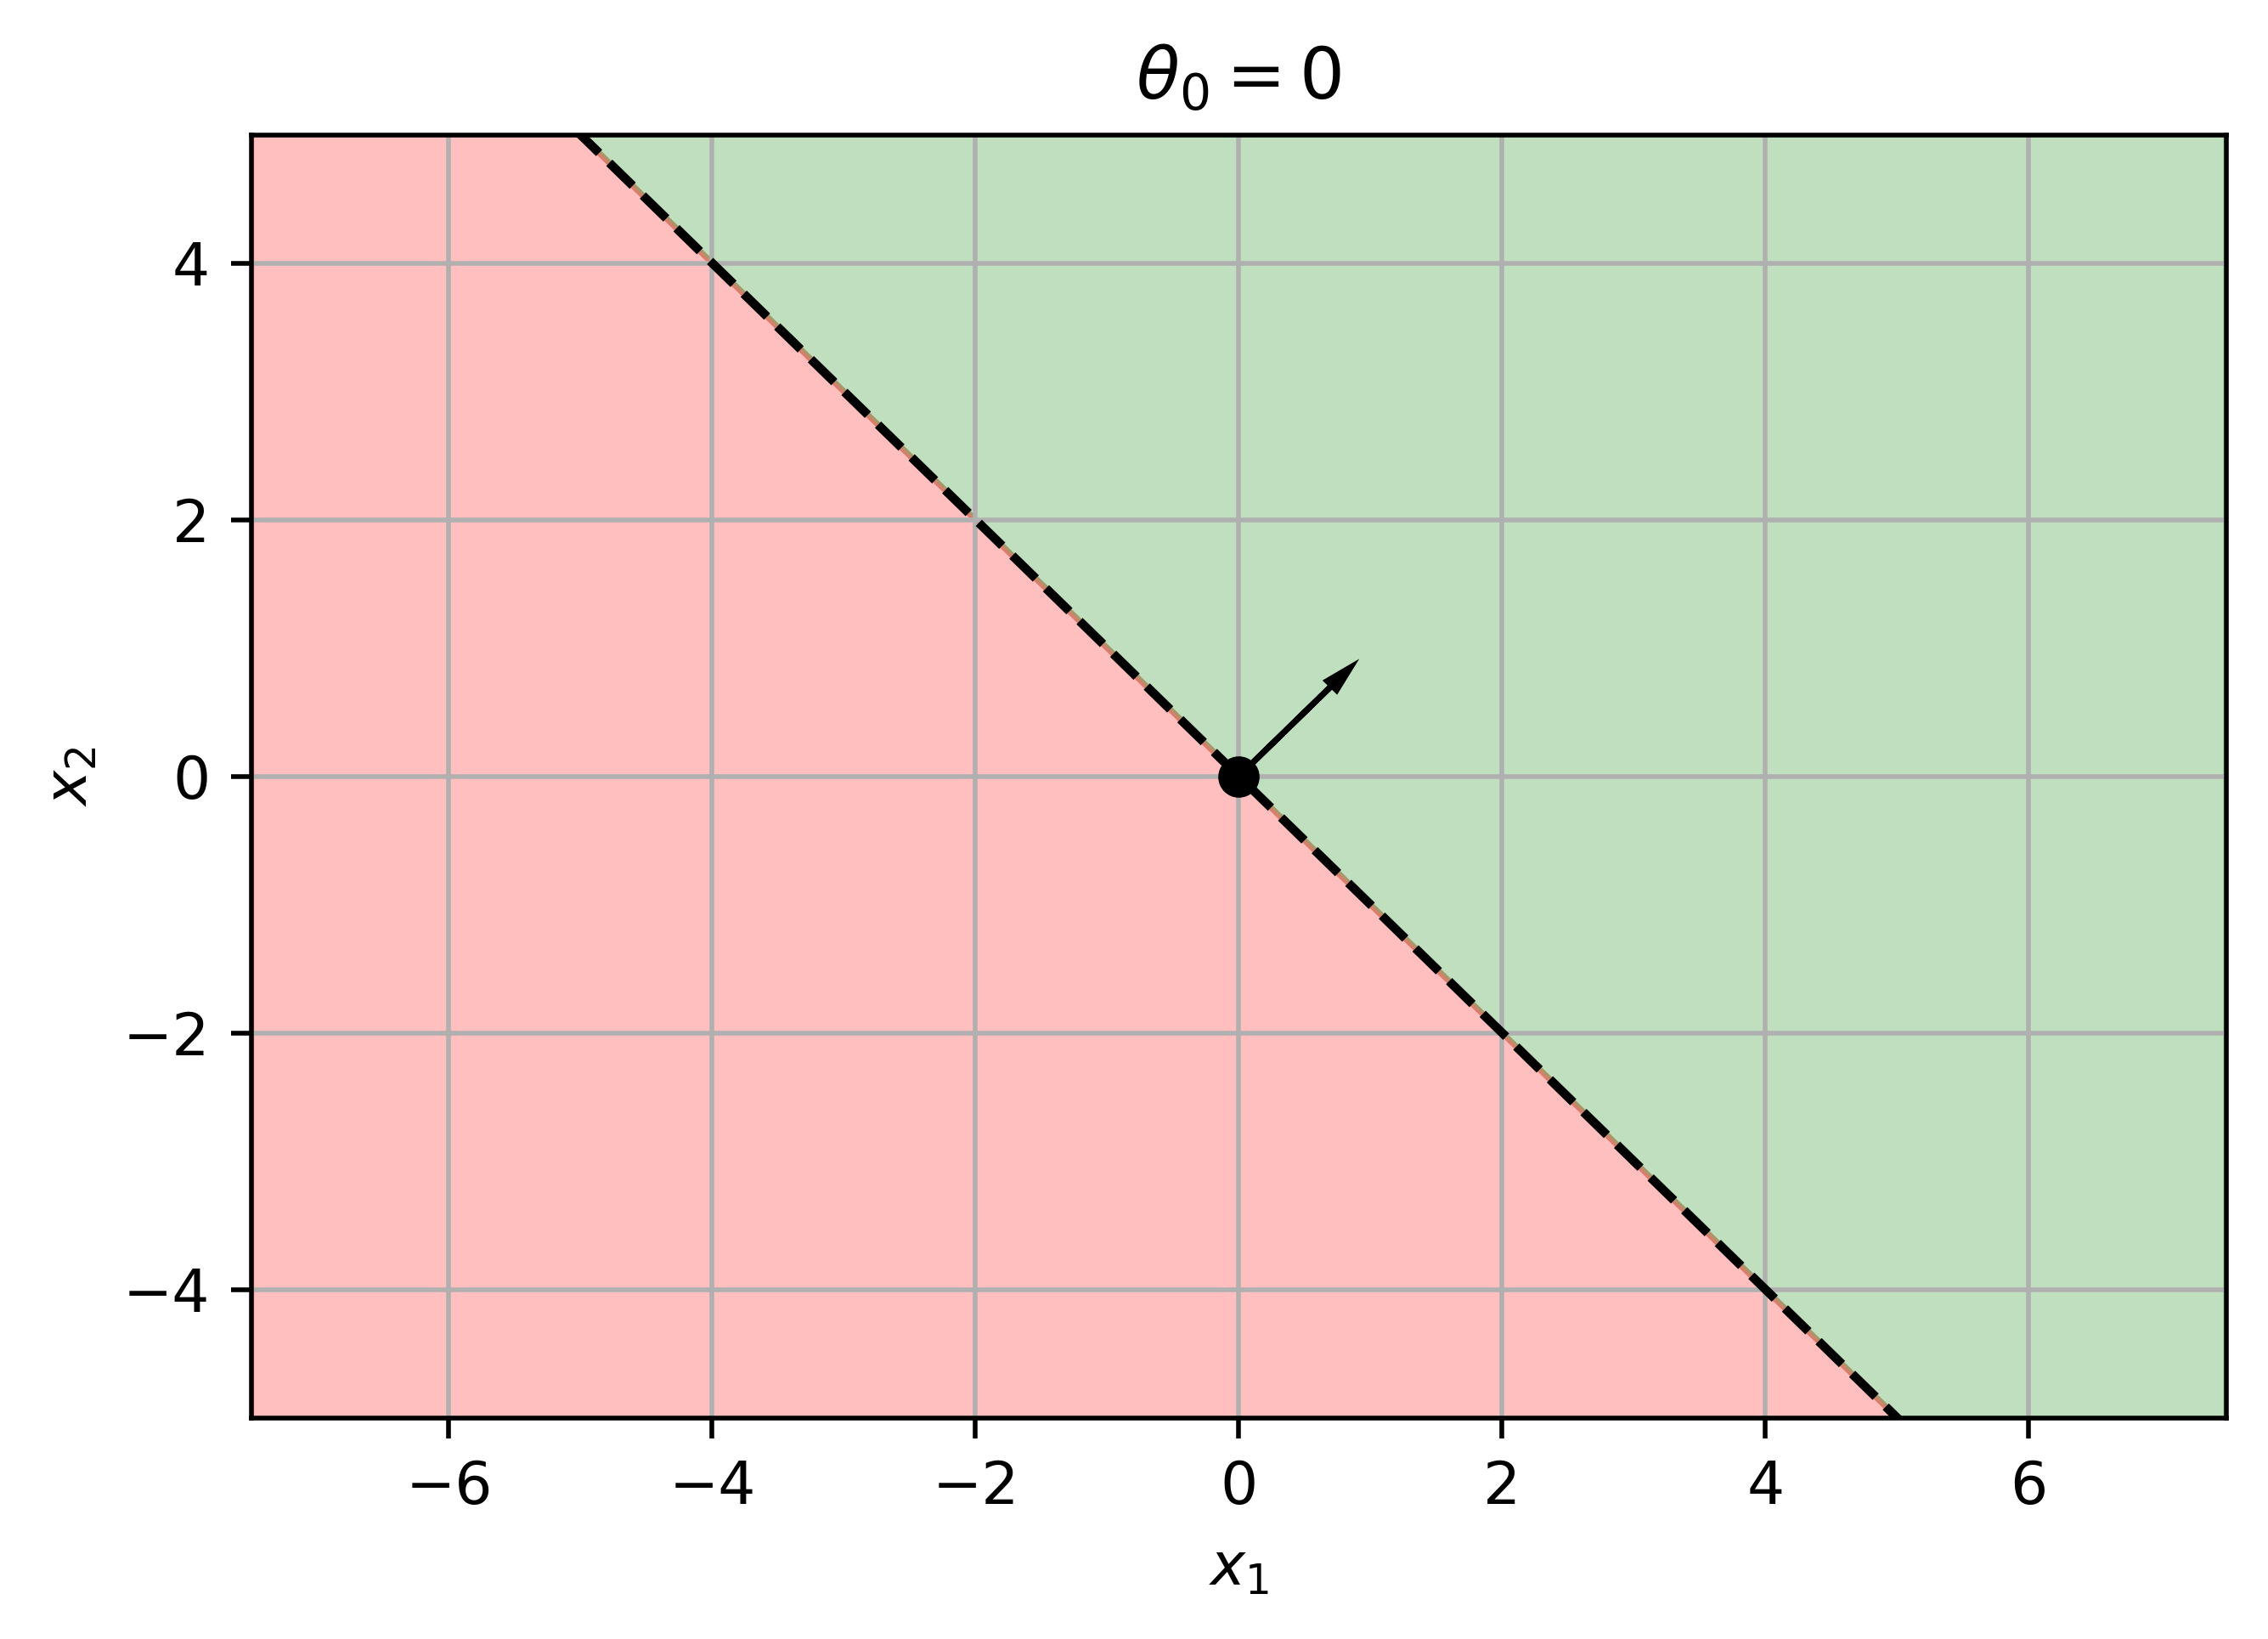
\includegraphics[width=60mm,scale=0.5]{images/classification_images/zero_theta0_positive_theta.png}
                        \caption*{The boundary is on the origin.}
                \end{figure}
                
            \item If $\theta_0>0$, then $x=(0,0)$ is in the \textbf{positive} region.
                \begin{itemize}
                    \item That means the positive region is \textbf{larger}: the line must have moved in the $-\theta$ direction.
                \end{itemize}
                
                \begin{figure}[H]
                    \centering                         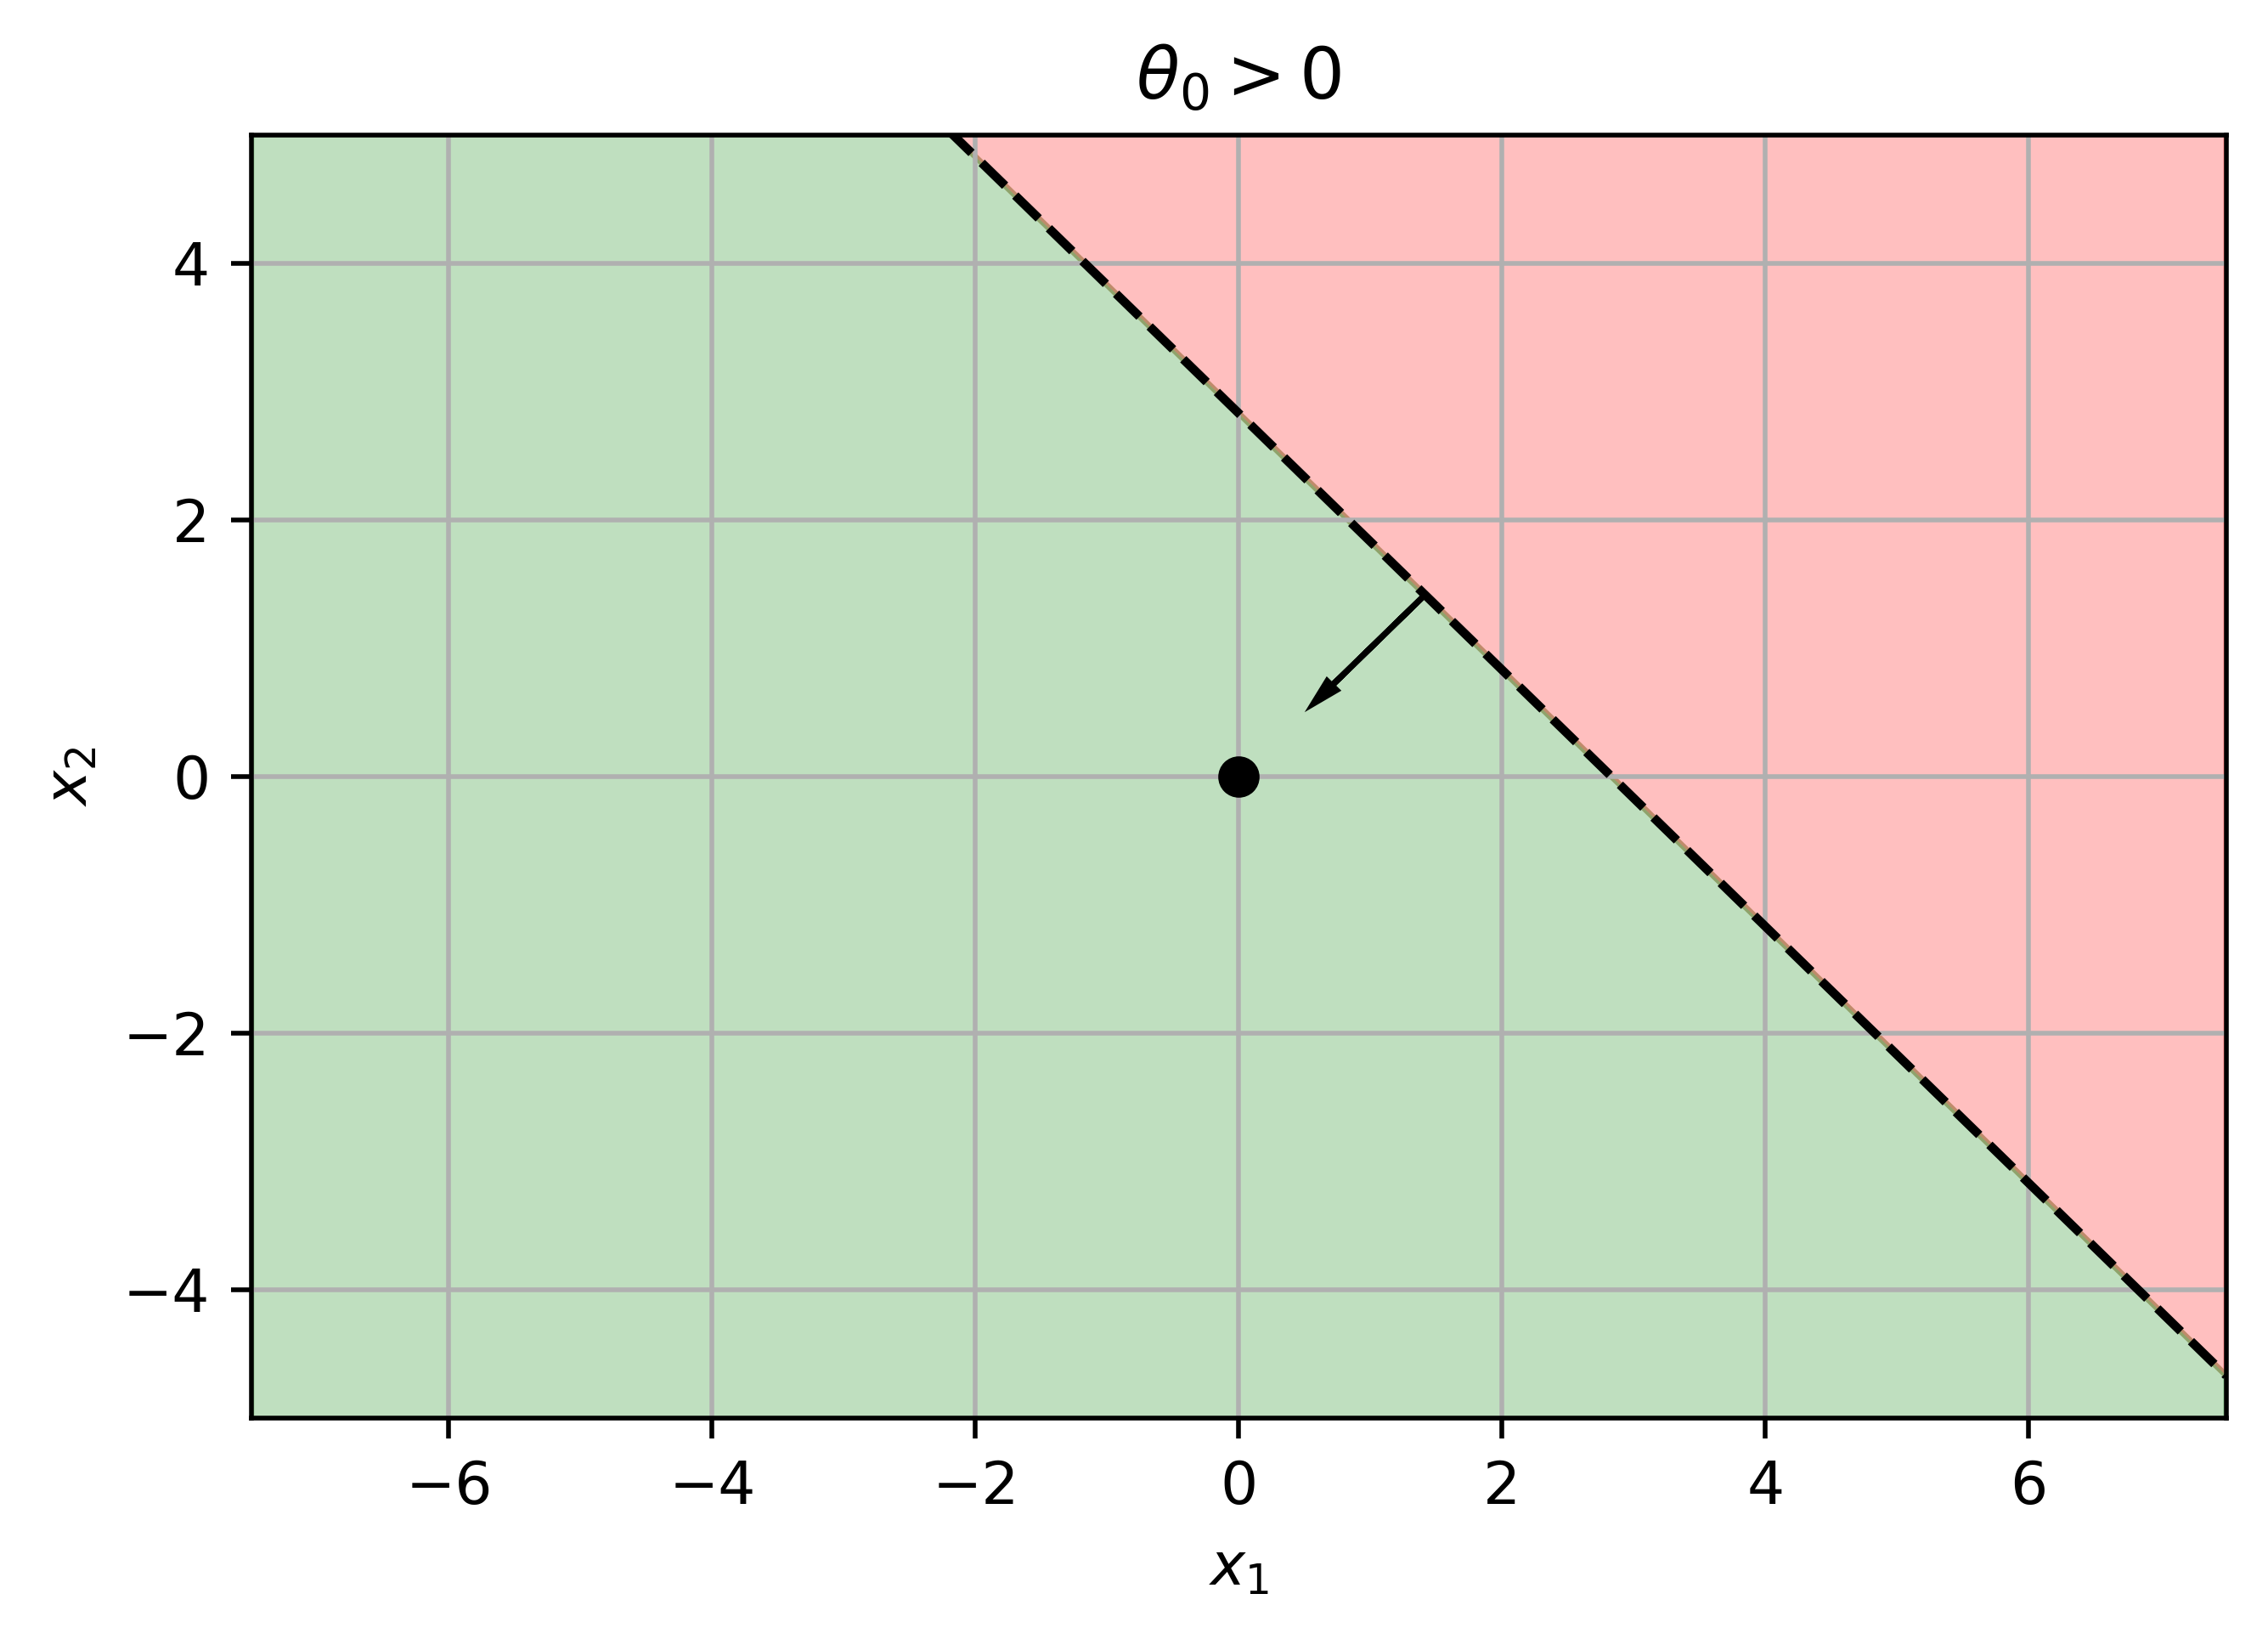
\includegraphics[width=60mm,scale=0.5]{images/classification_images/theta_0_greater_zero.png}
                    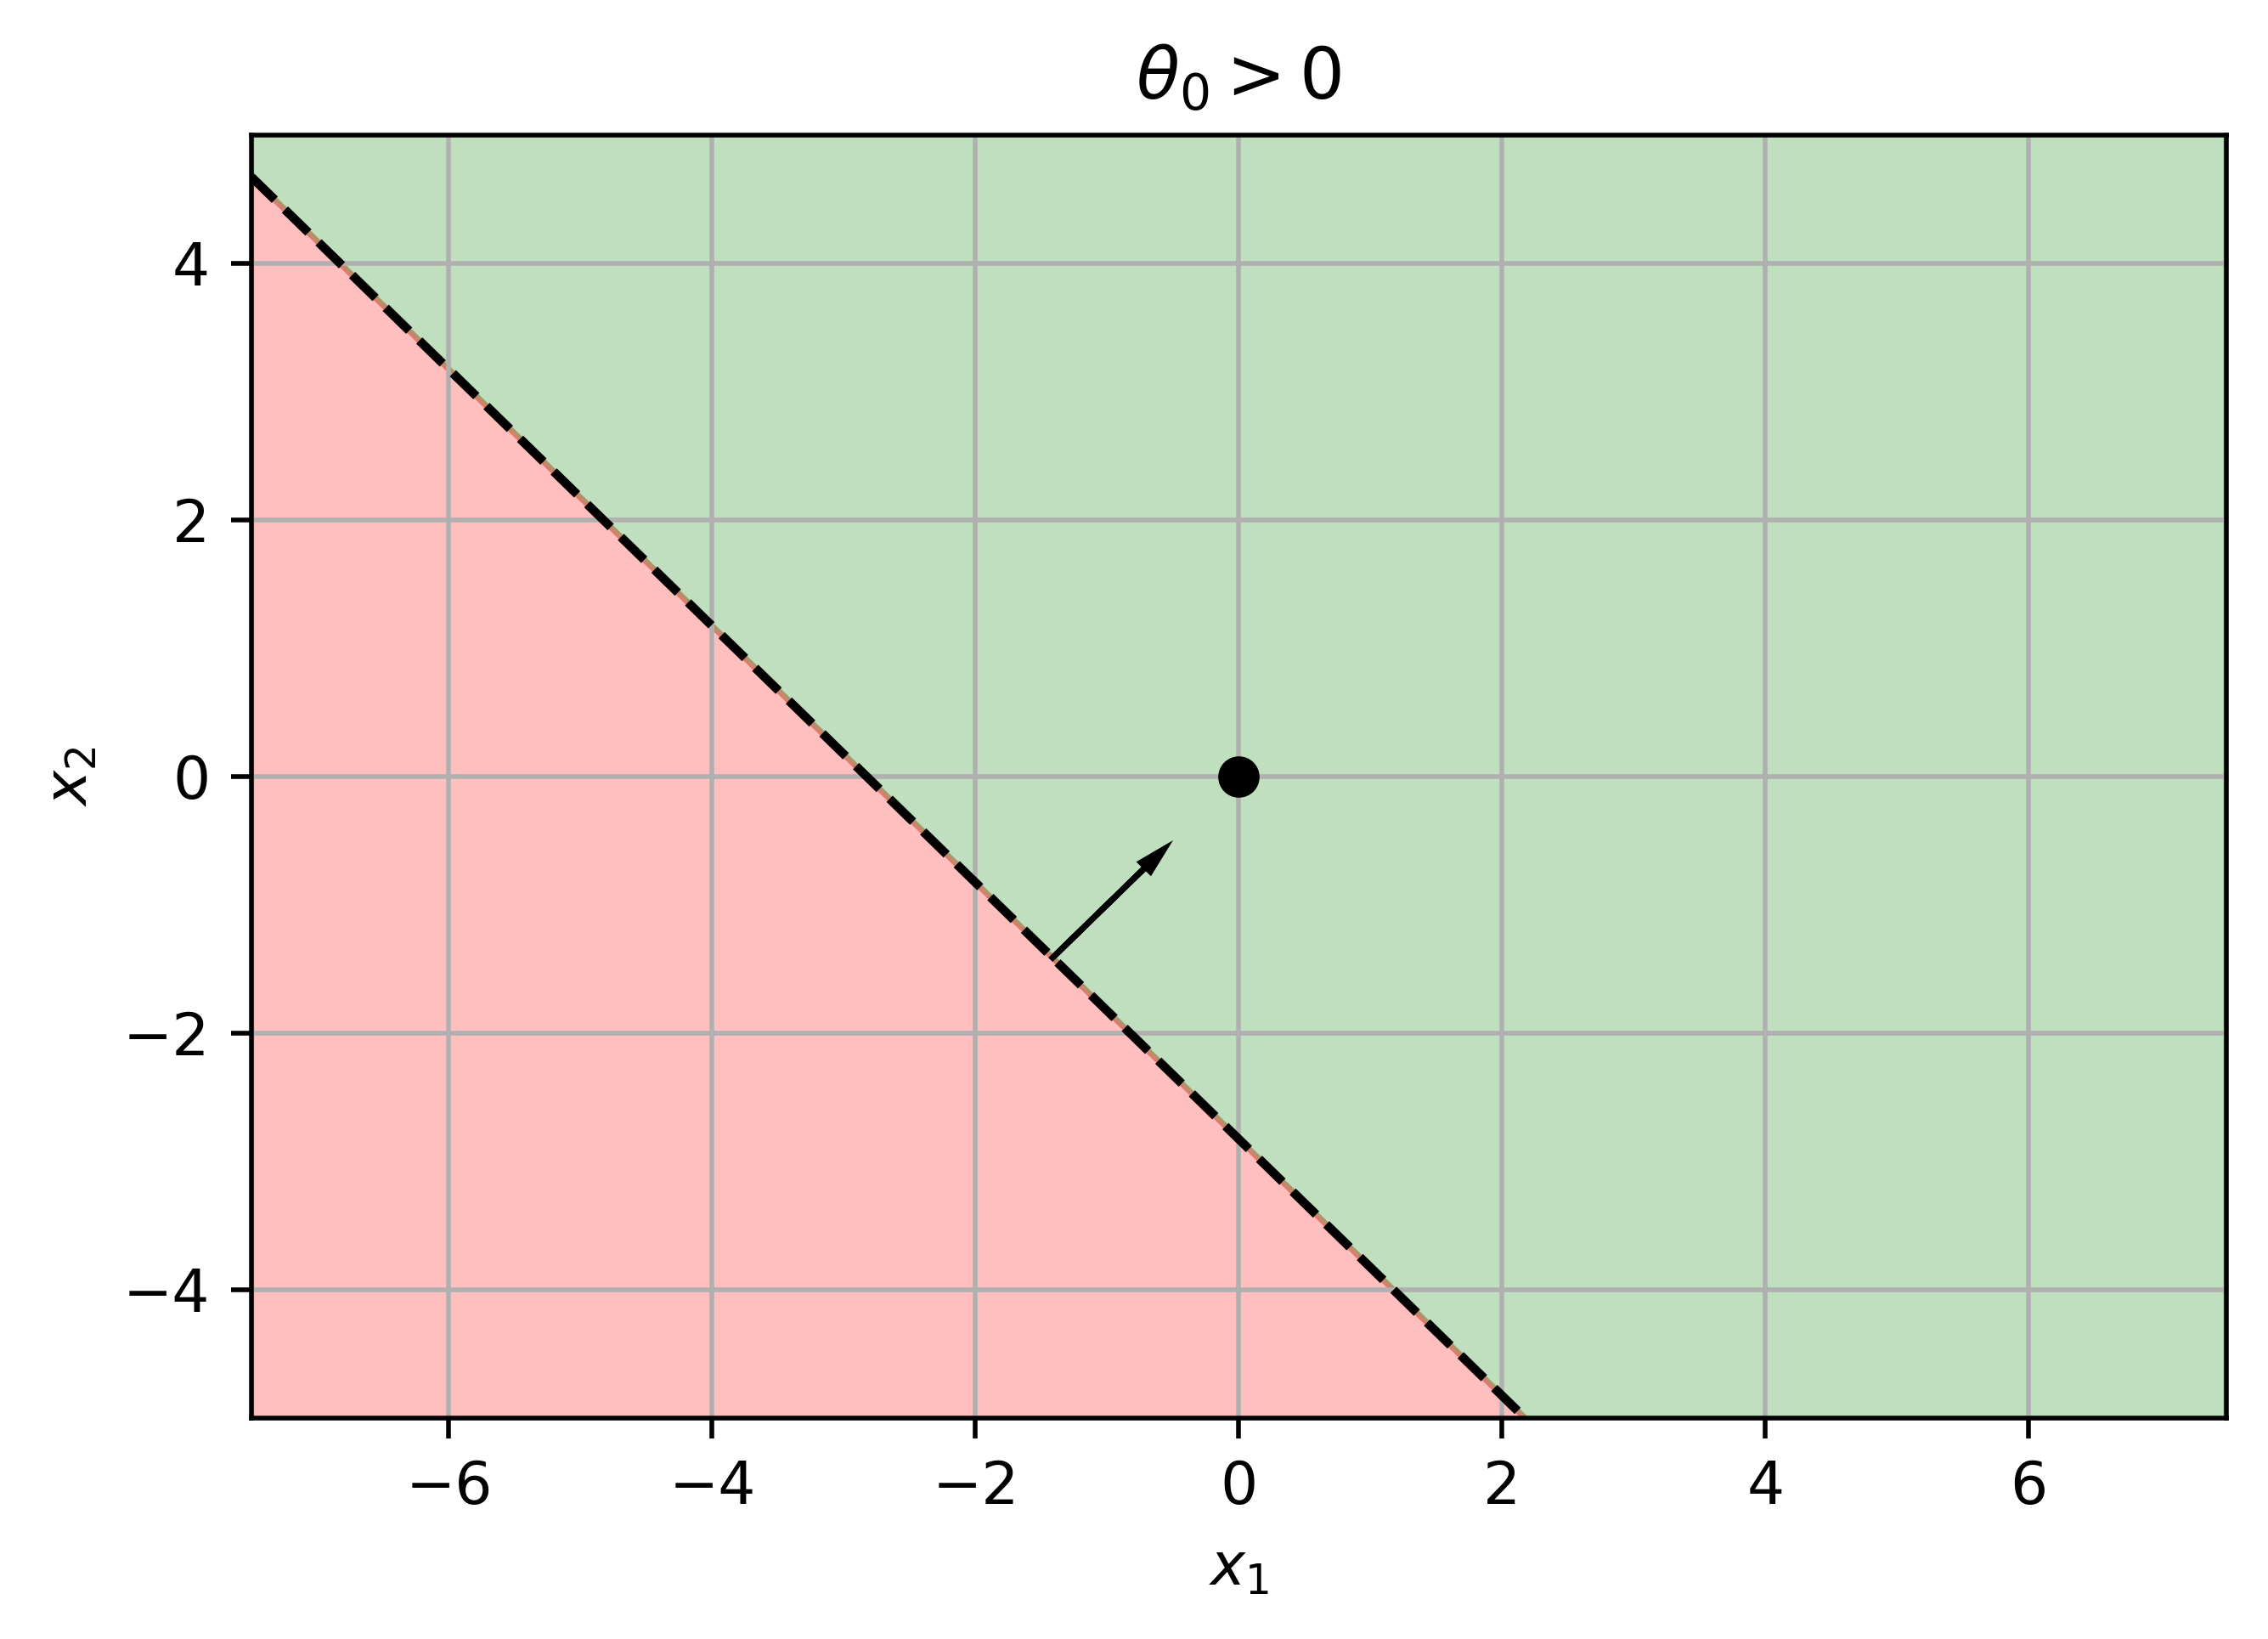
\includegraphics[width=60mm,scale=0.5]{images/classification_images/positive_theta0_positive_theta.png}
                        \caption*{If we have a \textbf{positive} constant, it's "easier" to get a positive \textbf{result}: more positive space.}
                \end{figure}
                
                
            \item If $\theta_0<0$, then $x=(0,0)$ is in the \textbf{negative} region.
                \begin{itemize}
                    \item That means the positive region is \textbf{smaller}: the line must have moved in the $+\theta$ direction.
                \end{itemize}
                
                \begin{figure}[H]
                    \centering                         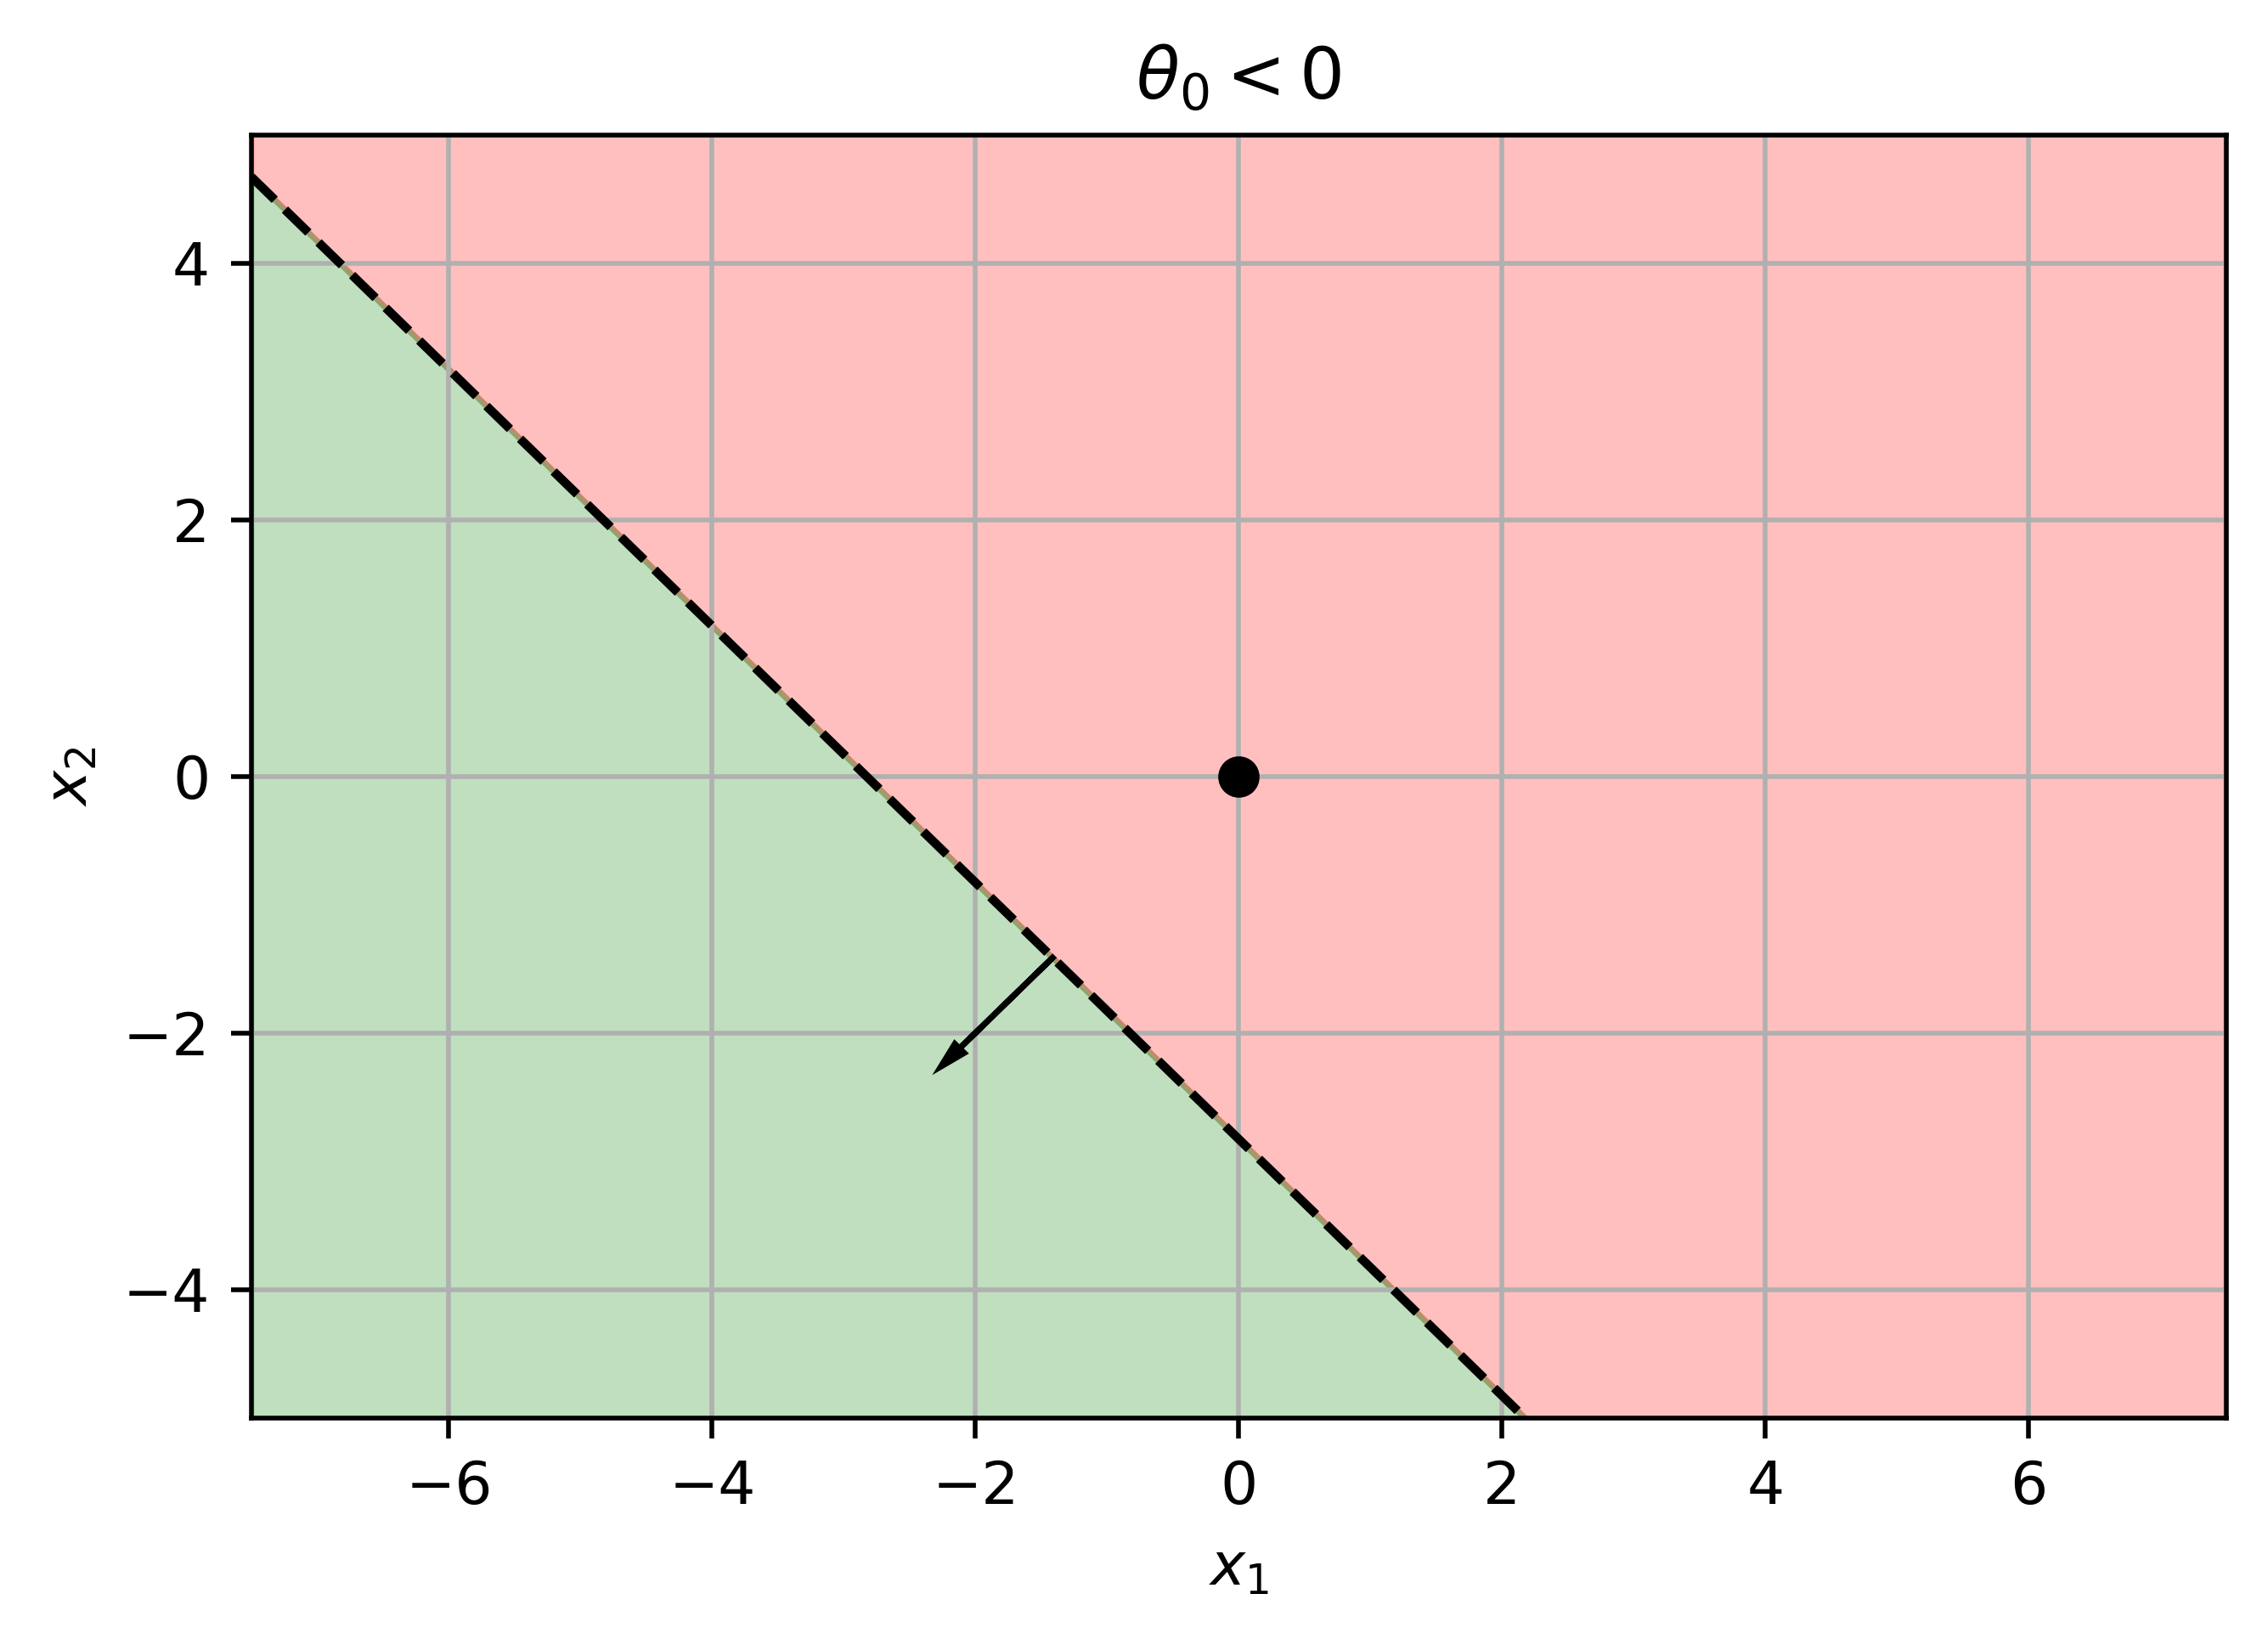
\includegraphics[width=60mm,scale=0.5]{images/classification_images/theta_0_less_zero.png}
                    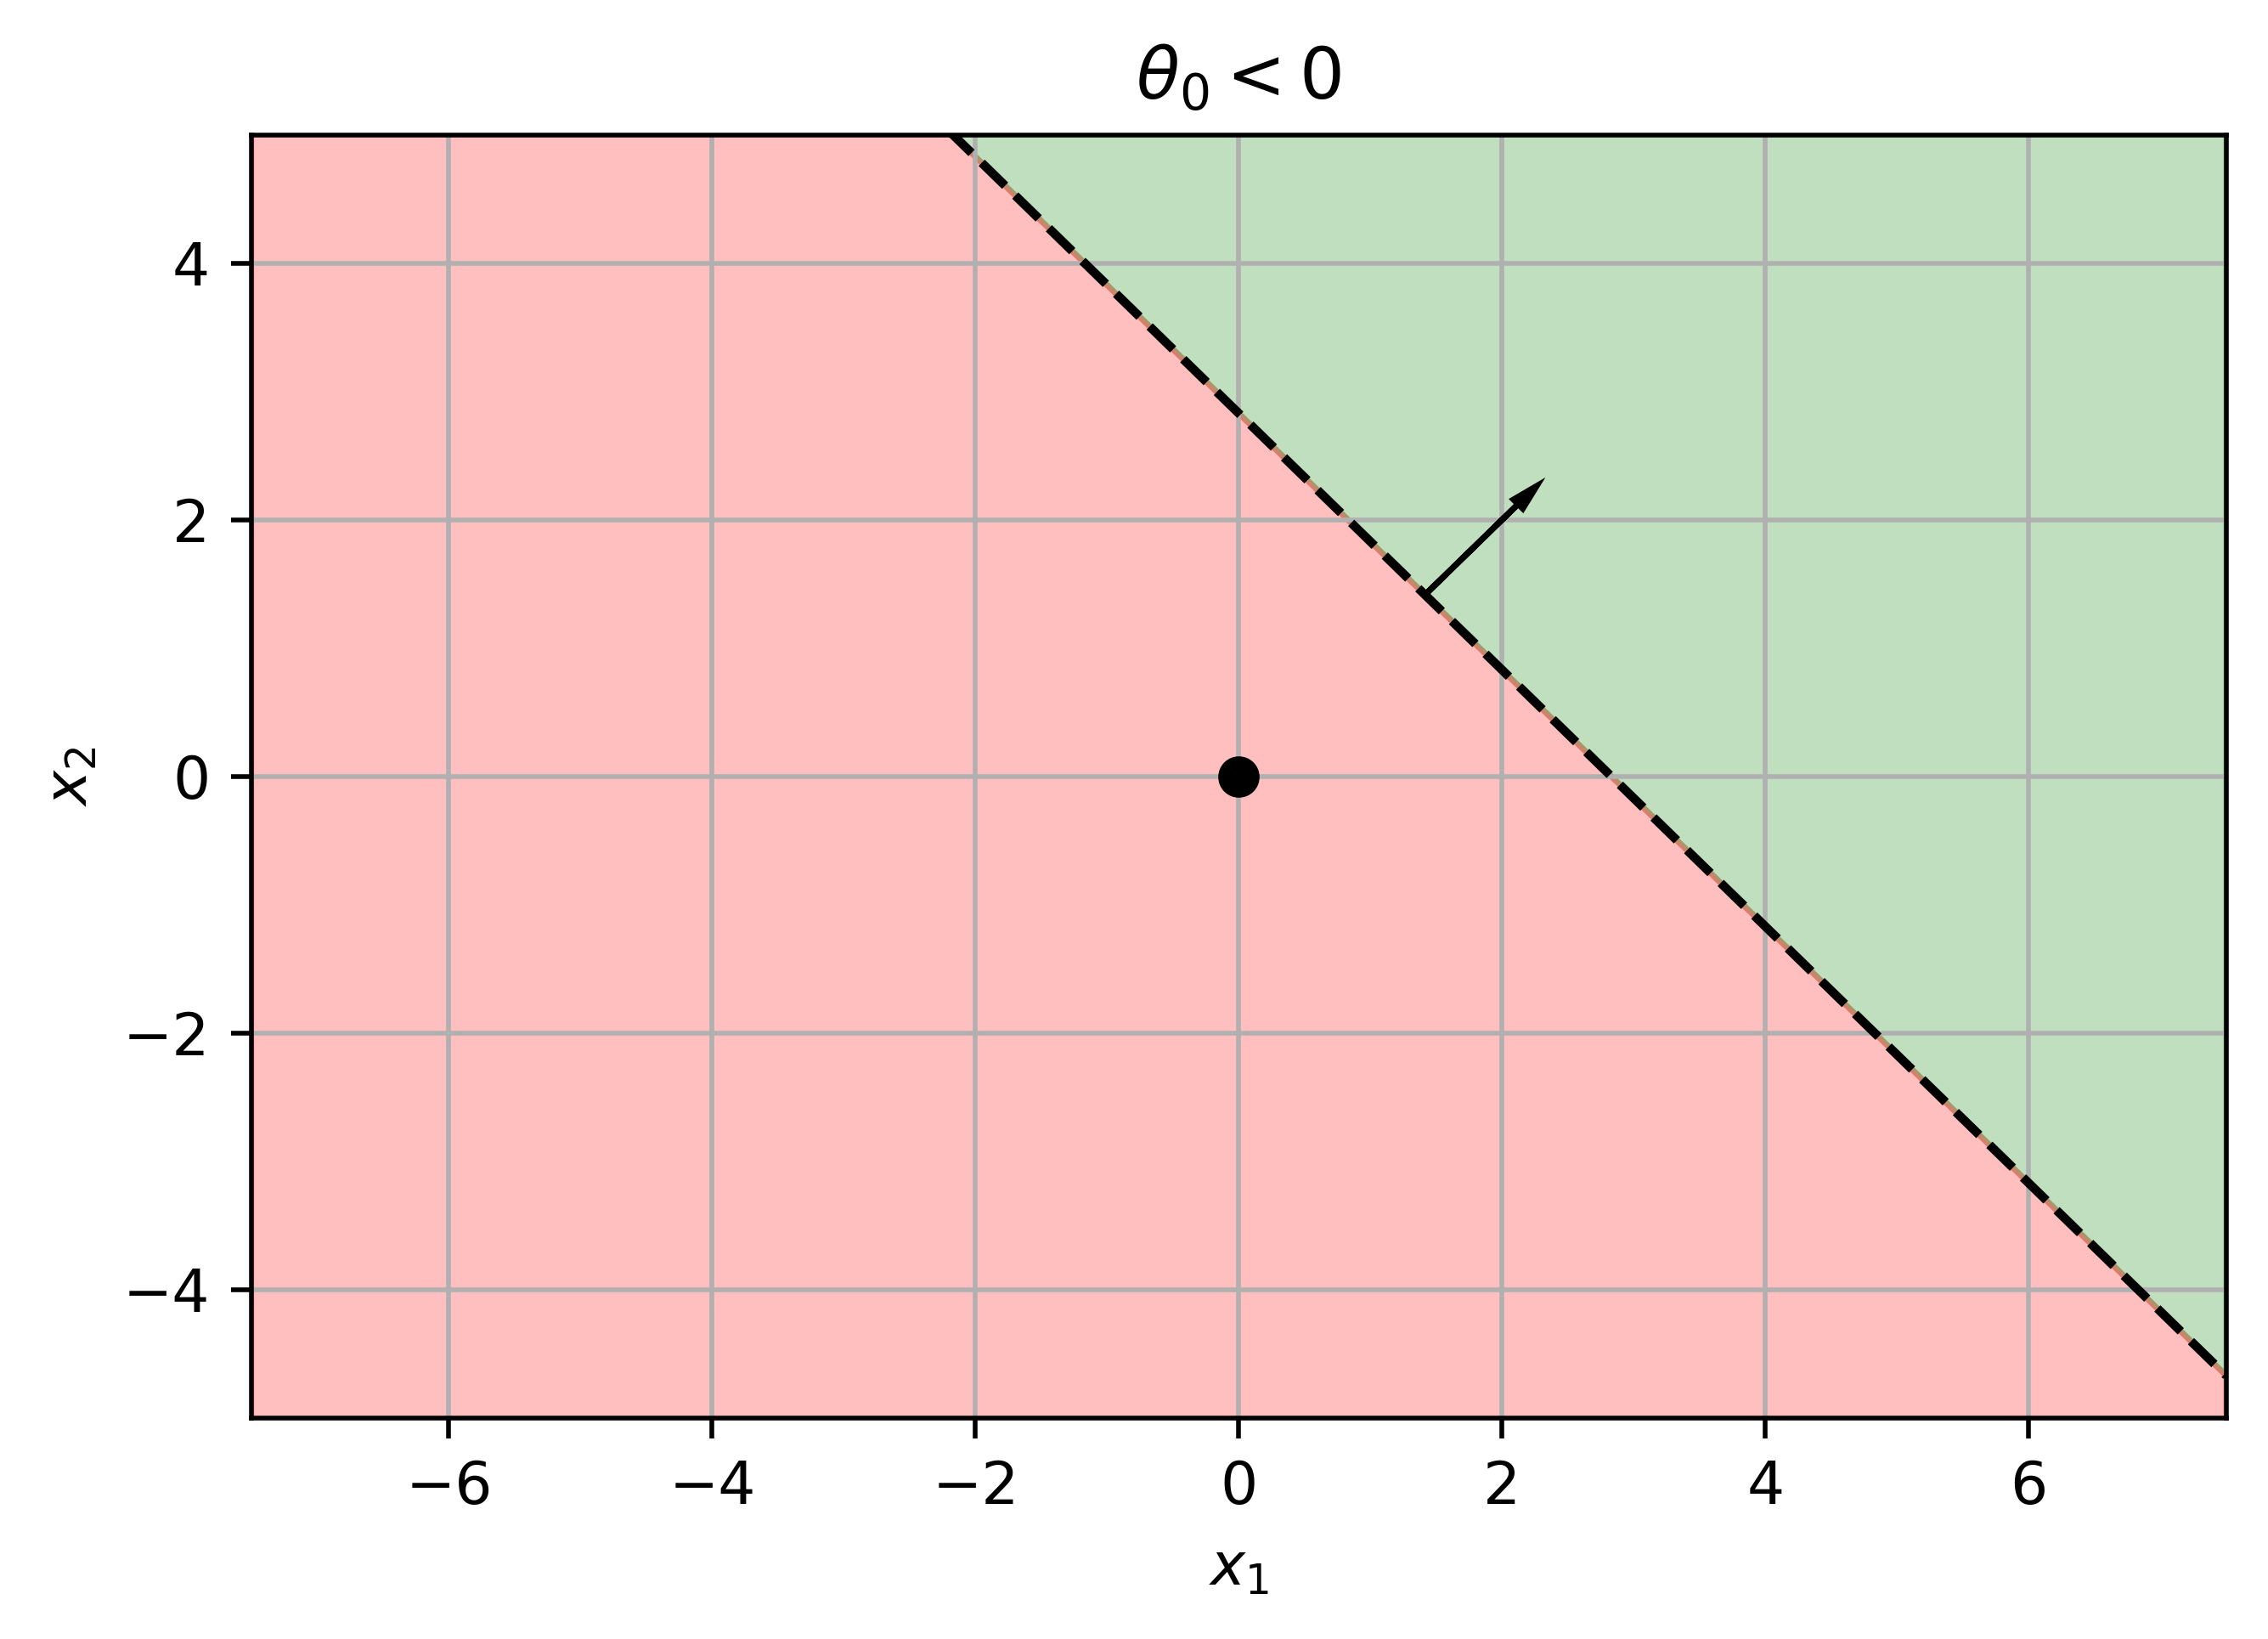
\includegraphics[width=60mm,scale=0.5]{images/classification_images/negative_theta0_positive_theta.png}
                        \caption*{If we have a \textbf{negative} constant, it's "harder" to get a positive \textbf{result}: more negative space.}
                \end{figure}
        \end{itemize}
        
        This can be a bit confusing, so we'll summarize:\\
        
            \begin{concept}
                The \gren{sign} of our $\theta_0$ and the \purp{direction} we move away from the origin are \vocab{opposite}.
                
                If \blu{$\theta_0>0$} (positive), our boundary moves in the \purp{$-\theta$ direction}.
                
                If \blu{$\theta_0<0$} (negative), our boundary moves in the \purp{$+\theta$ direction}.
            \end{concept}
        
        This gives us a general idea of how the offset affects it, but what is the \textbf{exact} effect of $\theta_0$ on the line?
        
        We'll focus on one point on the line: the \textbf{closest point to the origin} We want to look at this \textbf{point} because it's \textbf{unique}.
            \note{Points that aren't unique are hard to keep track of!}
    
    \subsection{Distance from the Origin to the Plane}
    
        \begin{figure}[H]
            \centering
                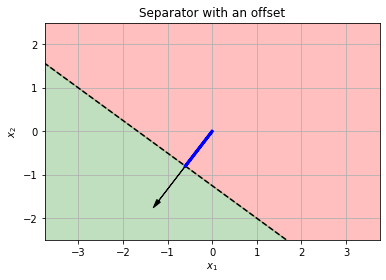
\includegraphics[width=70mm,scale=0.5]{images/classification_images/separator_with_offset_shown.png}
                \caption*{Notice that the \textbf{shortest} path from the origin to the line is \textbf{parallel} to $\theta$!}
        \end{figure}
        
        So, we can think of our \textbf{line} as having been \textbf{pushed} in the $\theta$ direction. This \textbf{matches} what we did for 1-D separators: $x_1>3$ was moved in the $x_1$ direction.
        
        So, we'll take the closest point on the line, $\vec{d}$. The \textbf{magnitude} $d$ will give us the \textbf{distance} that the separator has been \textbf{shifted}.
        
        \begin{figure}[H]
            \centering
                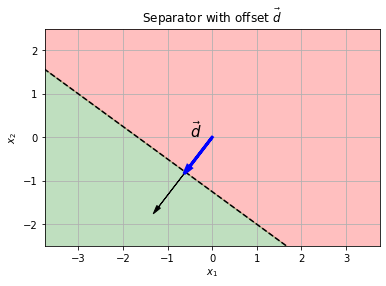
\includegraphics[width=70mm,scale=0.5]{images/classification_images/separator_with_offset_d.png}
        \end{figure}
        
        Since $\vec{d}$ is in the direction of $\theta$, the direction can be captured by the unit vector $\hat{\theta}$. Let's take a look at that:
            \note{Remember, a vector is direction (unit vector) times magnitude (scalar).}
            
        \begin{equation}
            \theta = \norm{\theta} \red{\hat{\theta}}
        \end{equation}
        
        \begin{equation}
            \vec{d} = d \red{\hat{\theta}}
        \end{equation}
        
        They're in the same \textbf{direction}, so they have the same \textbf{unit vector} $\hat{\theta}$.
        
        $\vec{d}$ is on the \textbf{line}, so it satisfies:
            \note{We'll use $\theta \cdot \vec{d}$ instead of $\theta^T \vec{d}$ here.}
        
        \begin{equation}
            \theta \cdot \vec{d} + \theta_0=0
        \end{equation}
        
        We can plug our equations 4.8 and 4.9, where we've separated magnitude from unit vector:
        
        \begin{equation}
        \overbrace{
            \Big(
                \norm{\theta} 
                \red{\hat{\theta}}
            \Big)
        }^{\theta}
        \cdot
        \overbrace{
            \Big(
            d \red{\hat{\theta}}
            \Big)
        }^{\vec{d}}
            + \theta_0
        \end{equation}
        
        We can move the scalars $\norm{\theta}$ and $d$ out of the way of the dot product:
        
        \begin{equation}
            \norm{\theta} d \left( 
                                \red{\hat{\theta} \cdot \hat{\theta}} 
                          \right) 
                          + \theta_0
        \end{equation}
        
        We know that $\hat{u} \cdot \hat{u}=1$:
        
        \begin{equation}
            \norm{\theta}d+\theta_0=0
        \end{equation}
        
        And now, we just solve for $d$:\\
        
        \begin{concept}
            The \vocab{distance} $d$ from the \purp{origin} to our \gren{linear separator} is 
            
            \begin{equation}
                d = \frac{ -\theta_0}{\norm{\theta}}
            \end{equation}
        \end{concept}
        
        A "negative" distance means $\vec{d}$ (the vector from the origin to the line) is pointed in the opposite direction of $\theta$.
        
        \begin{figure}[H]
            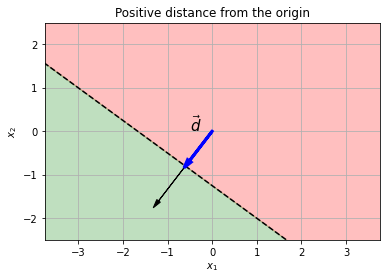
\includegraphics[width=70mm,scale=0.5]{images/classification_images/positive_distance.png}
            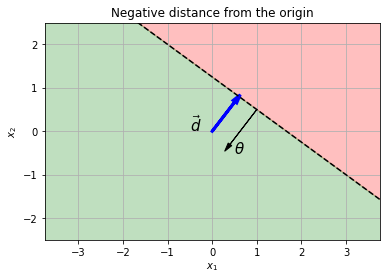
\includegraphics[width=70mm,scale=0.5]{images/classification_images/negative_distance.png}
            
        \end{figure}
        
        Notice, again, that this agrees with our \textbf{earlier} thought: the sign of $\theta_0$ is the opposite ($-1$) of the $\theta$ direction we move in.
        
    \subsection{Extending to higher dimensions}
    
        We've now fully conquered the 2D problem! Now, we can move up in \textbf{dimensions}.
        
        In terms of equations, the answer is simple, just like it is for regression: just add more terms to $\theta$.\\
        
        \begin{kequation}
            A general d-dimensional \vocab{linear separator} can do \vocab{binary classification} using the hypothesis
            
            \begin{equation*}
                h(x; \theta) = \text{sign}(\theta^T x + \theta_0 )= 
                \begin{cases}
                    +1 & \text{if $\theta^T x + \theta_0 > 0$} \\
                    -1 & \text{otherwise}
                \end{cases}
            \end{equation*}
            
            Where
            
            \begin{equation*}
                \theta = 
                \begin{bmatrix}
                  \theta_1 \\ \theta_2 \\ \vdots \\ \theta_d
                \end{bmatrix}
            \end{equation*}
        \end{kequation}
        
        What about how it looks? Well, if we have 3 input variables, our line turns into a \textbf{plane}:
        
        \begin{figure}[H]
            \centering
            
            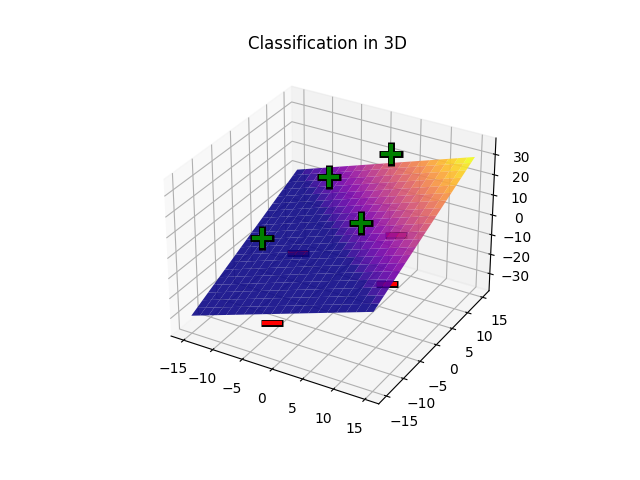
\includegraphics[width=70mm,scale=0.5]{images/classification_images/3d_classification_problem.png}

            \caption*{As we move into 3D, we can \textbf{separate} points on \textbf{three different axes}.}
        \end{figure}
        
        Just like with regression, this is when we introduce the \textbf{hyperplane}:\\
        
        \begin{concept}
            Our $n$-dimensional \vocab{linear separator} solution to the \vocab{binary classification} problem \purp{splits} our space into two \gren{halves}: a positive and a negative half.
            
            The \gren{surface} that \purp{splits} space like this is a $(n-1)$-dimensional \vocab{hyperplane}.
            
            The hyperplane is \vocab{oriented}: there is a \purp{normal} vector $\theta$ which defines the \purp{orientation} of the hyperplane, and which side is \gren{positive}.
            
            It also has an \gren{offset} term $\theta_0$, that slides it in the $\theta$ direction \purp{away} from the origin.
        \end{concept}
        
        For any dimensional input, we can use hyperplanes as separators.
        
    
    \subsection{IMPORTANT: A difference between regression and classification}
    
        Here is an important misconception that comes up between regression and classification.
        
        Both functions use the equation
        
        \begin{equation}
            \theta^T x + \theta_0
        \end{equation}
        
        So, one might think of them as interchangeable.
        
        However, they are \redd{not}. Why is that?
        
        \begin{figure}[H]

            
            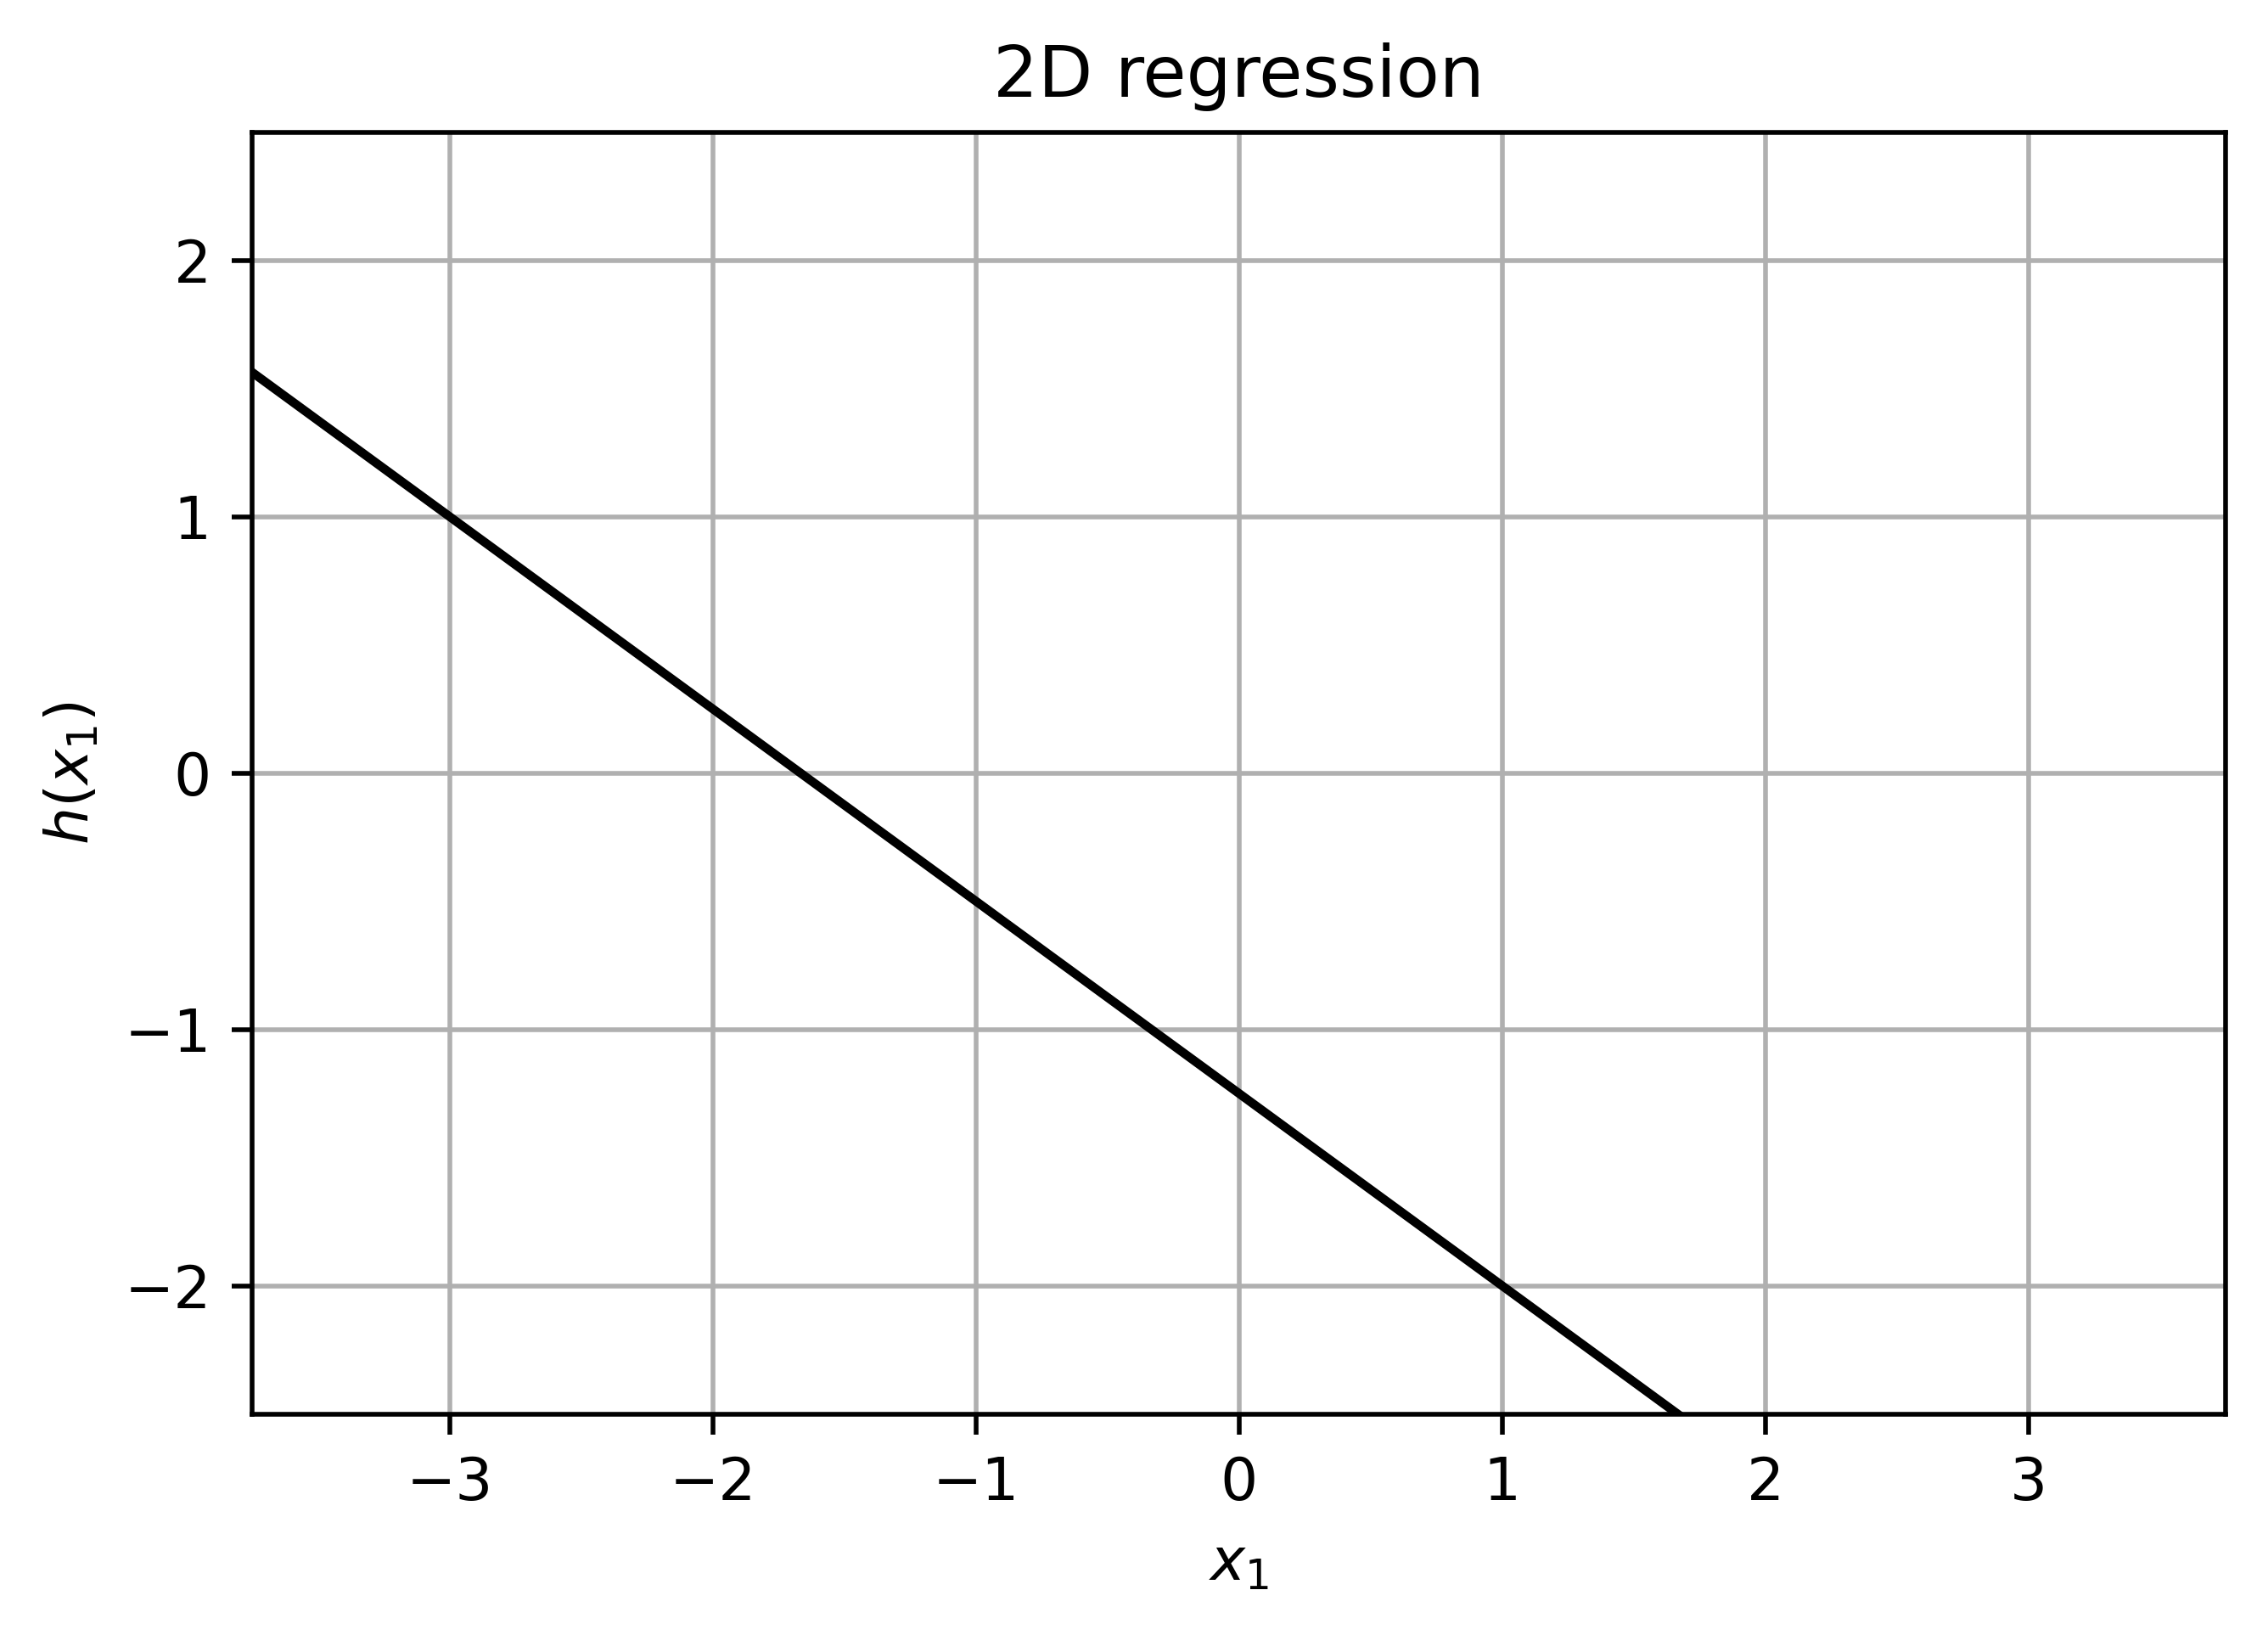
\includegraphics[width=70mm,scale=0.5]{images/classification_images/2d_regression_versus.png}
            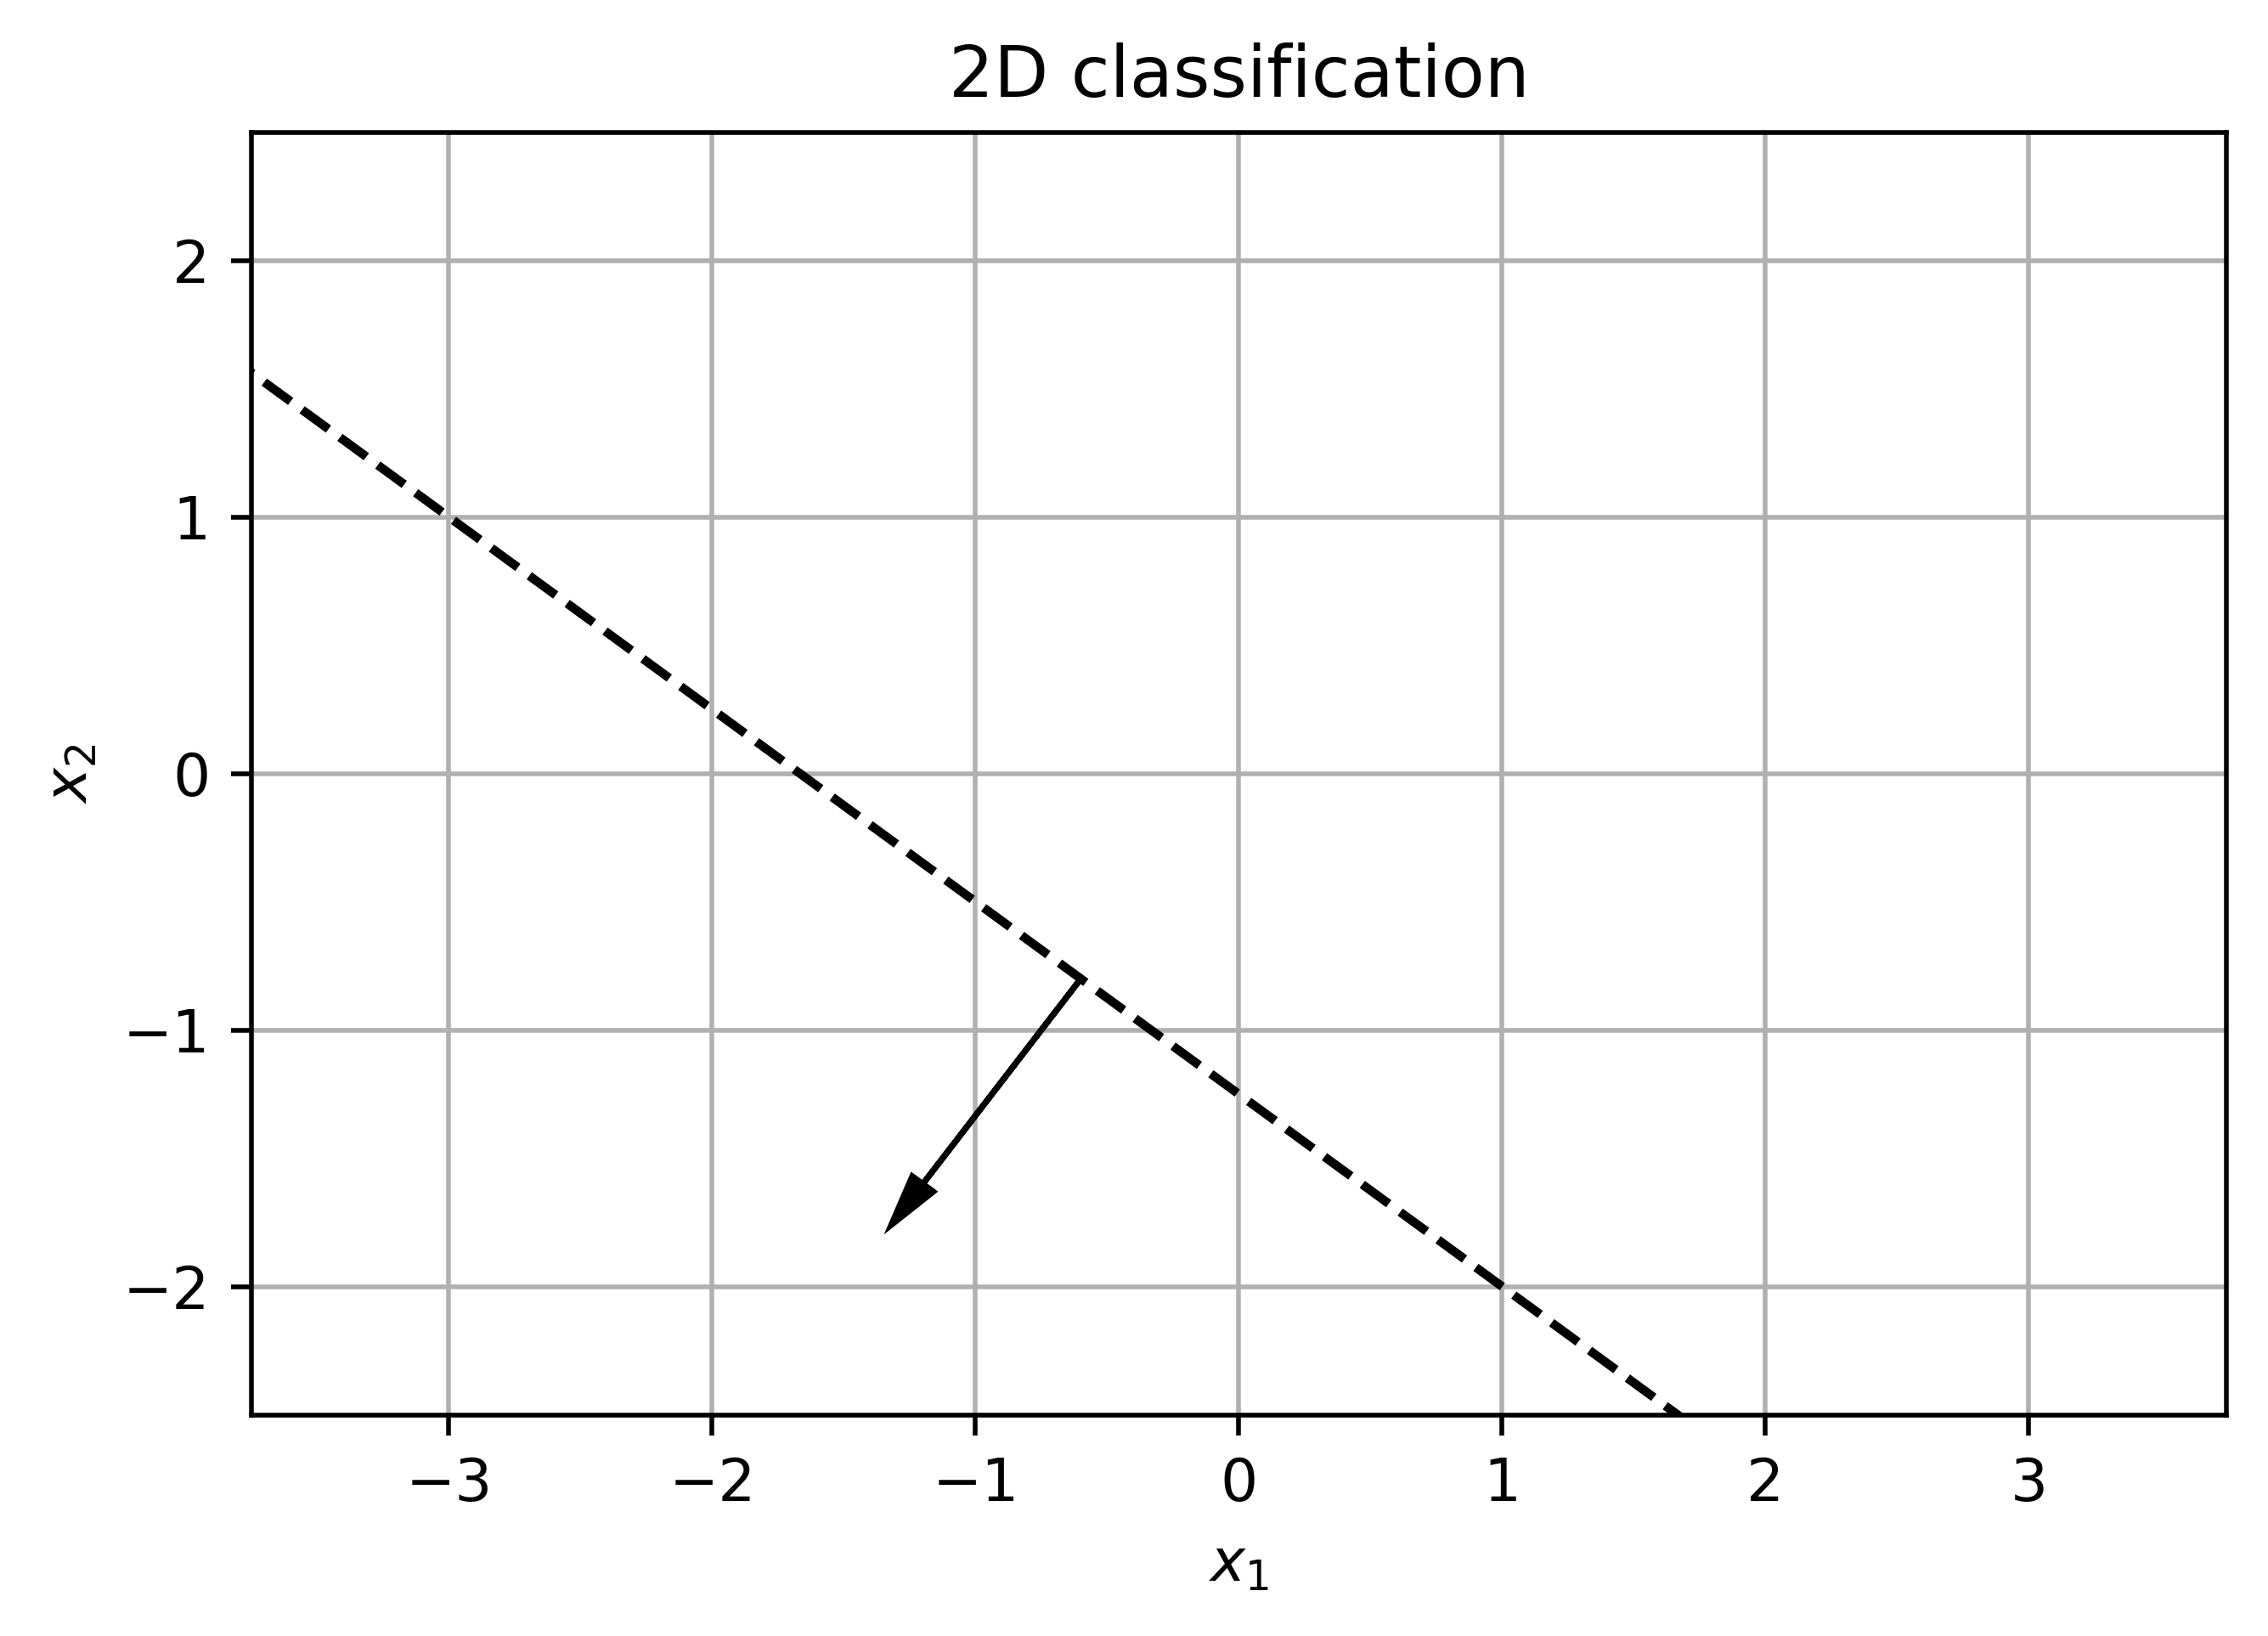
\includegraphics[width=70mm,scale=0.5]{images/classification_images/2d_classification_versus.png}

            \caption*{These two plots look almost the same, but represent completely different things!}
        \end{figure}
        
        Notice that these two plots are \textbf{both} plotted in 2-D, and both have a \textbf{line} plotted. But, they \textbf{aren't} as \textbf{similar} as they look. 
        
        Notice, for example, that the regression plot has \textbf{only} $x_1$, while the classification plot has $x_1$ \textbf{and} $x_2$.
        
        The reason why? The \textbf{output}.
        
        \begin{itemize}
            \item In \vocab{regression}, the output is a \textbf{real number}: every point on that line represents an input $x_1$, and an output $h(x_1)$.
                
                \begin{itemize}
                    \item This plot can only contain \textbf{one} input variable: the \textbf{second} axis is reserved for the \textbf{output}!
                \end{itemize}
            
            \item In \vocab{classification}, the output is \textbf{binary}. So, that line represents only the \textbf{values} where the output is $h(x)=0$. 
                \begin{itemize}
                    \item This plot can contain \textbf{two} input variables: $x_1$ and $x_2$. Rather than \textbf{displaying} the output, we only show one \textbf{slice} of the output: the $h(x)=0$ slice.
                \end{itemize}
        \end{itemize}
        
        If we think in terms of $f(x) = \theta^Tx +\theta_0$, we can compare them directly.
        
        The regression plot shows the exact value on the y-axis. If we want to know what $f(x_1=1)$ looks like, we can check the plot: we just get $f(1)=-2$.
        
        \begin{figure}[H]
            \centering
            
            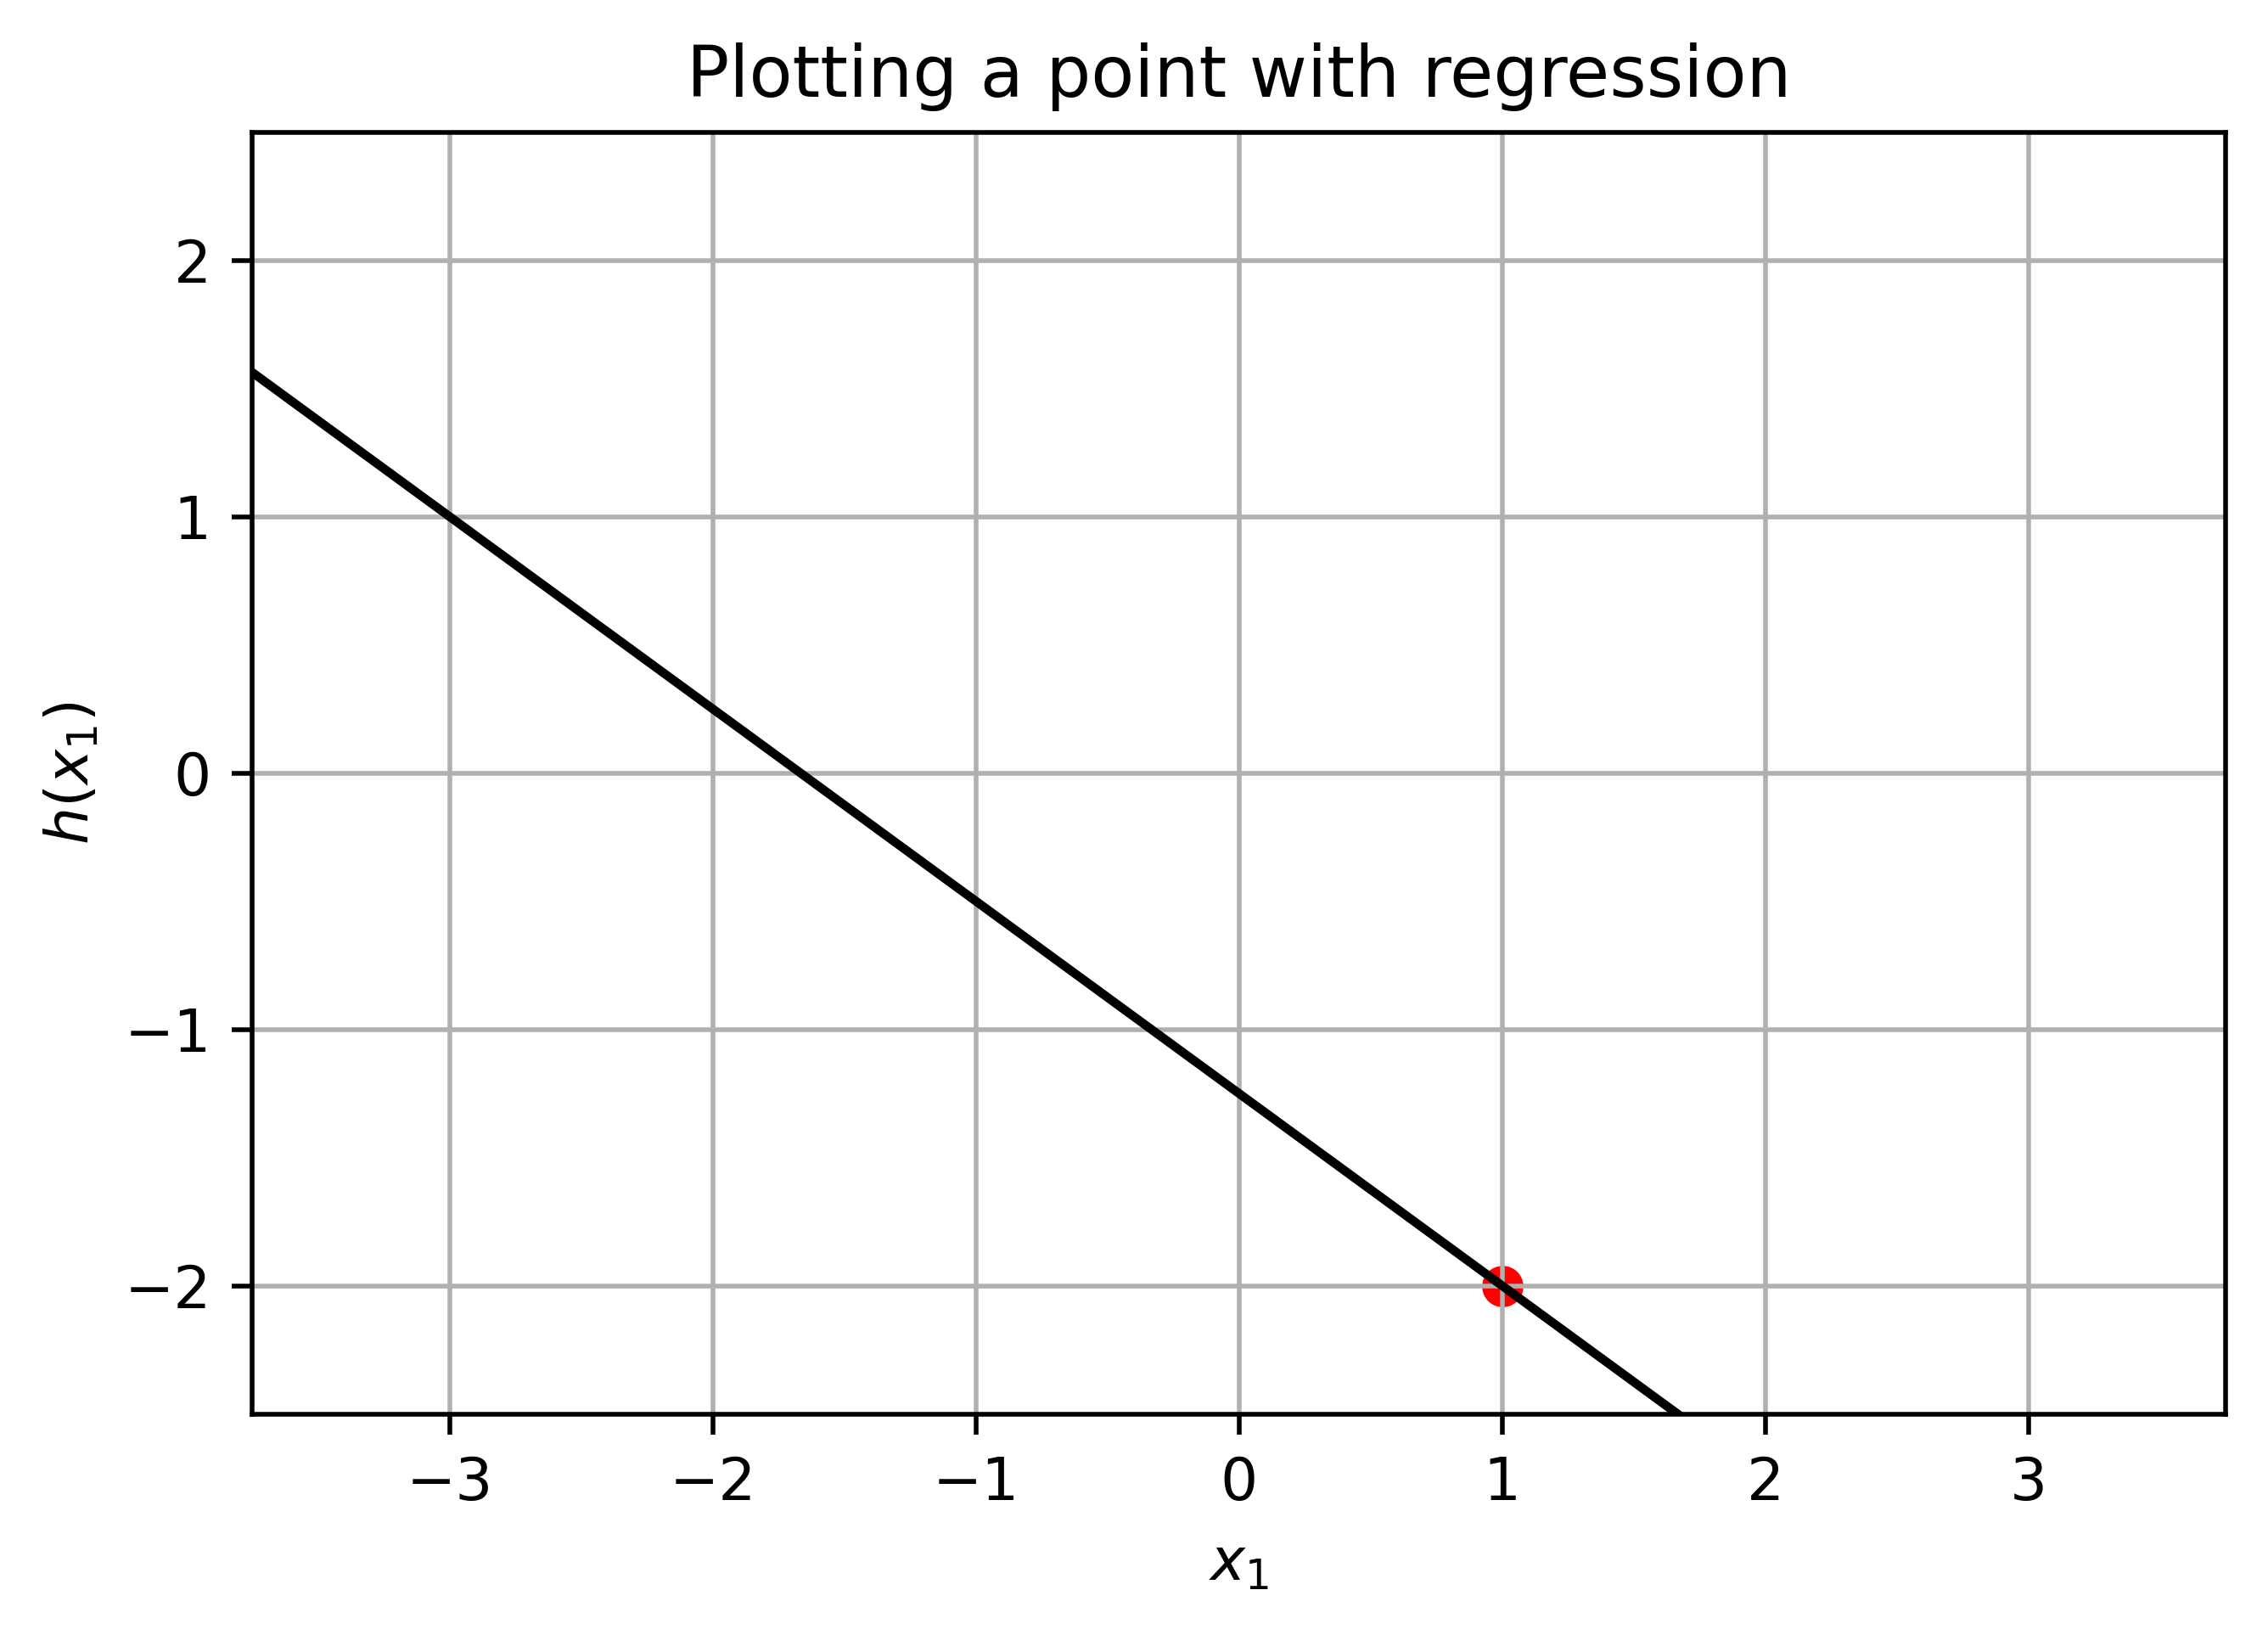
\includegraphics[width=70mm,scale=0.5]{images/classification_images/2d_regression_plot.png}
            \caption*{We have one input, and we get the exact value of our output.}
        \end{figure}
        
        But the classification plot \textbf{doesn't}! We aren't given the value of $\theta^Tx +\theta_0$ at $x=(1,0)$: we just know that it's \textbf{negative}.
        
        \begin{figure}[H]
            \centering
            
            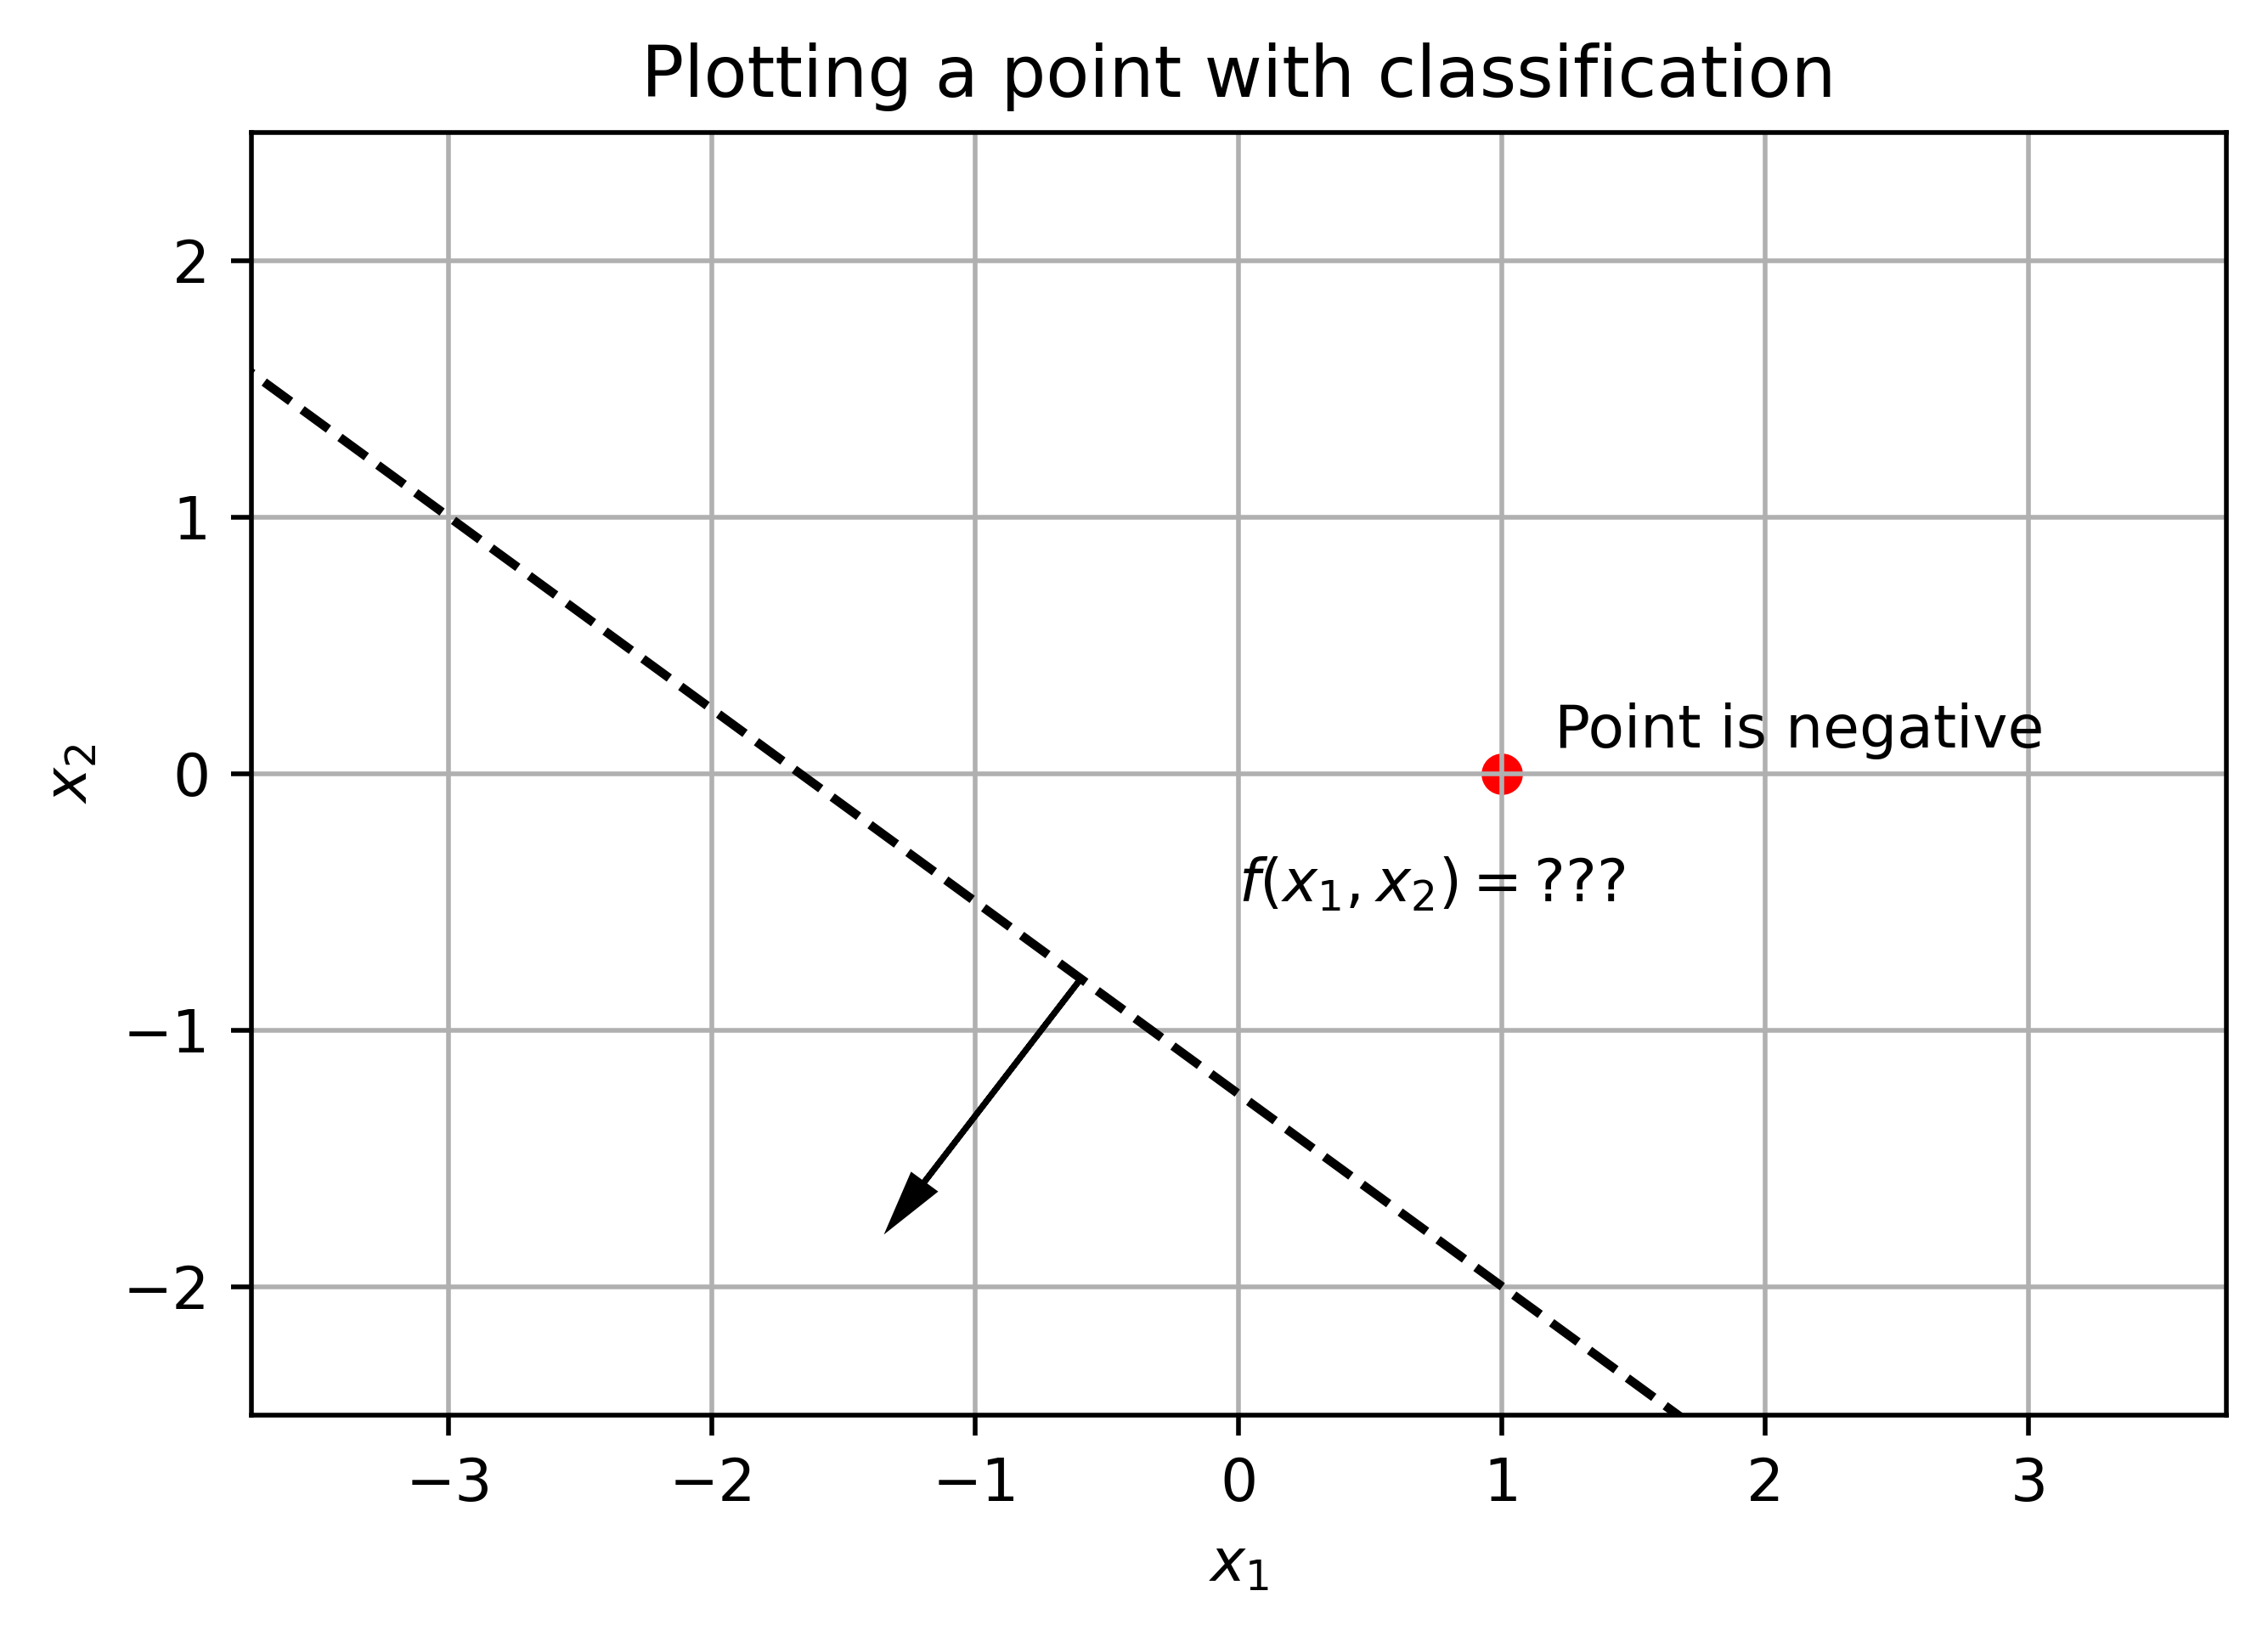
\includegraphics[width=70mm,scale=0.5]{images/classification_images/2d_classification_plot.png}
            \caption*{We have two input, and we \textbf{don't} get the exact output.}
        \end{figure}
        
        If we wanted to know the exact value of our 2-D classification, we would need to view it as a plane in 3-D space.
        
        This is the trade-off between these two plots: one gives more information about the output, and the other allows for more inputs in a lower dimension.\\
        
        \begin{clarification}
            \vocab{Regression} and \vocab{classification} plots that look the same, have \vocab{different functions}: 
            
            When looking at the output of $f(x)=\theta^T x + \theta_0$,
            \begin{itemize}
                \item A \purp{regression} plot gives the \gren{exact numeric} $f(x)$.
                
                \item A \purp{classification} plot only gives the \gren{sign} of the $f(x)$.
            \end{itemize}
            
            When plotting $n$ inputs,
                \begin{itemize}
                    \item A \purp{regression} plot uses a $d+1$ dimensions ($d$-dim hyperplane) to plot: +1 for the \gren{output}.
                    \item A \purp{classification} plot only needs $d$ dimensions ($(d-1)$-dim hyperplane): we only see the $f(x)=0$ \gren{hyperplane}.
                \end{itemize}
        \end{clarification}
        
        Why do we need $d+1$ dimensions to plot a $d$-dimensional \textbf{hyperplane}? You can think of it this way: a \textbf{line} in 2-D space is a 1-D \textbf{hyperplane}: we have only \textbf{one axis} we can move on the line.
            
        \begin{figure}[H]
            \centering
            
            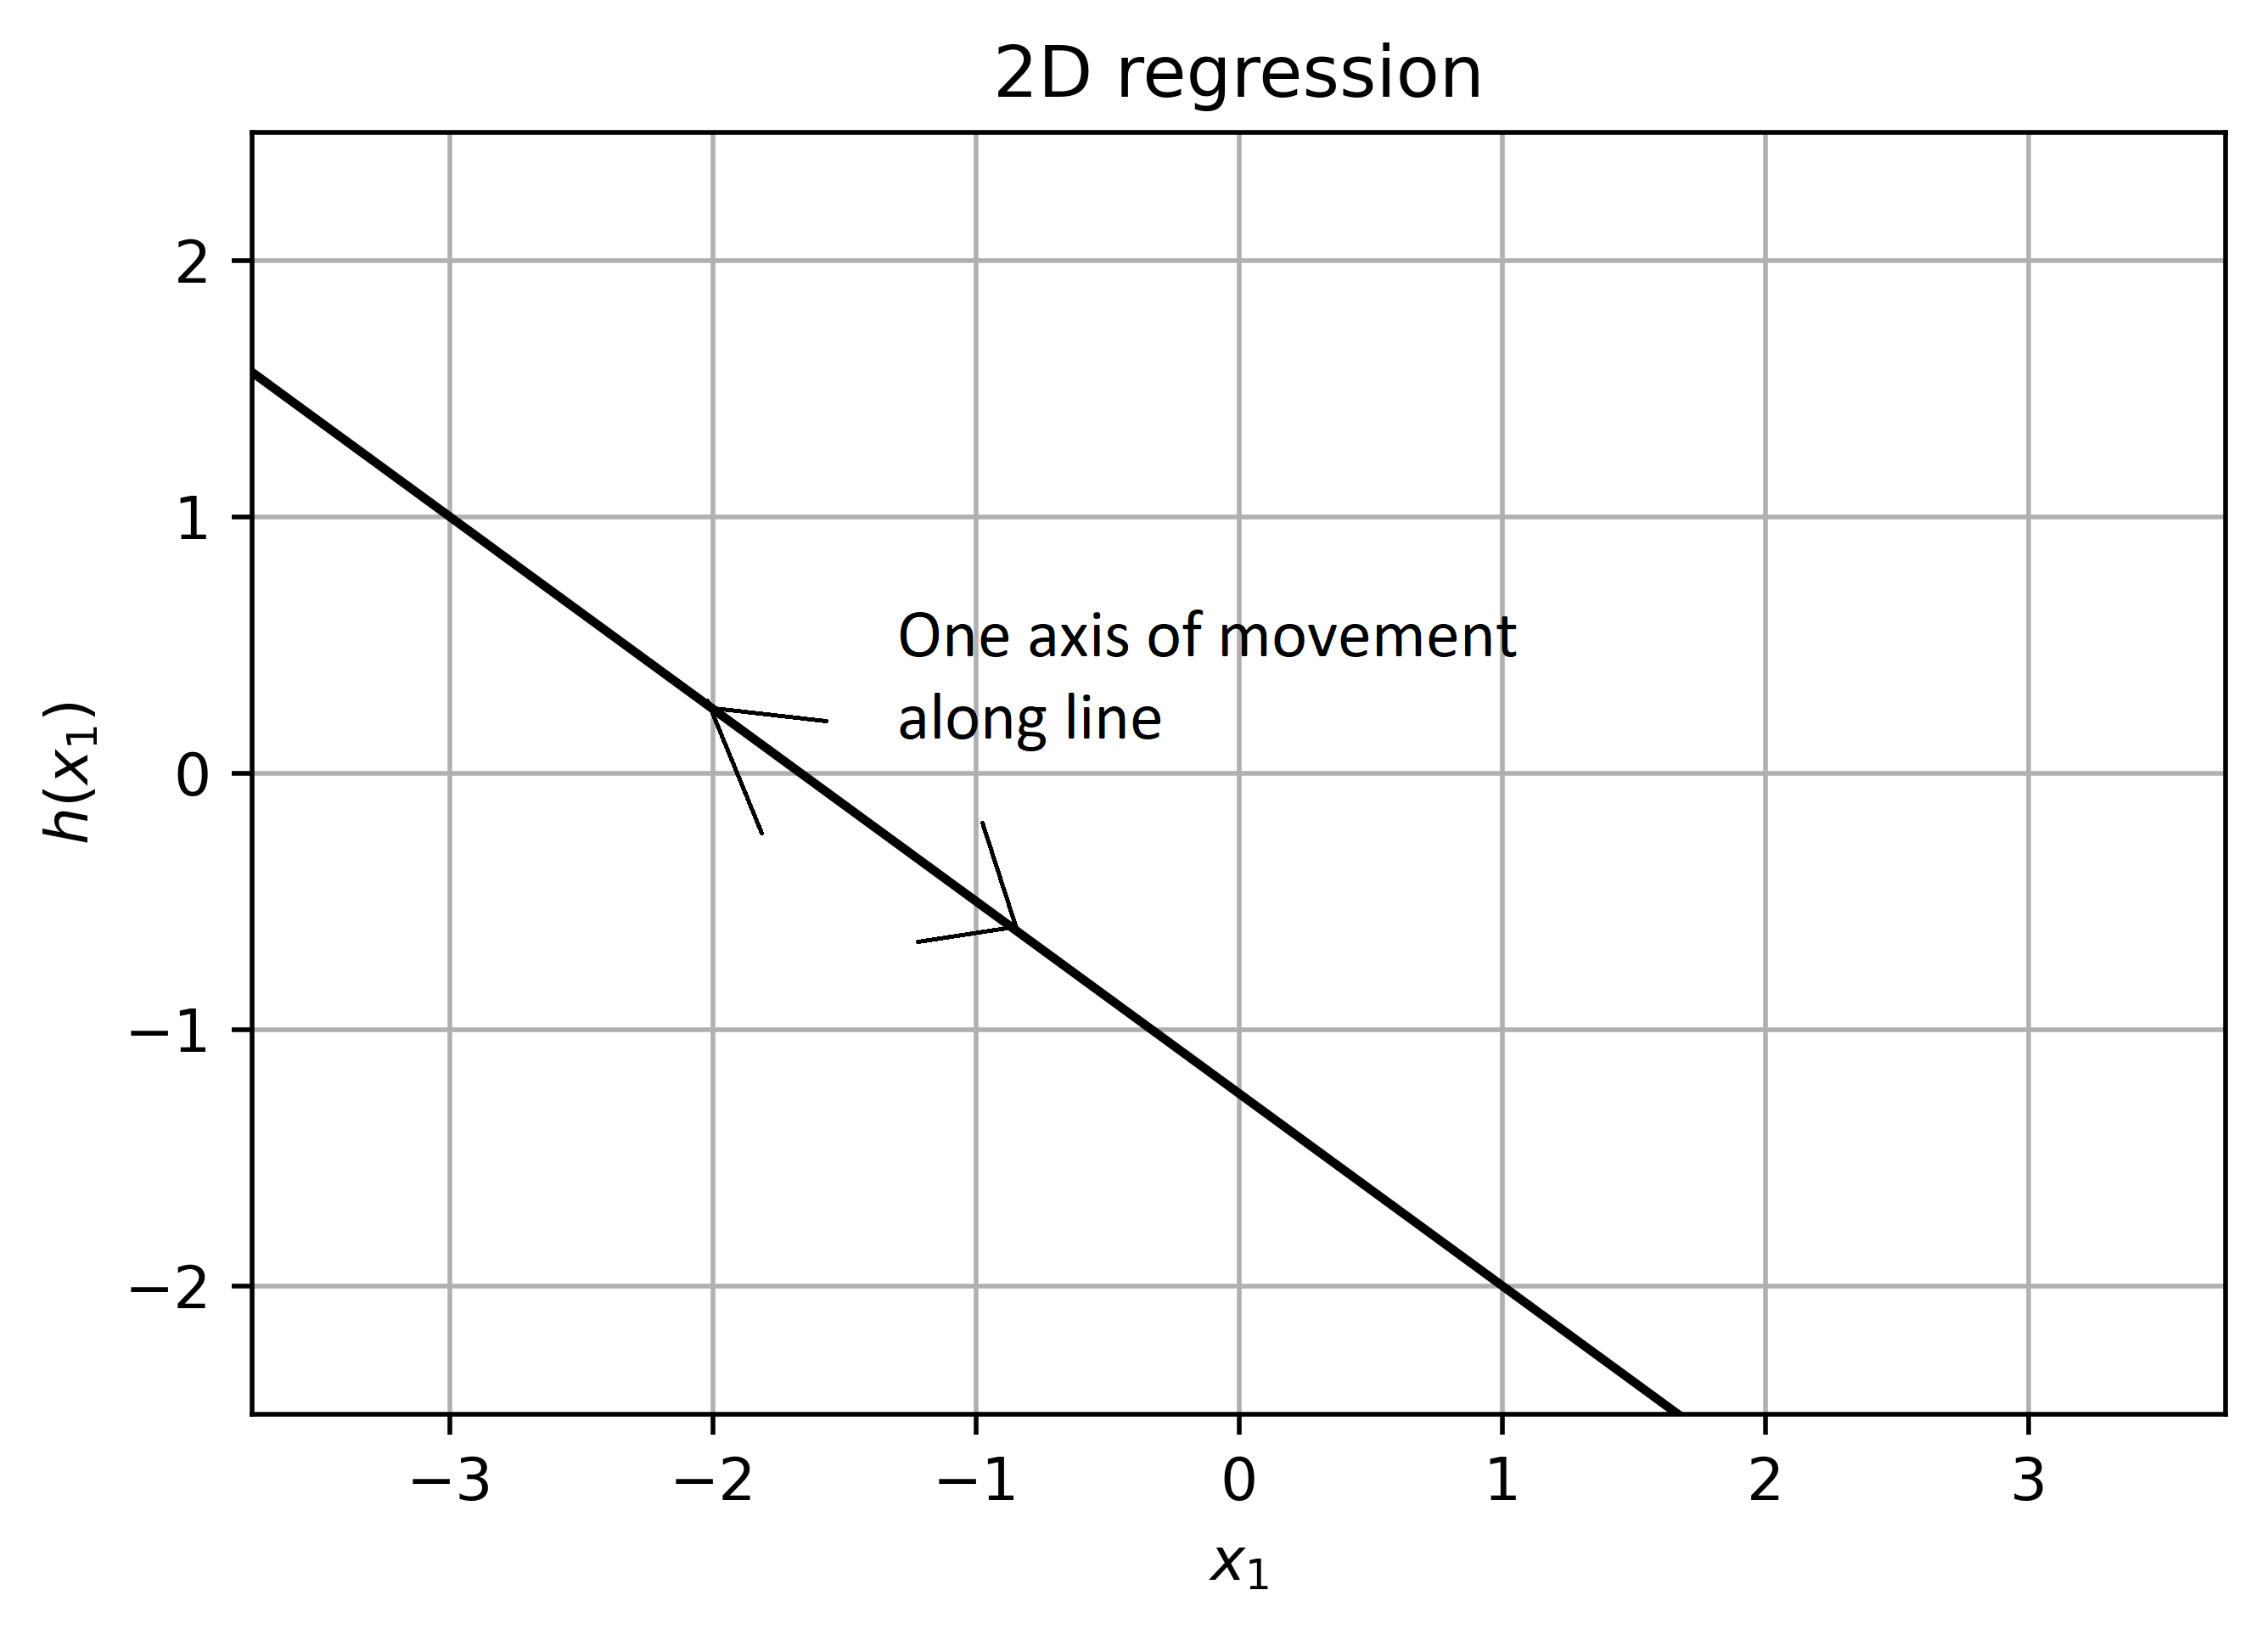
\includegraphics[width=70mm,scale=0.5]{images/classification_images/2d_regression_1d_hyperplane.png}
            \caption*{Our plot is 2-D, but we can only move along one axis on our line!}
        \end{figure}    
        
        Because of these differences, $\theta$ also acts differently:\\
        
        \begin{clarification}
            $\theta$ appears differently in 2-D regression and classification:
            
            \begin{itemize}
                \item In \vocab{2-D regression}, $\theta$ is the \purp{slope} of the line
                
                    \begin{equation}
                        h(x) = \theta x + \theta_0
                    \end{equation}
                
                \item In \vocab{2-D classification}, $\theta$ is the \purp{normal vector} of the line
                
                    \begin{equation}
                        0 = \theta^T x + \theta_0
                    \end{equation}
                
            \end{itemize}
        \end{clarification}
        
    \subsection{3d plot of 2d separator}
    
        For additional understanding, you might view the full output of $\theta^T x + \theta_0$, before we simplify the output to $\{-1,+1\}$.
        
        \begin{figure}[H]
            \centering
            
            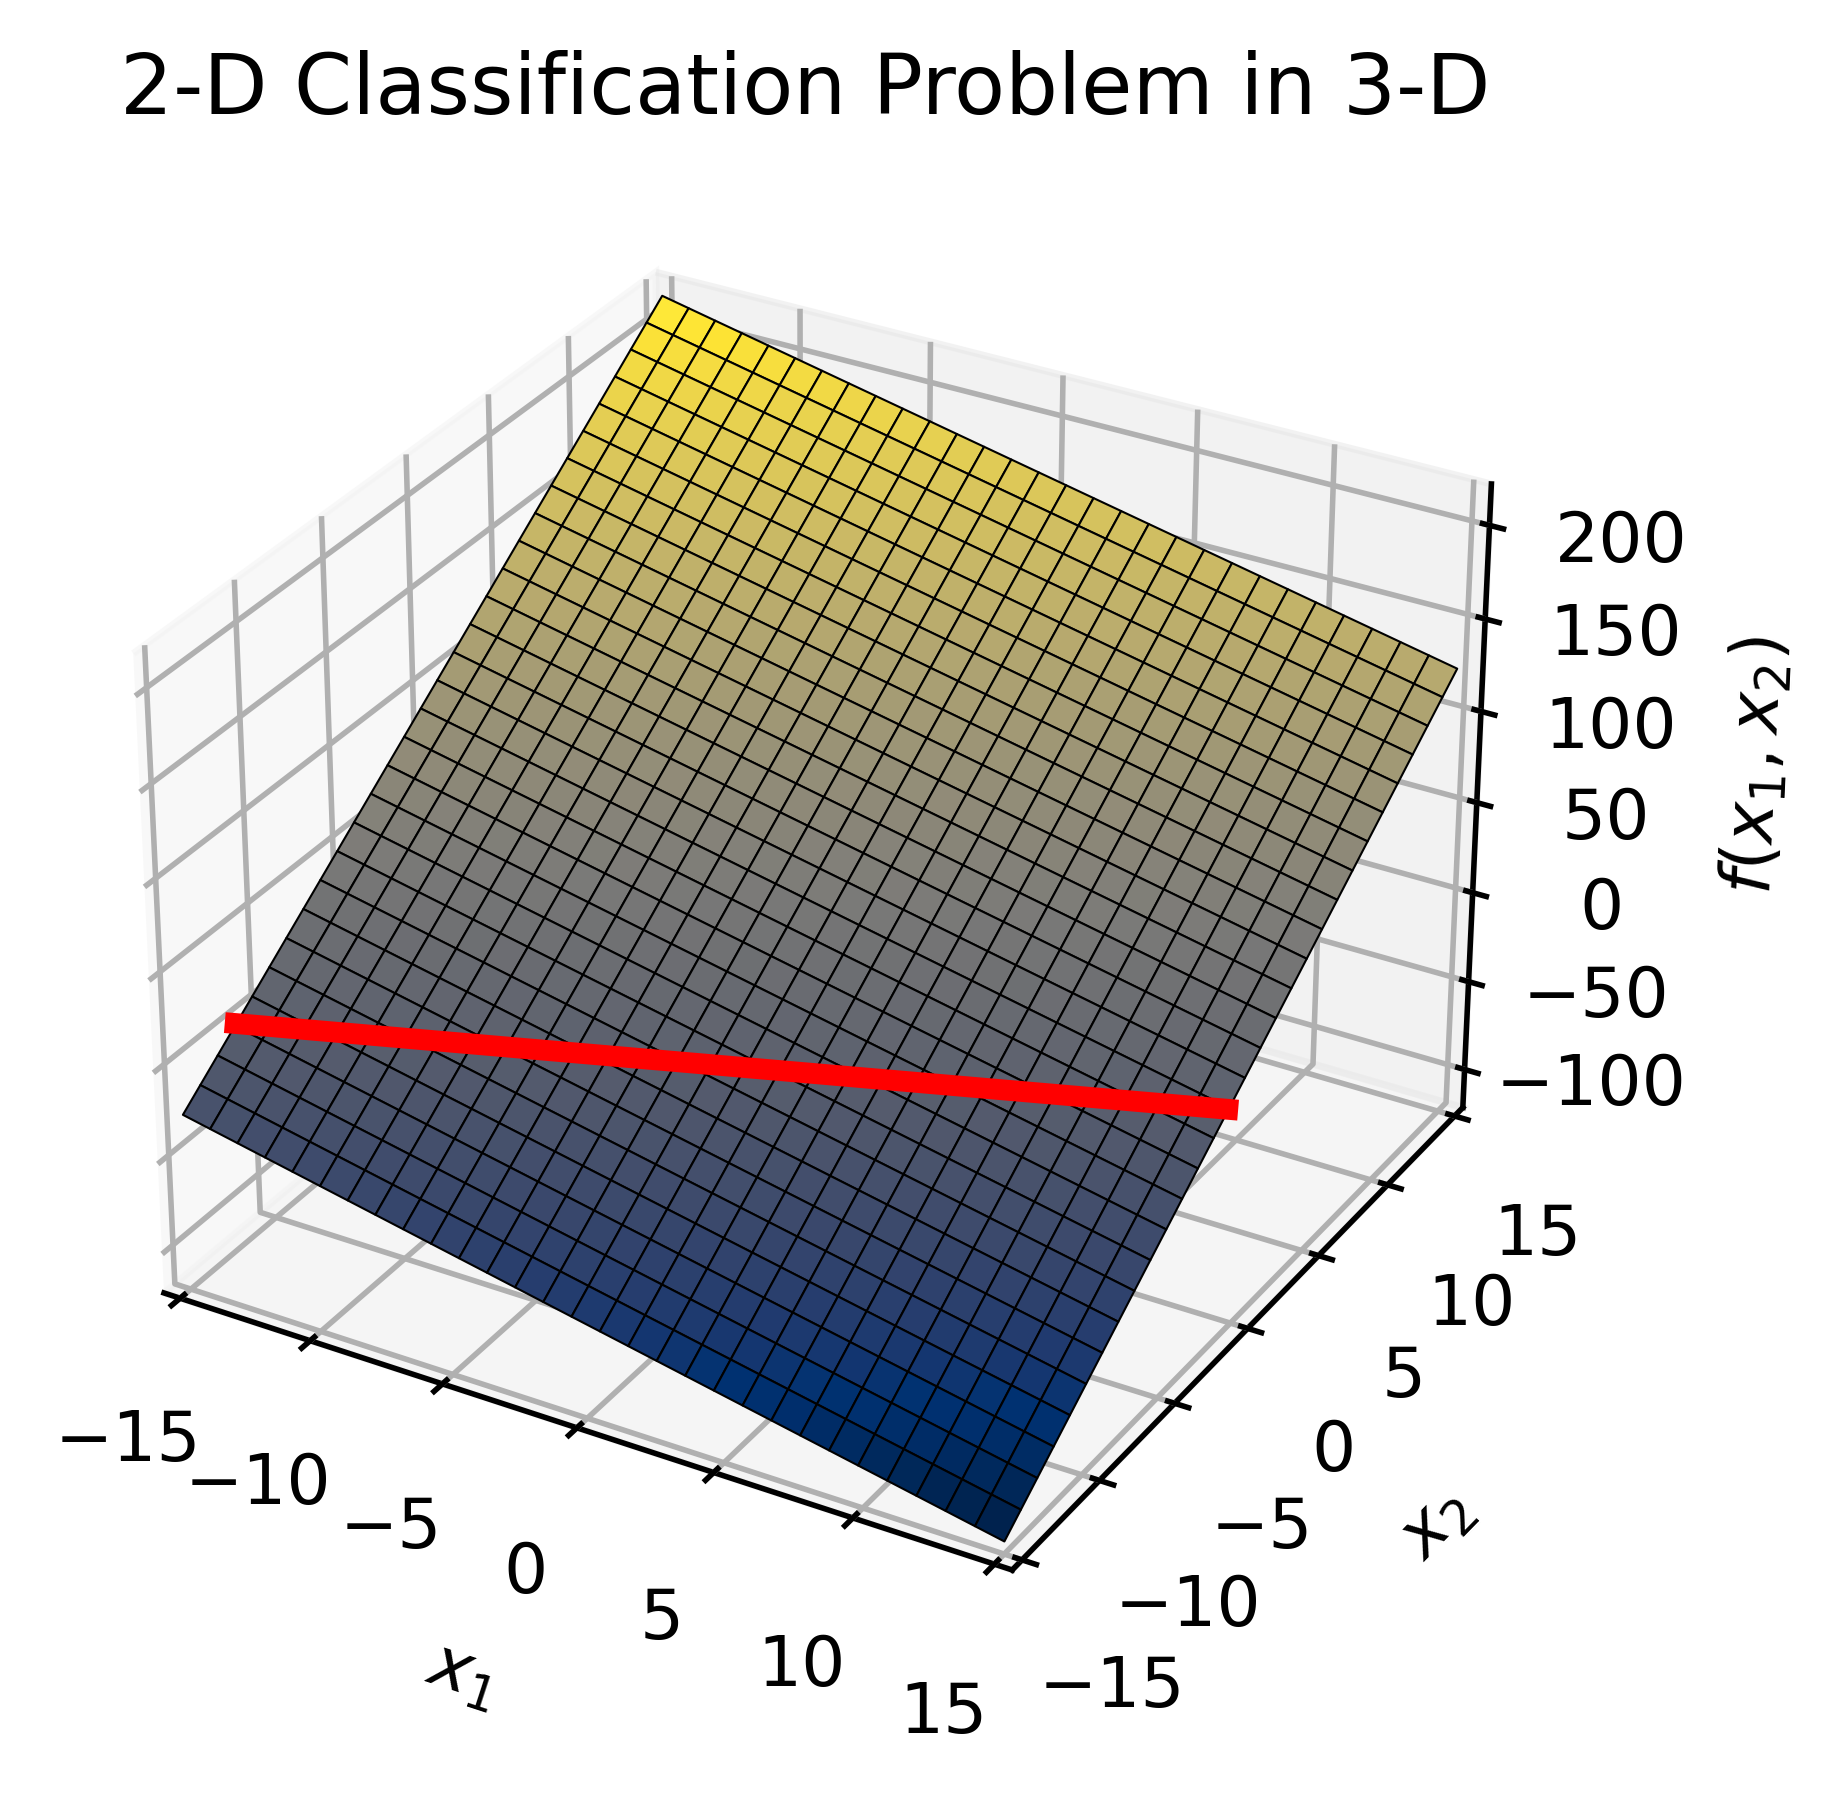
\includegraphics[width=70mm,scale=0.5]{images/classification_images/2d_classification_in_3d.png}
            \caption*{The red line represents where $f(x)=0$. The black line is our \textbf{normal vector}: notice that it's normal to the \textbf{line}, not the \textbf{plane}.}
        \end{figure}
        
        We mentioned before that, if we wanted to show the exact value of $f(x)$ for our 2-D classifier, we'd need a 3-D plot (just like for regression).
        
        So here, we've done \textbf{exactly} that: the \textbf{height} is the output of $h(x)$.
        
        But, because we don't \textbf{care} about the \textbf{exact} output in classification, we usually only graph the \textbf{red line}: where $f(x)=0$.
        
        This shows how we're taking a 2D slice ($f(x)=0$) out of a 3-D plot (full hyperplane), to \textbf{save} on one dimension of \textbf{plotting}.
    
    \subsection{Separable vs Non-separable data}
    
        One more consideration: \textbf{not all} data can be correctly \textbf{divided} by a linear separator!
        
        \begin{figure}[H]
            \centering
            
            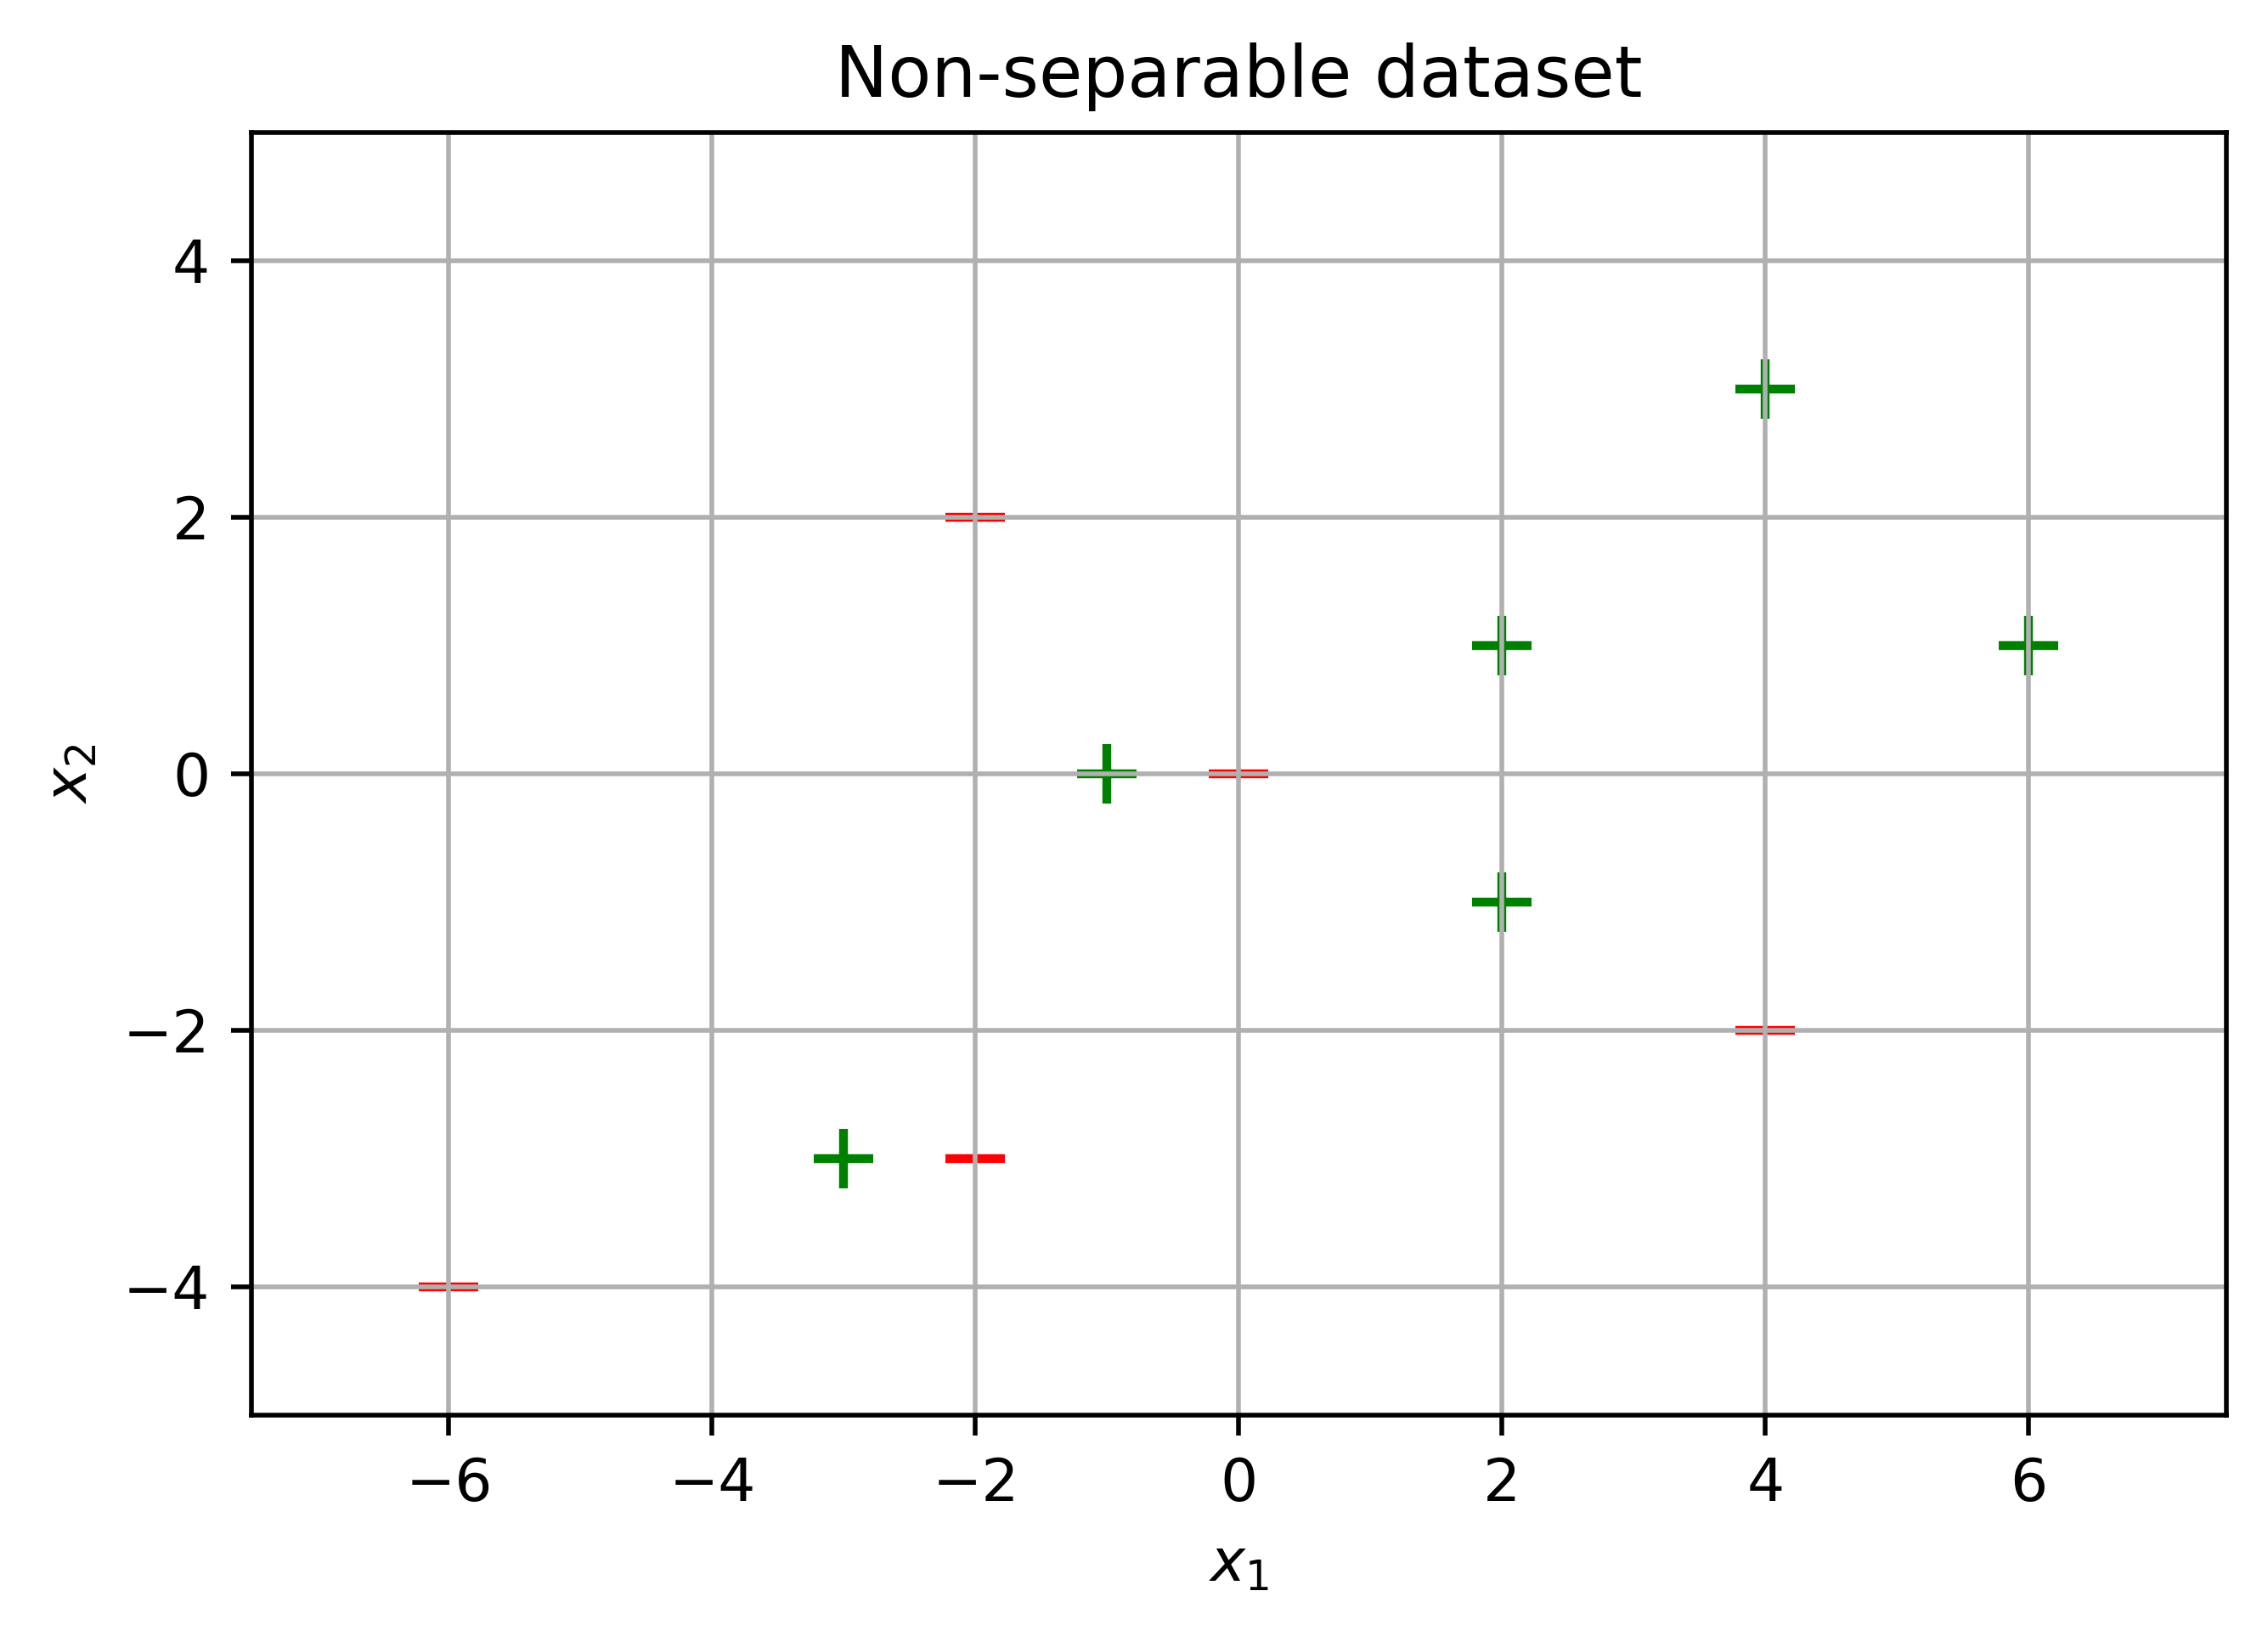
\includegraphics[width=70mm,scale=0.5]{images/classification_images/non_separable_dataset.png}
            \caption*{There's no line we could draw through this data to \textbf{separate} the points from each other.}
        \end{figure}
            
        If we can, we call it \textbf{linearly separable}.\\
        
        \begin{definition}
            A \gren{dataset} is \vocab{linearly separable} if you can \purp{perfectly} classify it with a \gren{linear classifier}.
        \end{definition}
        
        A couple common reasons for data to not be linearly separable:
        
        \begin{itemize}
            \item A positive and negative data point have the exact\textbf{ same position} in input space.
            
            \item Two points on either \textbf{side} of a point with opposite classification: $+-+$ or $-+-$, for example.
        \end{itemize}
        
        Very often, real-world datasets \textbf{can't} linearly separated, because of \textbf{complexities} in the real world, or random \textbf{noise}.
        
        But, sometimes, we can \textbf{almost} linearly separate it: we get very high \textbf{accuracy}. In those cases, it may be \textbf{fine} to use a linear separator: we might risk \textbf{overfitting} if we use a more complex model.
            \note{What is "high enough accuracy"? Depends on what you need it for!}
        
        Still, if a dataset is not \textbf{linearly separable}, or at least \textbf{high-accuracy} with a linear separator, that could mean we need a \textbf{richer} hypothesis class. 
            \note{Remember: a "richer" or more "expressive" hypothesis class is one that can create more hypotheses that our current one can't!}
        
        We'll get into ways to make a \textbf{richer} class in the \textbf{next} chapter: \textbf{feature transformations}.

\pagebreak
%%%%%%%%%%%%%%%%%%%%%%%%%%%%%%%%%%%%%%%%%%%%%%%%%%%%%%%%%%%%%%%%%%%%%%%%%%%%%

\section{Linear Logistic Classifiers}

    \subsection{The problem}

        Now, our goal is to create a \textbf{good model} for our problem, \textbf{binary classification}.
        
        To do this, we can \textbf{try} using our 0-1 loss $\loss$:
        
        \begin{equation}
            J(\theta, \theta_0) = 
            \frac{1}{n} \sum_{i=1}^n 
            \loss
            (
                \red{
                    \text{sign}(\theta^T\ex{x}{i} + \theta_0)
                    }, 
                \ex{y}{i}
            )
        \end{equation}
        
        The \textbf{first} thing to note is that there isn't an easy \textbf{analytical} solution, no simple \textbf{equation}: sign$(u)$ isn't a function that we can explicitly \textbf{solve}, like we could for \textbf{linear regression}.
            \note{To be fair, this is true for most possible problems: most of them can't be solved analytically.}
            
        So, we refer to our other approach, \textbf{gradient descent}.
        
        But in order to do that, we'll just need to get the \textbf{gradient}.
        
        \begin{equation}
            \nabla_\theta J = 0
        \end{equation}
        
        ...Well that's not good.
            \note{Why not? Because we use our \textbf{gradient} to decide \textbf{how} to change $\theta$, if the gradient is 0, we'll never \textbf{improve} $\theta$ at all!}
        
    \subsection{The real problem: sign$(u)$ is flat}
    
        What's going on here? Let's look at the sign function:
        
        \begin{figure}[H]
            \centering
            
            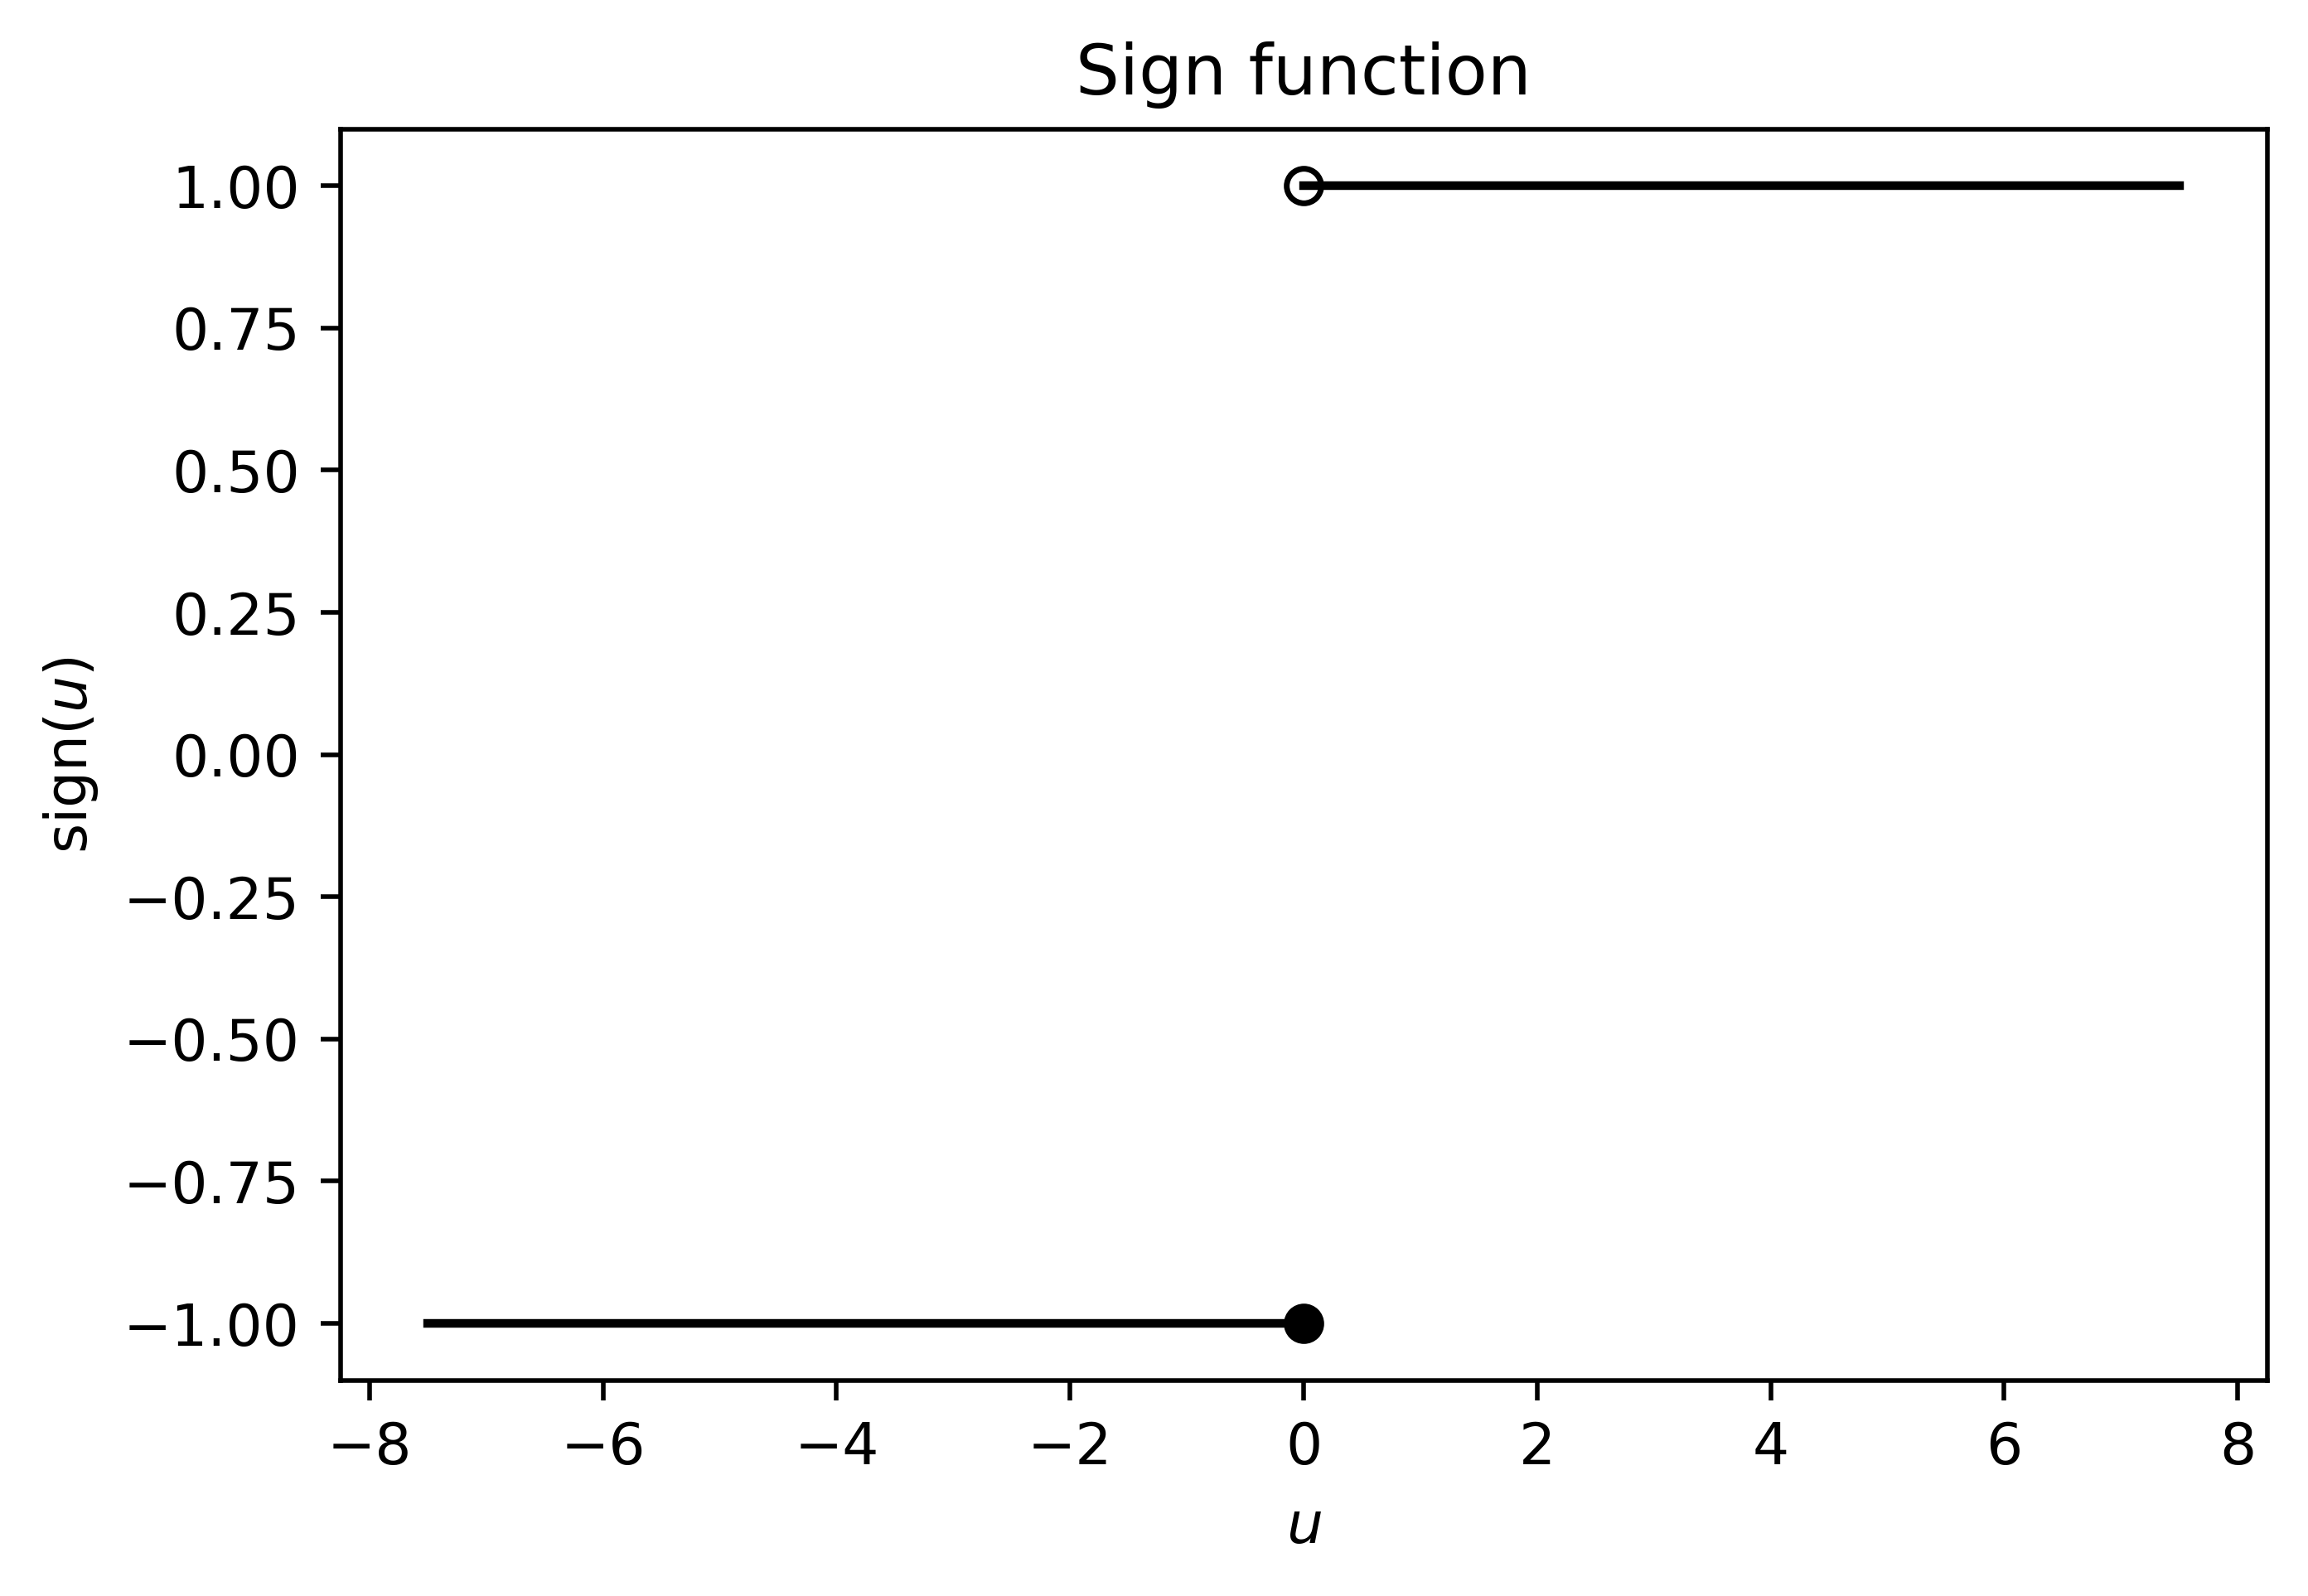
\includegraphics[width=70mm,scale=0.5]{images/classification_images/sign_function.png}
            \caption*{Sign is a flat function! The slope is 0 everywhere, except $u=0$, where it's \textbf{undefined}.}
        \end{figure}
        
        Well, that explains why we can't use the gradient: the function is \textbf{flat}.
        
        Another way to say this is that our function doesn't \textbf{tell} us when we're \textbf{closer} to being right.
        
        There's \textbf{no difference} between being \textbf{wrong} by 1 unit or being wrong by 10 units: you can't tell if you're getting \textbf{closer} to a correct answer.
        
        And the \textbf{gradient} doesn't tell you which way to move in \textbf{parameter space} to further improve.
            \note{Remember, parameter space is what we move through as we change our parameter vector $\theta$.}
        
        In fact, the best way we know how to approach this kind of problem takes \textbf{exponential} time: it takes exponentially \textbf{longer} to solve based on our \textbf{number} of data points.
        
        That's way too \textbf{slow}. So, we'll have to come up with a \textbf{better} function: something to \textbf{replace} sign$(u)$, that still serves the same role.\\
        
        \begin{concept}
            The \vocab{sign function} is difficult to optimize, because it isn't \purp{smooth}: not only is the slope undefined at 0, it is 0 everywhere else.
            
            This causes two problems:
            
            \begin{itemize}
                \item We can't tell whether one \gren{hypothesis} is \vocab{closer} to being \purp{correct}, if it has gotten \gren{better}, unless its accuracy has increased. 
                    \begin{itemize}
                        \item This makes it harder to \gren{improve}.
                    \end{itemize}
                
                \item We can't indicate how \purp{certain} we are in our answer: sign$(u)$ is \gren{all-or-nothing}: we choose one class, with no information about how \purp{confident} we are in our choice.
                    \begin{itemize}
                        \item Knowing how \purp{uncertain} we are can be \gren{helpful}, both for \gren{improving} our machine and also \gren{judging} the choices or machine makes.
                    \end{itemize}
            \end{itemize}
        \end{concept}
        
        So, we need to explore a \textbf{new} approach: we'll \textbf{replace} sign$(u)$ with something else.
    
    \subsection{The sigmoid function}
    
        So, what do we \textbf{replace} sign with? We like the way sign \textbf{works} (choosing between two different classes based on a \textbf{threshold}), so maybe we want a \textbf{smoother} version of it.
        
        \begin{figure}[H]
            \centering
            
            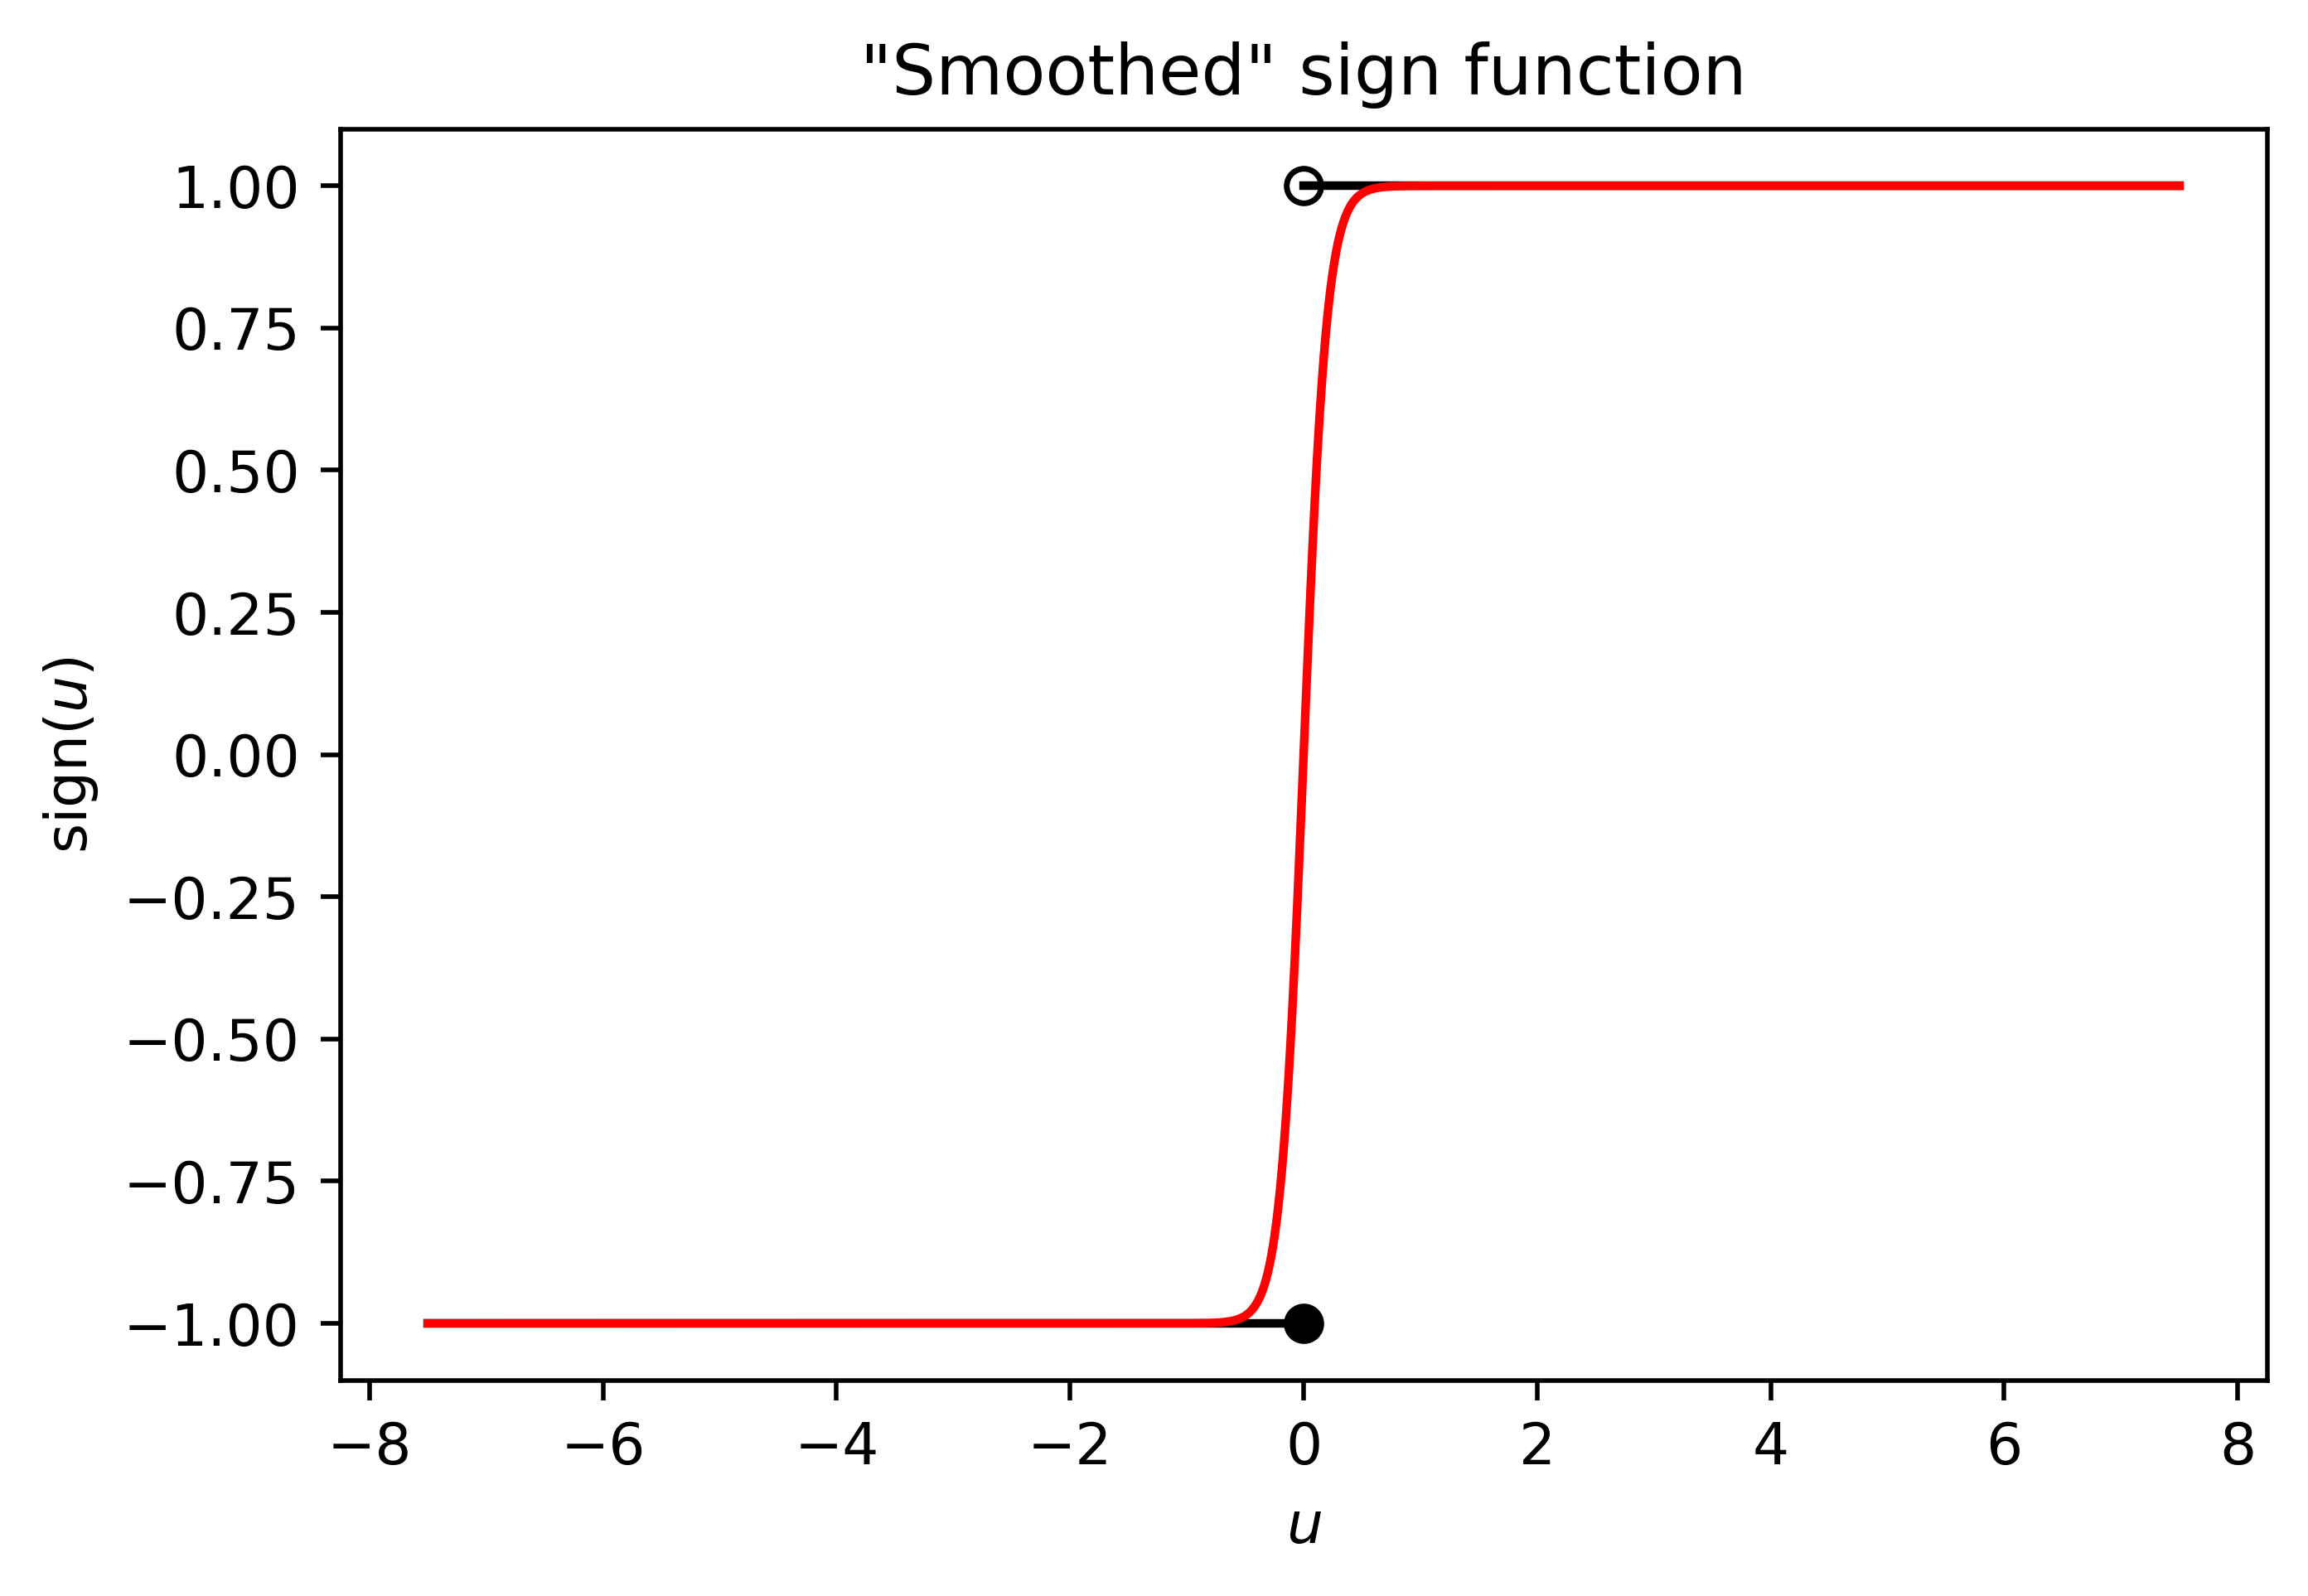
\includegraphics[width=70mm,scale=0.5]{images/classification_images/smoothed_sign_function.png}
            \caption*{The red line shows a "\textbf{smoother}" sign function, that mostly behaves the same, while solving our problem.}
        \end{figure}
        
        This solves \textbf{one} of our two problems: the \textbf{gradient} is \textbf{nonzero}. 
            \note{It's hard to see visually, but the function is \textbf{smooth}, and the slope is nonzero \textbf{everywhere}!}
        
        We could also make it less steep:
        
        \begin{figure}[H]
            \centering
            
            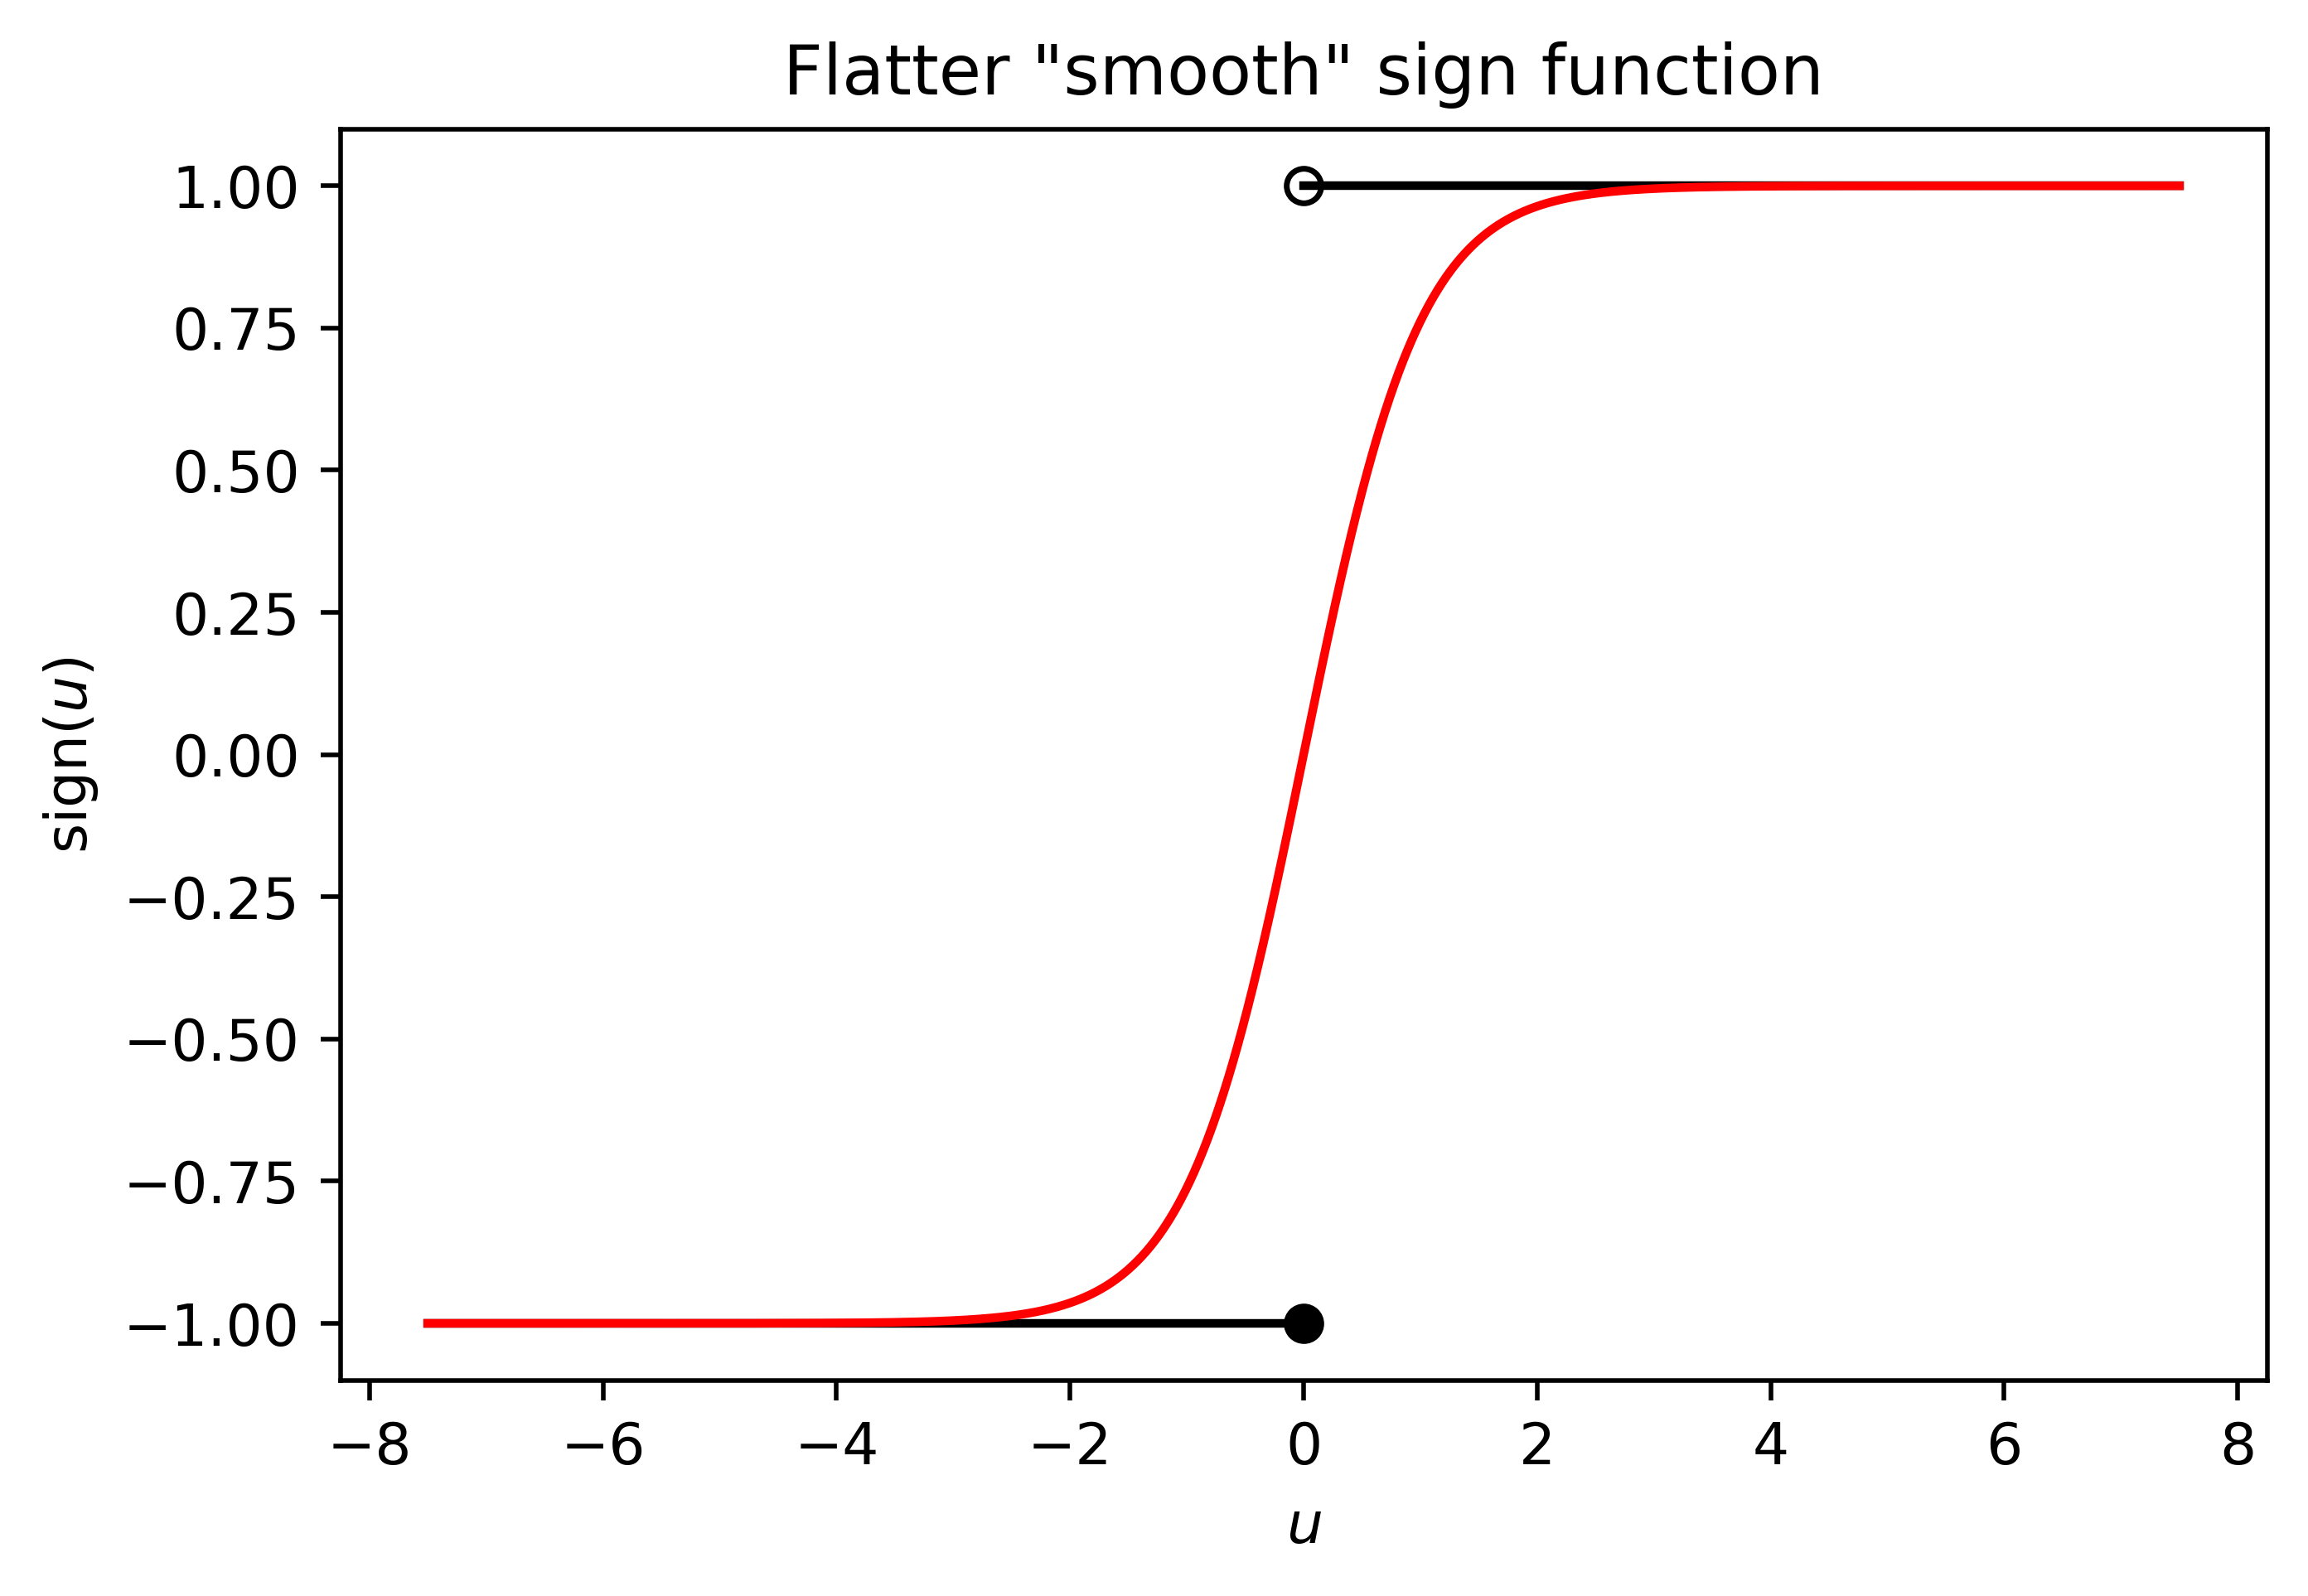
\includegraphics[width=70mm,scale=0.5]{images/classification_images/flatter_smooth_sign_function.png}
        \end{figure}
        
        So, we need a \textbf{function} that accomplishes this. It turns out there are \textbf{several} that work: $\tanh{u}$, for example.
        
        For our purposes, we'll use the following function:\\
        
        \begin{definition}
            The \vocab{sigmoid} function
            
            \begin{equation}
                \sigma(u) = \frac{1}{1+e^{-u}}
            \end{equation}
            
            ...is a \purple{nonlinear} function that we use to \gren{compute} the output of our \vocab{classification} problem.
            
            It is also called the \vocab{logistic} function.
        \end{definition}
        
        The function looks like this:
        
        \begin{figure}[H]
            \centering
            
            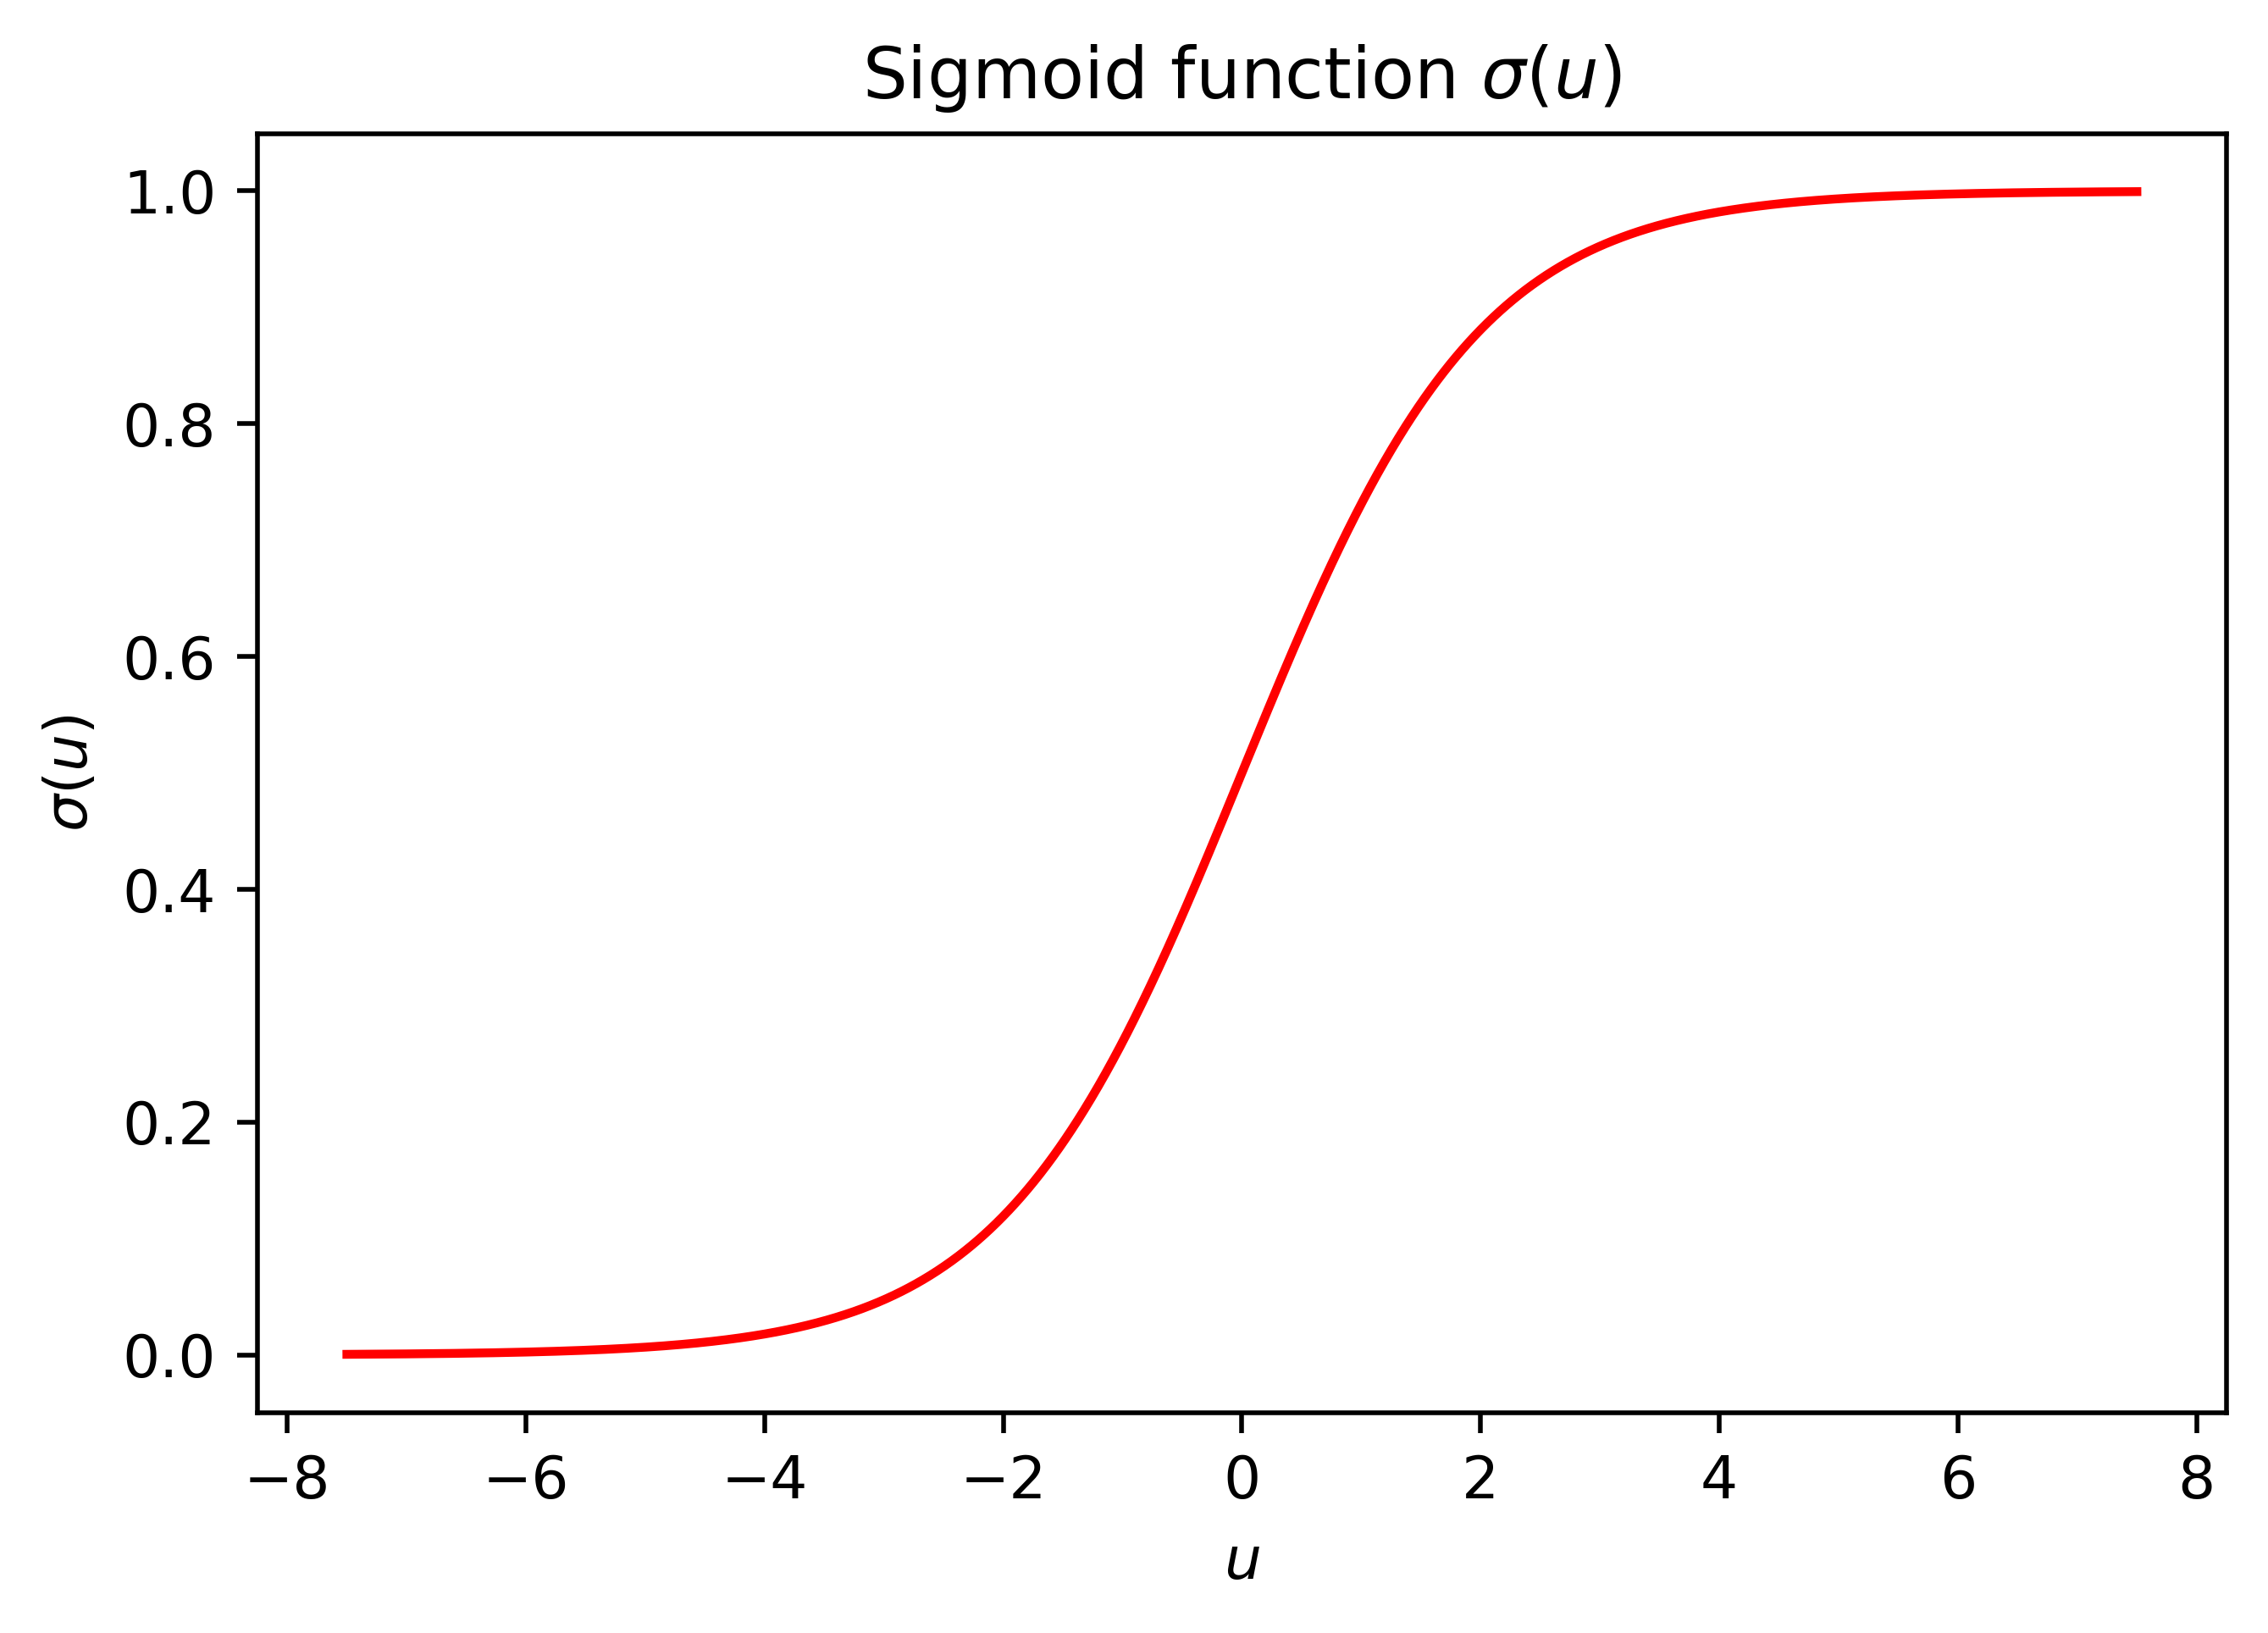
\includegraphics[width=70mm,scale=0.5]{images/classification_images/sigmoid_u.png}
        \end{figure}
        
    \subsection{Sigmoid as a probability}
        
        Something you may \textbf{notice} is that $\sigma(x)$ is always between 0 and 1. But before, sign$(x)$ was \textbf{always} between -1 and +1. Why would we use \textit{this} function?
        
        Because going between 0 and 1 has a different advantage: we can interpret it as a \textbf{probability}.
        
        Your \textbf{value} of $\sigma(u)$ can be stated as, "what does the machine think is the \textbf{probability} we \textbf{classify} this data point as +1".
        
        And, on the \textbf{flip} side, $1-\sigma(u)$ is the \textbf{probability} we \textbf{classify} as $-1$.
        
        This solves the second problem we mentioned \textbf{earlier}: we can indicate how \textbf{confident} the machine is in its answer!\\
        
        \begin{concept}
            The output of the \vocab{sigmoid function} $\sigma(\red{u(x)})$ gives the \purp{probability} that the data point $x$ is classified \gren{positively}.
            
            \begin{equation*}
                \quad \;\; \sigma(u) = \p{ x\text{ is classified }+1 }
            \end{equation*}
            \begin{equation*}
                1 - \sigma(u) = \p{ x\text{ is classified }-1 }
            \end{equation*}
            
            Note that this works because $\sigma(u) \in (0,1)$.
        \end{concept}
        
    \subsection{Logistic Regression}
    
        So, we've seen the benefits of switching from sign$(u)$ to $\sigma(u)$. So we'll do that:
            \note{We're using $u(x)=\theta^T x + \theta_0$}\\
        
        
        \begin{kequation}
            \vocab{Logistic Regression} is a \purp{modification} of \gren{linear regression}.
            
            \begin{equation*}
                h(x; \theta) = \sigma(\theta^T x + \theta_0 )
            \end{equation*}
        
            \centerline{where}
            
            \begin{equation*}
                \sigma(u) = \frac{1}{1+e^{-u}}
            \end{equation*}
            
            It outputs the \vocab{probability} of a \purp{positive} classification.
        \end{kequation}
        
        If we \textbf{plug} this in, we get this slightly ugly expression:
        
        \begin{equation*}
            h(x; \theta) = \frac{1}{1+e^{-(\theta^T x + \theta_0) } }
        \end{equation*}
        
        We have a problem, though: \textbf{logistic regression} is a... \vocab{regression} function. It takes in a real \textbf{vector}, and outputs a real \textbf{number}: $\RR^d \rightarrow \RR$.
        
        We can't use this to do \textbf{classification}, where want $\RR^d \rightarrow \{-1,+1\}$!
        
    \subsection{Prediction Threshold}
    
        When we were just using $u(x) = \theta^T x + \theta_0$, we classified data points by saying whether $u(x)>0$. Our boundary was $u(x)=0$.
        
        We can't quite do that here, because $\sigma(u)=0$ is \textbf{impossible}: $\sigma(u)$ is \textbf{always} greater than 0.
        
        \begin{figure}[H]
            \centering
            
            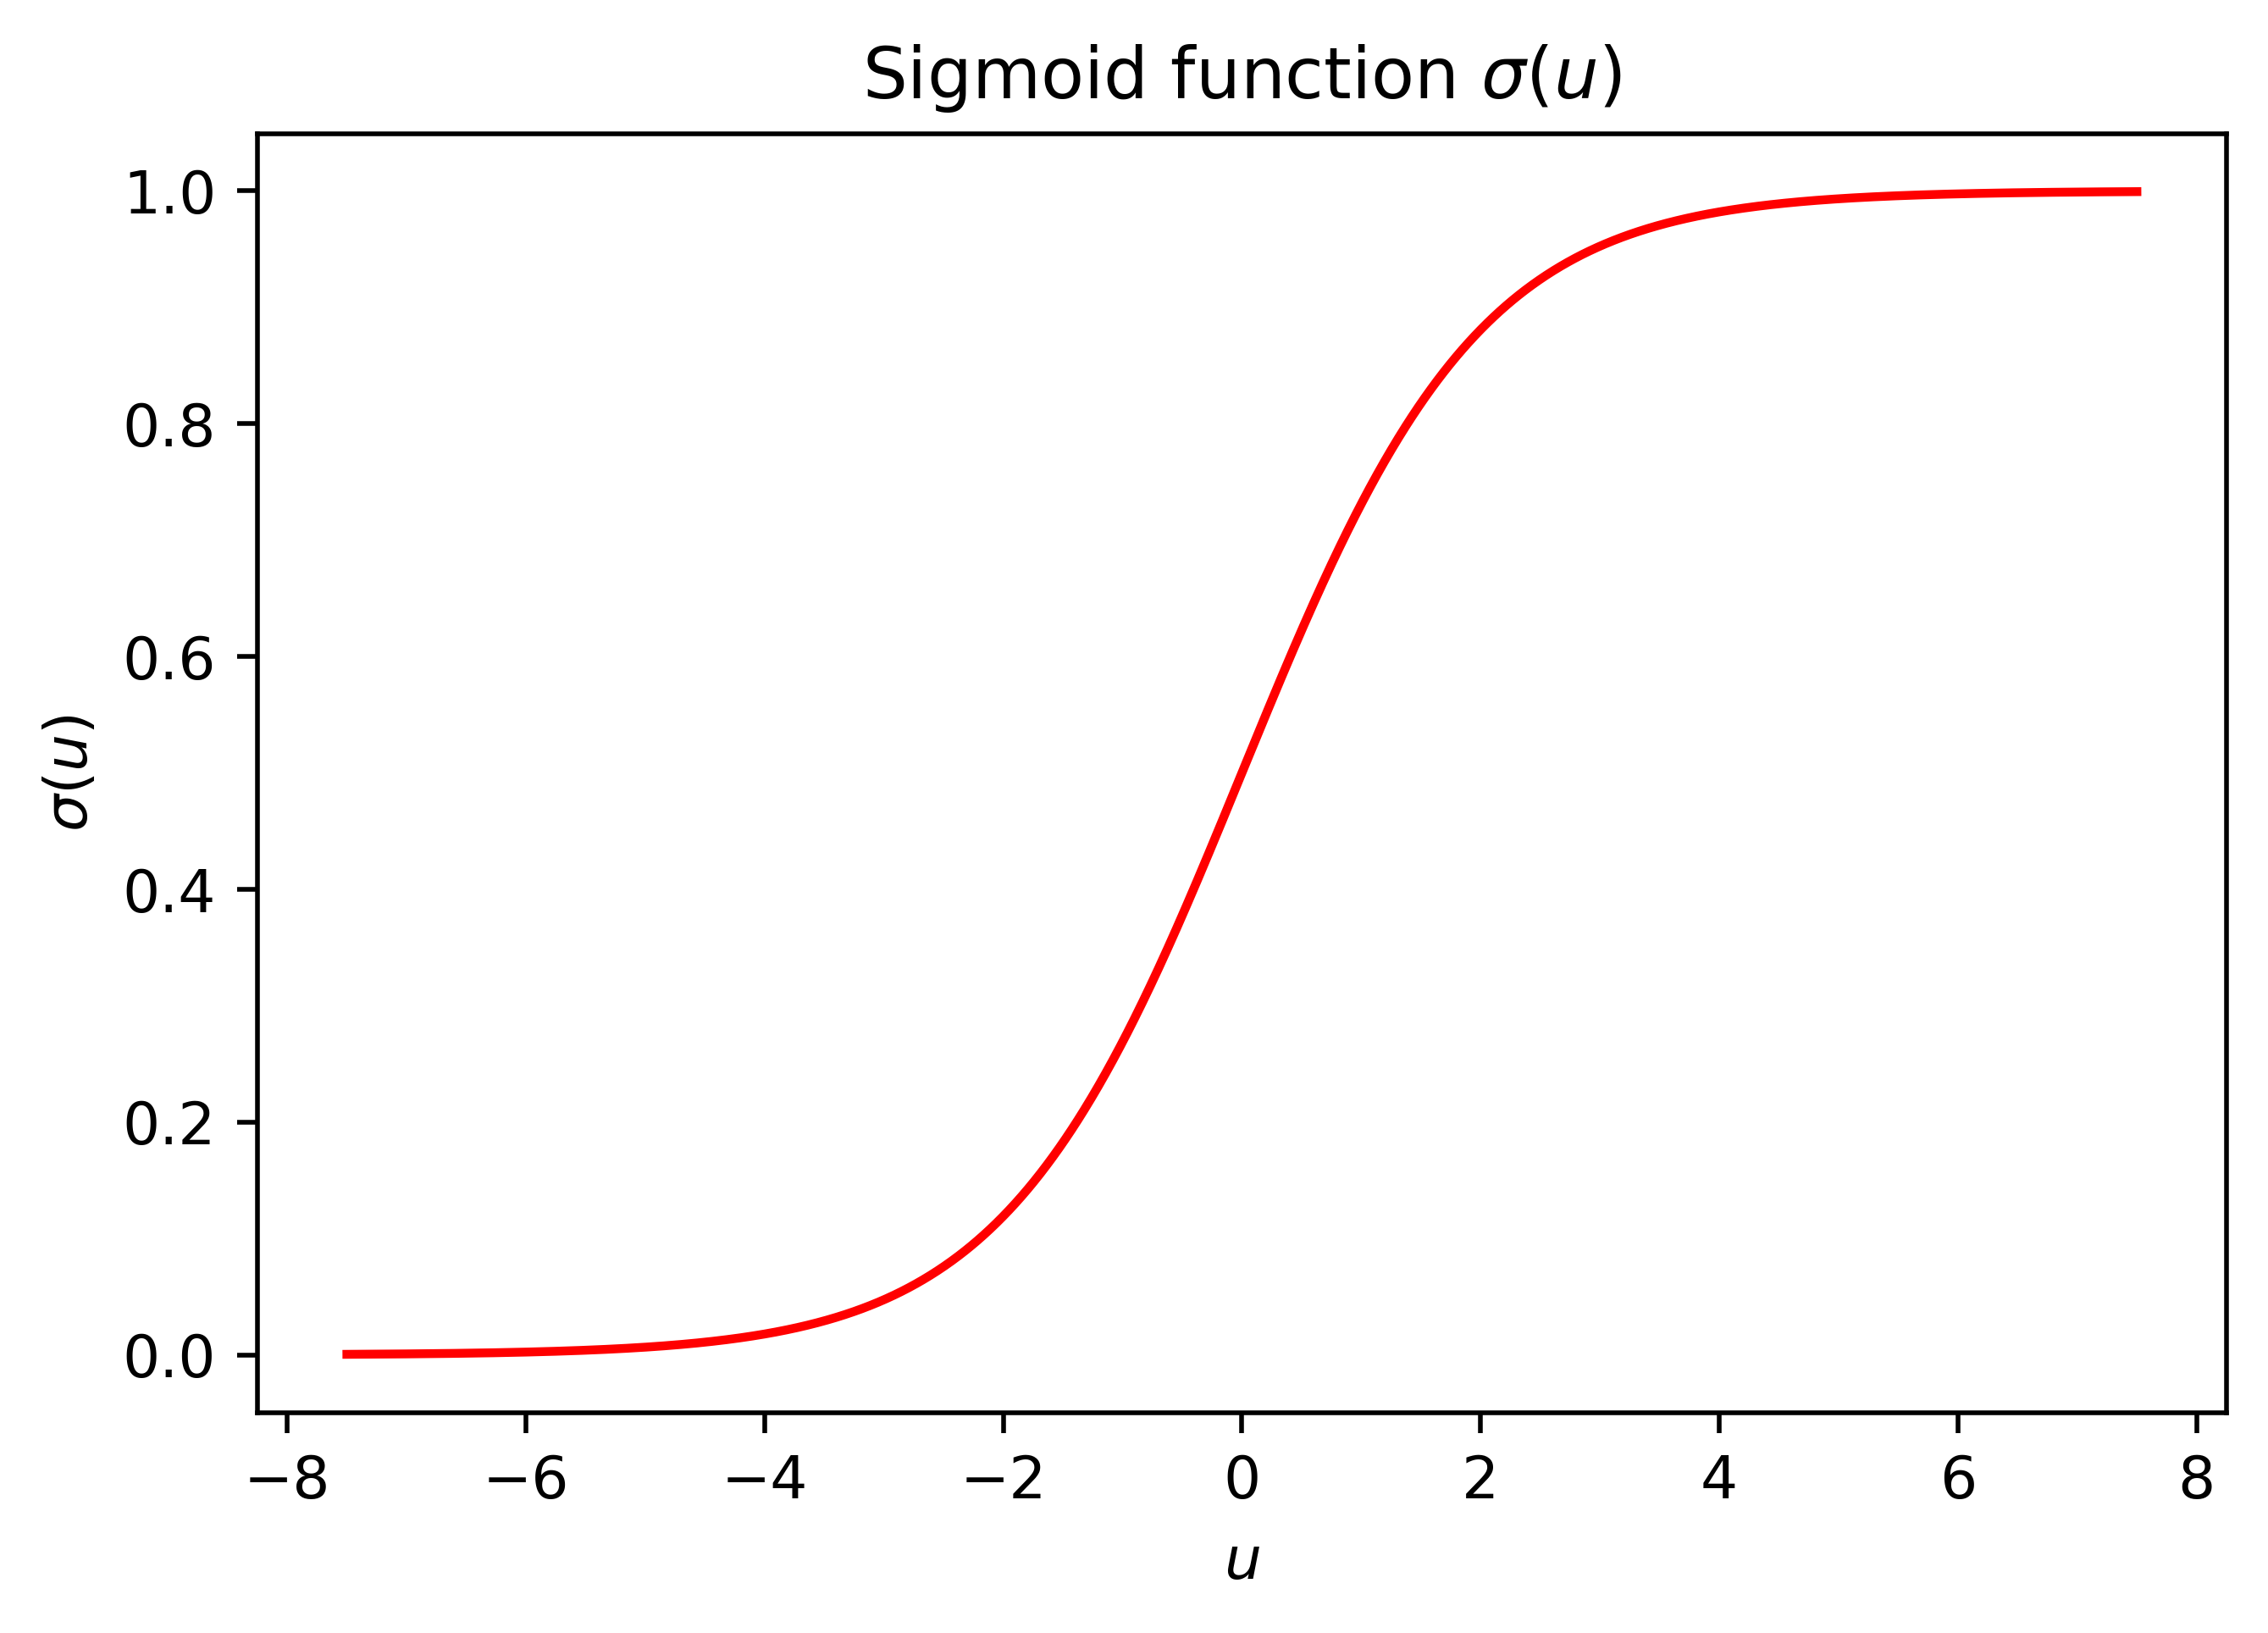
\includegraphics[width=70mm,scale=0.5]{images/classification_images/sigmoid_u.png}
            
            \caption*{$\sigma(u)$ approaches 0 as $u$ approaches $-\infty$, but it never reaches it.}
        \end{figure}
        
        Well, what happens when $u(x)=0$? We get $\sigma(0)=.5$. So, we could use that as our classification: $\sigma(u)>.5$
        
        \begin{figure}[H]
            \centering
            
            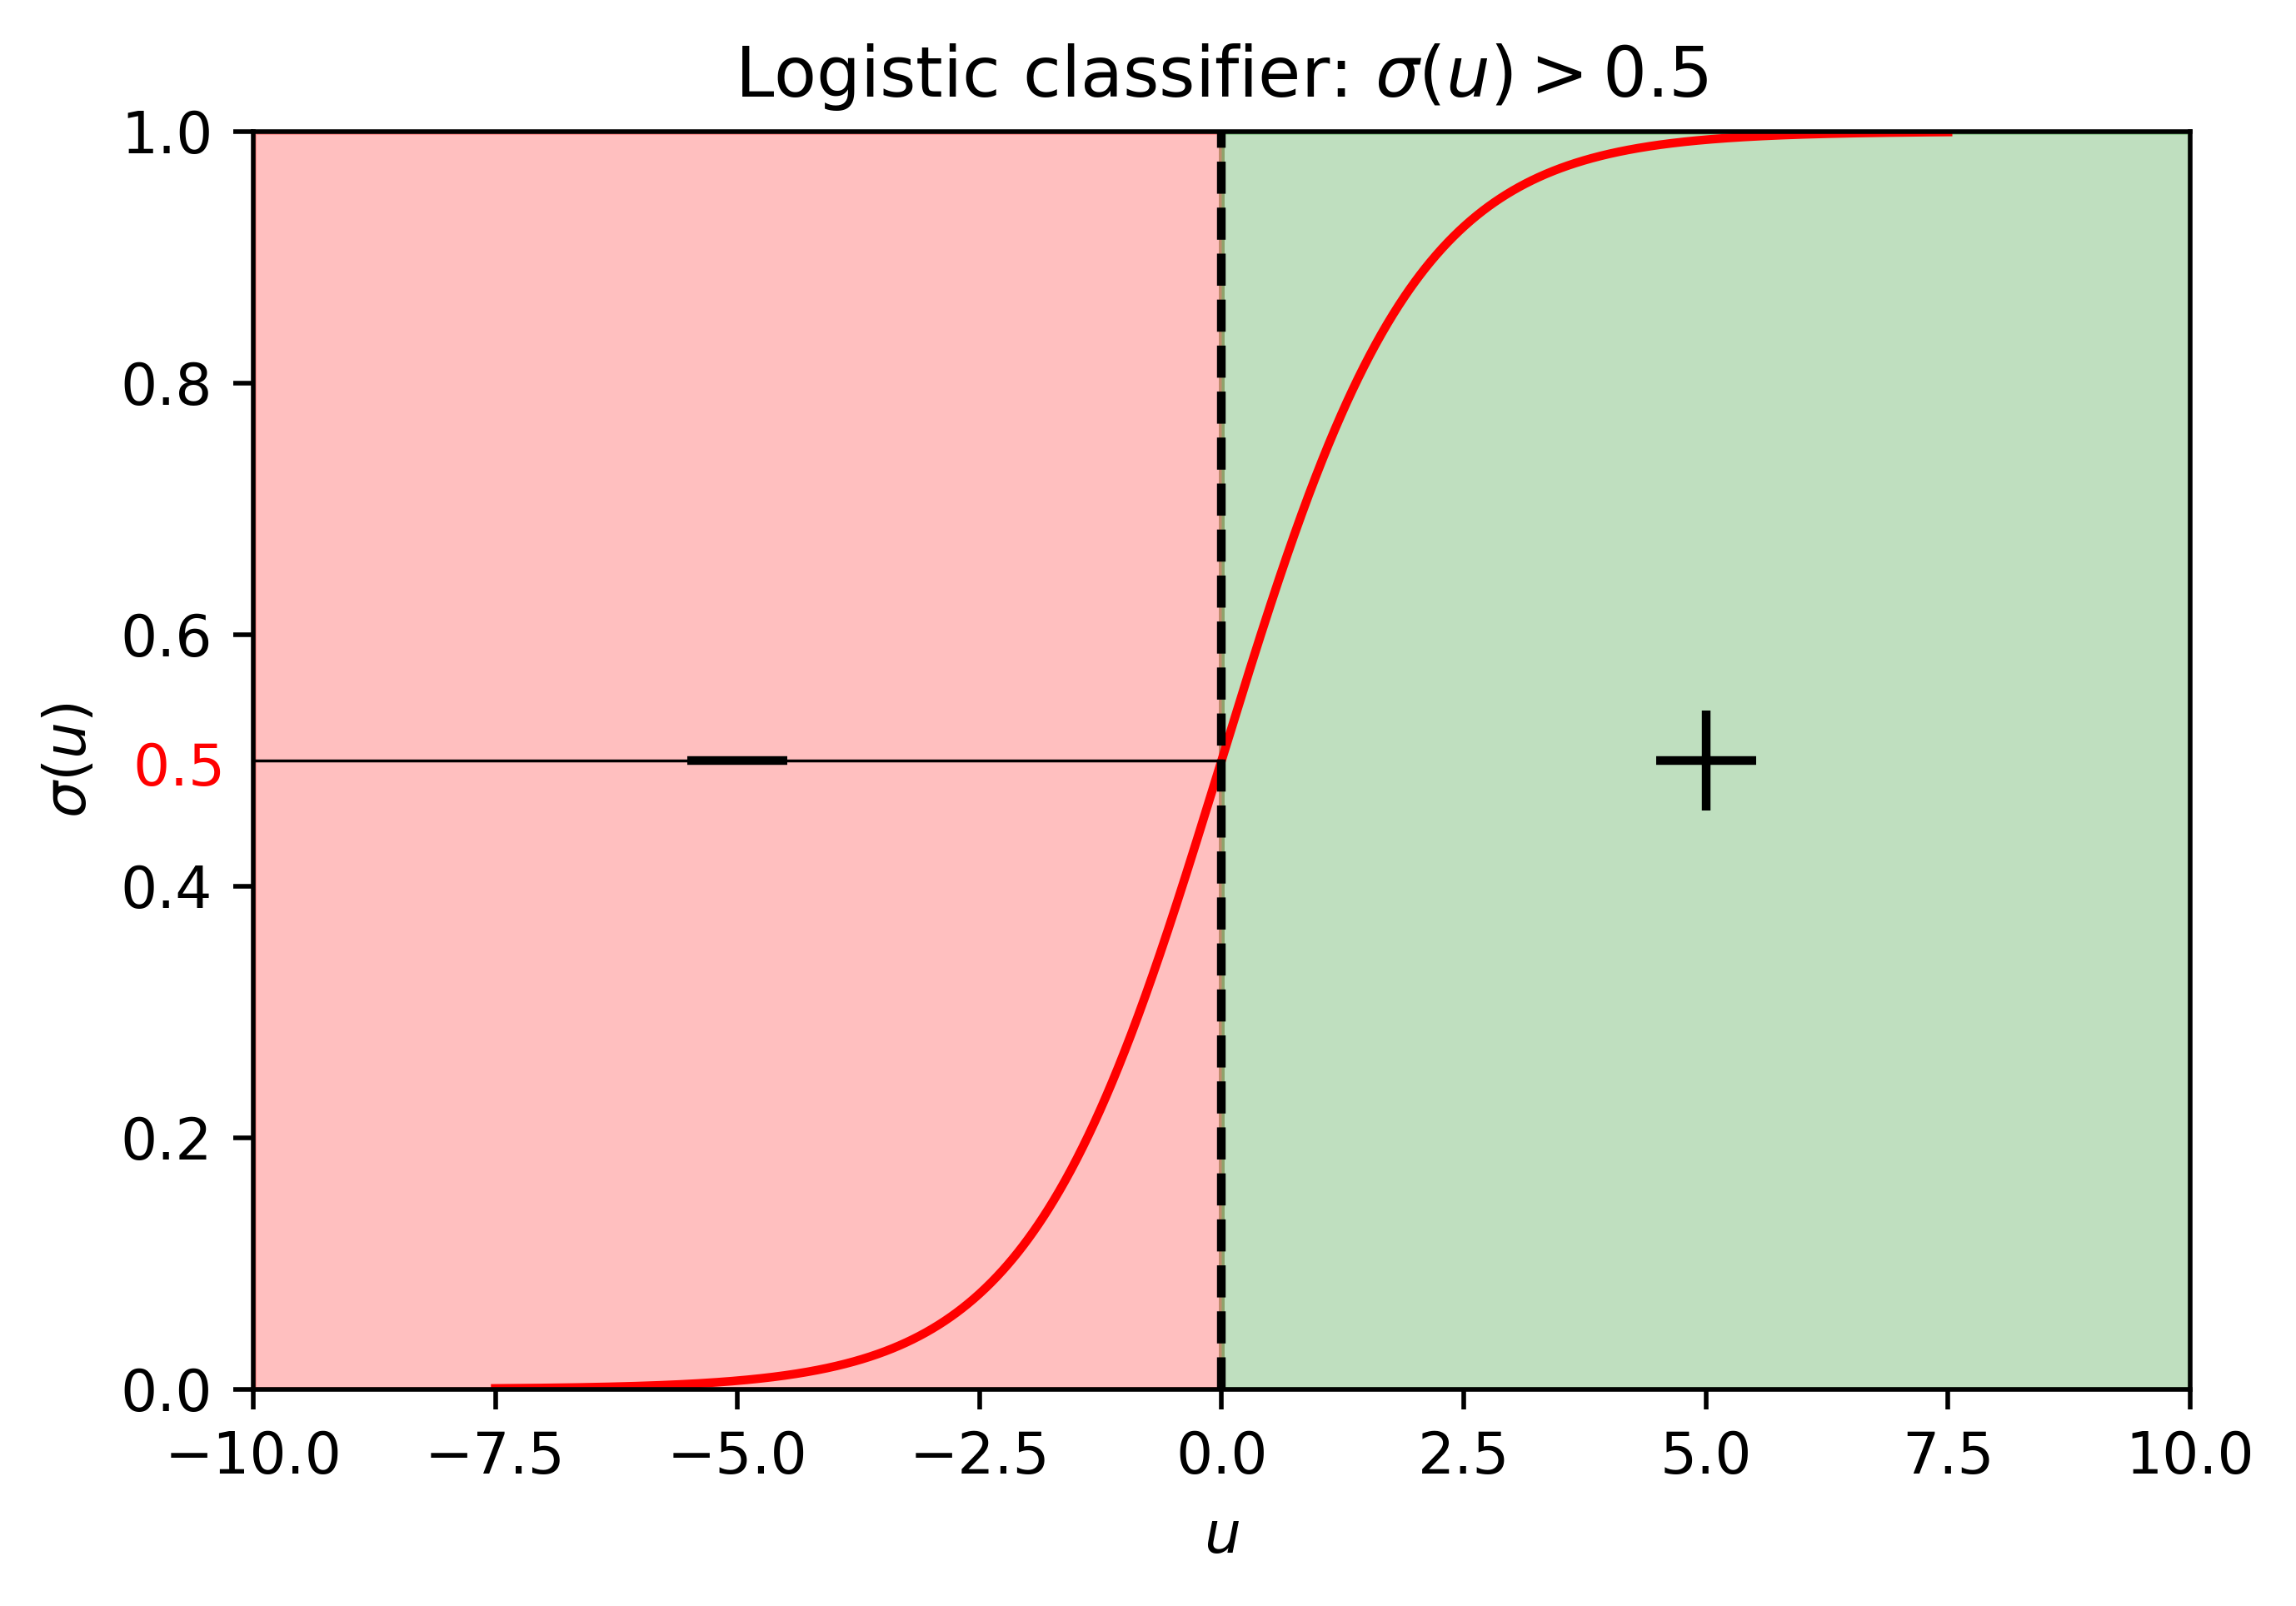
\includegraphics[width=70mm,scale=0.5]{images/classification_images/sigmoid_.5.png}

        \end{figure}
        
        But, we don't necessarily always want to use .5:
        
        \miniex Imagine if you wanted to \textbf{classify} whether someone needs \textbf{life-saving} treatment. Classify $-1$ if sick (they need it), $+1$ if healthy (they don't). 
        
        Let's say you got $\sigma(u)=.6$, so you're only 60\% sure they \textbf{don't} need it. You'd classify that as $\sigma(u)>.5$: they're '\textbf{healthy}'.
        
        Even so, you probably shouldn't \textbf{refuse} someone treatment that's $40\%$ likely to \textbf{save} their life. We might not want to use $\sigma(u)>.5$ after all.
        
        We call the \textbf{boundary} between positive and negative the \textbf{prediction threshold}.\\
        
        \begin{definition}
            The \vocab{prediction threshold} $\sigma_{thresh}$ is the value where you go from \purp{negative} classification to \gren{positive}.
            
            In general, we say
            
            
            
            Our \purp{default} value is a threshold of .5, but our threshold can be \gren{anywhere} in the range
            
            \begin{equation*}
                0 < \sigma_{thresh} < 1
            \end{equation*}
        \end{definition}
        
        \miniex If $\sigma_{thresh}=.9$, we would see:
        
        \begin{figure}[H]
            
            \includegraphics[width=70mm,scale=0.5]{images/classification_images/sigmoid_.5.png}
            \includegraphics[width=70mm,scale=0.5]{images/classification_images/sigmoid_.9.png}
            \caption*{We switch from a .5 threshold to a .9 threshold.}

        \end{figure}
        
    \subsection{Linear Logistic Classifier}
        
        This finally gives us our \textbf{linear logistic classifier} (LLC)\\
        
        \begin{kequation}
            The \vocab{linear logistic classifier} is a \purp{binary} classifier of the form
            
            \begin{equation*}
                h(x; \theta) = 
                \begin{cases}
                    +1 & \text{if $\sigma(\red{u(x)})>\sigma_{thresh}$ }\\
                    -1 & \text{otherwise}
                \end{cases}
            \end{equation*}
            
            where 
            
            \begin{equation}
                u=\theta^T x + \theta_0   \qquad\qquad \sigma(u) = \frac{1}{1+e^{-x}}
            \end{equation}
            
            We call it linear because of the linear inner function $u(x)$, and logistic because of the outer function $\sigma(u)$.
        \end{kequation}
        
    \subsection{Modifying our sigmoid}
    
        What happens when you modify the \textbf{parameters} of an LLC? Let's find out.
        
        We'll use a 1-D input: our variables will be $\theta$ (scalar) and $\theta_0$: $\theta x + \theta_0$
        
        \begin{figure}[H]
            \centering
            \includegraphics[width=70mm,scale=0.5]{images/classification_images/llc_func.png}
            \caption*{Our baseline LLC: $u(x)=1x+0 $}
        \end{figure}
        
        What if we shift by increasing $\theta_0$?
        
        \begin{figure}[H]
            \centering
            \includegraphics[width=70mm,scale=0.5]{images/classification_images/theta_0_+2.png}
            \caption*{Our shifted LLC: $u(x)=1x+4 $. $\theta_0$ shifts us along the $x$-axis!}
        \end{figure}
        
         Just like before, it \textbf{shifts} us in the \textbf{opposite} direction: if $\theta_0$ is \textbf{positive}, we shift in the \textbf{negative} direction, and vice versa.
         
         What if we increase the magnitude of $\theta$!
         
         \begin{figure}[H]
            \centering
            \includegraphics[width=70mm,scale=0.5]{images/classification_images/theta_x4.png}
            \caption*{Our new LLC: $u(x)=4x$. Increasing $\theta$ makes our function steeper!}
        \end{figure}
        
        Making the magnitude of $\theta$ larger makes our function \textbf{change} faster. 
        
        This makes some sense: if $\theta$ (linear slope of $u(x)$) makes $u(x)$ \textbf{change} faster, it will make $\sigma(u)$ change faster \textbf{too}.
        
        You can combine these changes as well: you can shift your LLC with $\theta_0$, and also make it steeper/less steep by changing magnitude of $\theta$.\\
        
        \begin{concept}
            When working with \vocab{sigmoids}, you can \purp{transform} them using your \gren{parameters}:\\
            
            \begin{itemize}
                \item A higher \purp{magnitude} $\norm{\theta}$ makes the slope \gren{steeper}, and answers more \gren{confident}.
                
                \item \purp{Increasing} $\theta_0$ \gren{shifts} the sigmoid in the $-\theta$ \gren{direction}, and vice versa.
            \end{itemize}
        \end{concept}
        
    \subsection{Viewing our sigmoid in 3D}
        
        Let's quickly take a look at a sigmoid in 3D, with two inputs:
        
        \begin{figure}[H]
            \centering
            \includegraphics[width=70mm,scale=0.5]{images/classification_images/llc_3d.png}
        \end{figure}
        
        As you can see, you get mostly the same shape: if you look at it from the side, it's exactly the same, in fact! Just stretched out into 3D.
        
    \subsection{LLCs and overfitting}
    
        In chapter 2, we reduced \textbf{overfitting} by limiting the \textbf{magnitude} of $\theta$ using
        
        \begin{equation}
            R(\theta)=\lambda \norm{\theta}^2
        \end{equation}
        
        In this chapter, it's more clear why reducing \textbf{magnitude} reduces \textbf{overfitting}. Let's see what happens when $\theta$ is very \textbf{large}:
        
        \begin{figure}[H]
            \centering
            \includegraphics[width=70mm,scale=0.5]{images/classification_images/theta_x20.png}
            \caption*{Our shifted LLC: $u(x)=20x$.}
        \end{figure}
        
        This function starts looking more and more like the \textbf{sign} function. This means we very, \textbf{very quickly} go from \textbf{confident} in one answer, to confident in another.
        
        But if you have a limited dataset, and you're very carefully tuned to it, it's doesn't make sense to be \textbf{very confident} in your answer. Especially when you're \textbf{close} to your \textbf{boundary}.
        
        You have closely \textbf{fitted} your sigmoid function to your data: in a way, you may have \textbf{overfitted} it.
        
        The problem is, you're \textbf{rewarded} for increasing $\theta$! If you're just a little bit \textbf{more sure} of the answers you get correct, the loss function continues going \textbf{down}.
        
        So, we need to prevent $\theta$ from \textbf{growing} to an unreasonably high value. We'll \textbf{penalize} a large $\norm{\theta}$.
        
        This means we're \textbf{penalizing} the machine's \textbf{overconfidence} in its answer, so that it \textbf{generalizes} better.\\
        
        \begin{concept}
            In \vocab{classification}, the \vocab{regularizer} follows the form
            
            \begin{equation*}
                R(\theta)=\lambda \norm{\theta}^2
            \end{equation*}
            
            Regularization in this form reduces \purp{overfitting} to our data by
            \begin{itemize}
                \item Making the \textbf{transition} between classifications less \gren{sudden}, when it shouldn't be so \textbf{certain} of the boundary.
                \item It also prevents our model from becoming \purp{overly confident} in its answer.
            \end{itemize} 
        \end{concept}
        
        
        
        
    \subsection{LLCs and LCs have the same boundary}
        
        One more important thing to note: noticed that we set $\sigma_{thresh}=.5$, because that was when $u(x)=0$.
        
        This means that, if our threshold is $0.5$, then the boundary of our LLC should look exactly the same as if it were LC: the only difference is the values that we \textit{can't} see:
        
        \begin{figure}[H]
            \includegraphics[width=70mm,scale=0.5]{images/classification_images/2d_classification_in_3d_plane.png}
            \includegraphics[width=70mm,scale=0.5]{images/classification_images/2d_classification_in_3d_sigmoid.png}
            
            \caption*{Despite having different shapes in 3D, they both create 2-D \textbf{linear} classifiers: on the left, $u(x)=0$, and on the right, $\sigma(u)=.5$.}
        \end{figure}
        
        One way to think about this difference is that while one may be logistic, they are both \textbf{linear}: they both create the same \textbf{linear separator}.
        
        The main benefit of switching to LLC is that $\sigma(u)$ has a useful \textbf{gradient}, while sign$(u)$ does \textbf{not}, so we can do \textbf{gradient descent}.
            \note{The probabilistic interpretation is also more appropriate: we shouldn't be fully confident in our answers.}
            
        Even if we adjust our threshold $\sigma_{thresh}$, that will simply shift the linear classifier.\\
        
        \begin{concept}
            \vocab{LLCs} (Linear Logistic Classifiers) and \vocab{LCs} (Linear Classifiers) both create a \gren{linear} \purp{hyperplane separator} in $d-1$ dimensional \gren{space}.
            
            If the \gren{threshold value} is 0.5, then they have the \purp{exact same} separator.
        \end{concept}
    
    \subsection{Learning LLCs: Loss Functions}
    
        Now that we have fully \textbf{built up} LLCs, we can start trying to \textbf{train} our own. 
        
        In order to do that, we need a way to \textbf{evaluate} our hypotheses: a \textbf{loss function}.
        
        Earlier in the chapter, we tried \textbf{0-1 Loss}:

        \begin{equation*}
            \loss_{01}
            \Big(  
                \red{h(x; \Theta)} ,\quad  y 
            \Big) 
            =
            \begin{cases}
                0 & \text{ if } y = h(x; \Theta)\\
                1 & \text{ otherwise}
            \end{cases}   
        \end{equation*}
        
        But, this \textbf{loss} function the same problem our \textbf{sign} function did: it isn't \textbf{smooth}! 
        
        It's a \textbf{discrete} function based on our \textbf{discrete classes}: so, it won't have a smooth \textbf{gradient} we can do \textbf{descent} on.
        
        For our \textbf{sign} function, we switched to the \textbf{sigmoid} function, which measures in terms of \textbf{probabilities}: this gave us some \textbf{smoothness} to our classification.
        
        Could we do the same here?
        
    \subsection{Building our new loss function}
    
        So, the \textbf{output} of our sigmoid $\sigma(u)$ is a \textbf{probability}: how \textbf{likely} do we think a point is to be in class $+1$?
        
        We want a loss function
        
        \begin{equation}
            \loss(g,y)
        \end{equation}
        
        That considers two facts: the \textbf{correct} answer $y$, and how likely we \textbf{expected} $+1$ to be, $g=\sigma(u)$.\\
        
        \begin{notation}
            For our \vocab{loss function}, rather than using $y \in \{-1,+1\}$, we'll use $ y \in \{0,1\}$.
            
            That way, $\sigma(u)$ and $y$ \purp{match}:
            
            \begin{equation*}
                y \in \{0,1\} \qquad \qquad g \in (0,1)
            \end{equation*}
        \end{notation}
        
        So, if the correct is $1$, then we want $\sigma(u)$ to be \textbf{high}. If the correct answer is $0$, we want $\sigma(u)$ to be \textbf{low}.
        
        For \textbf{one} data point, then, we can consider, "how likely did we think the right answer was?"
        
        \begin{equation}
            G(g,y) = 
            \begin{cases}
                g & \text{if } y=1 \\
                1-g & \text{else } (y=0)
            \end{cases}
        \end{equation}
        
        If we to choose 1 with probability $g$, this could also mean, "how likely were we to be \textbf{right}?"
        
        This $G$ is how "\textbf{good}" our function is, so the \textbf{loss} would need for us to take the \textbf{negative}: we'll do that later.
        
    \subsection{Loss Function for Multiple Data Points}
    
        Now, how do we consider \textbf{multiple} data points? Well, let's think in terms of \textbf{probability}: guessing each point is a separate \textbf{event}.
        
        We \textit{could} add or \textbf{average} our guesses. But, since we're working with \textbf{probabilities}, there's a natural way to \textbf{combine} them: multiple events \textbf{occurring} at the same time.
        
        Before, we asked, "how likely were we to be \textbf{right}?" for \textbf{one} data point. We could \textbf{extend} this question to, "how likely are we to get \textbf{every} question right?"
        
        Well, each question we get right is an \textbf{independent} event $C_i$. If we want two independent events to \textbf{both} happen, we have to \textbf{multiply} their probabilities.\\
        
        \begin{kequation}
            The probability of two independent events $A$ and $B$ happening at the same time is
            
            \begin{equation*}
                \p{A \text{ and } B} = \p{A} * \p{B}
            \end{equation*}
        \end{kequation}

        
        So if we want \textbf{all} of them, we just multiply:
        
        \begin{equation}
            \p{E_{all}} = \p{E_1} * \p{E_2} * ...
            * \p{E_n}
        \end{equation}
        
        Written using pi notation, and also $\ex{g}{i}$ for multiple data points:
            \note{This notation is described in the prerequisites chapter! The short version: instead of adding terms with $\sum$, you multiply with $\prod$.}
            
        \begin{equation}
            \p{E_{all}} = \prod_{i = 1}^n \p{E_i} = \prod_{i = 1}^n \begin{cases}
                \rgi & 
                \text{if } \byi=1 \\
                1-\rgi & 
                \text{if } \byi=0
            \end{cases}
        \end{equation}
        
    \subsection{Simplifying our expression - Piecewise}
        
        Our piecewise function is a bit \textbf{annoying}, though: is there a way to \textbf{simplify} it so that it doesn't have to be \textbf{piecewise}?
        
        Our goal is to \textbf{combine} our two piecewise cases into a \textbf{single} equation. That means one of them needs to \textbf{cancel out} whenever the other is true.
        
        Well, let's see what we have to \textbf{work} with.
        
        Our \textbf{two} cases happen when $y=0$ or $y=1$: these are \textbf{nice} numbers! Why? Because of the \textbf{exponent} rules for these two:
        
        \begin{itemize}
            \item $c^0=1$: an exponent of 0 outputs 1: a factor of 1 in a product might as well \textbf{not be there}. It has been effectively \textbf{cancelled} out.
            
            \item $c^1=c$: an \textbf{exponent} of 1 leaves the factor \textbf{unaffected}.
        \end{itemize}
        
        So, let's consider the \textbf{first} case, $g$. we can use $\red{g}^{ \blu{y} }$: if $y=1$, it's \textbf{unaffected}. If $y=0$, the term is \textbf{removed}.
        
        We want the \textbf{opposite} for $1-g$. We can \textbf{swap} 1 and 0 by doing $1-y$. This gives us $(1-\red{g})^{ 1-\blu{y} }$.
        
        For one data point:
        
        \begin{equation}
            \p{E} = 
            \overbrace{
                \red{g} ^ { \blu{y} } 
            }^{y=1}
            \overbrace{
                \left( 
                    1-\red{g} 
                \right) 
                ^ { 1-\blu{y} }
            }^{y=0}
        \end{equation}
        
        We've gotten rid of the piecewise function! Let's add back in the product:
        
        \begin{equation}
            \p{E_{all}} = 
            \prod_{i = 1}^n
            \p{E_i}
            =
            \prod_{i = 1}^n
            \rgi ^ {\byi}
            \left( 
                1-\rgi 
            \right) 
            ^ { 1 - \byi }
        \end{equation}
        
        Looks pretty ugly, but we'll work on that.
        
    \subsection{Getting rid of the product}
    
        Our exponents look pretty \textbf{ugly}. Can we do something about that?
        
        More importantly, \textbf{products} are also pretty unpleasant: we can't use \textbf{linearity}! 
            \note{Linearity makes lots of problems easy to work with, so we try to keep it.}
        
        Linearity uses \textbf{addition} between variables. What sort of \textbf{function} could change a \textbf{product} into a \textbf{sum}?
        
        Well, we could \textbf{list} out different basic functions, to see which ones connect sums and products. It turns out, one \textbf{interesting} function is
        
        \begin{equation}
            \overbrace{
                \log{ab}}
            ^{product}
            =
            \overbrace{
                \log{a} + \log{b}
            }^{sum}
        \end{equation}
        
        Aha! If we take the \textbf{log} of our function, we can turn a \textbf{product} into the \textbf{sum}!
            \note{The below equation looks complicated, but all we've done is swap the product for a sum!}

        \begin{equation}
            \overbrace{
                \pur{\log}
                \left(
                    \pur{\prod_{i = 1}^n}
                    \p{E_i}
                \right)
            }^{product}
            =
            \overbrace{
                \pur{\sum_{i = 1}^n
                \log}
                \left(
                    \p{E_i}
                \right)
            }^{sum}
        \end{equation}
        
        We can also separate our two \textbf{factors}:
        \begin{equation}
            \sum_{i = 1}^n
            \Bigg(
                \log\left(
                        \rgi ^{\byi}
                \right)
                \pur{+}
                \log\left( 
                    \left(  1 - \rgi  \right)
                    ^ { 1 - \byi }
                \right) 
            \Bigg)
        \end{equation}
        
        And \textbf{finally}, we can remove the \textbf{exponents}:
        
        \begin{equation}
            \sum_{i = 1}^n
            \Bigg(
                \byi\log{\rgi}
                +
                \left( 1 - \byi \right)
                \log
                    \left( 1 - \rgi \right) 
            \Bigg)
        \end{equation}
    
        \begin{concept}
            Our \vocab{negative log likelihood} (NLL) comes from a couple steps:
            
            \begin{itemize}
                \item \purp{Use} $y \in \{0, 1\}$ instead of $y \in \{-1,+1\}$ so that $y$ and $g$ have \gren{matching} outcomes.
            
                \item Get the \purp{chance} the model is right on every \gren{guess}: a \gren{product}.
                
                \item Use \purp{exponents} to convert the \gren{piecewise} expression into a single \gren{equation}.
                
                \item Take the \purp{log} of our expression to switch from a \gren{product} to a \gren{sum}.
                
                \item Take the \purp{negative} to get the \gren{loss} rather than the "\gren{goodness}" of our function.
            \end{itemize}
        \end{concept}    
        
    \subsection{Negative Log Likelihood}
    
        Remember, at the \textbf{beginning}, we said that we need to take the \textbf{negative}: our function represents how \textbf{good} our function is, but we want the \textbf{loss}.
        
        With this, our function is in its final form:\\
        
        \begin{kequation}
            We can get the loss of our \vocab{linear logistic classifier (LLC)} using the \vocab{negative log likelihood (NLL)} loss function
            
            \begin{equation*}
                \loss_{nll}
                (\rgi ,\quad \byi)
                =
                -
                \Bigg(
                    \byi \log{\rgi}
                    +
                    \left( 1 - \byi \right)
                    \log
                    \left( 1-\rgi \right) 
                \Bigg)
            \end{equation*}
            
            Or,
            
            \begin{equation*}
                -
                \Big(
                    (\blu{answer}) \log(\red{guess})
                    +
                    \left( 1 - \blu{answer} \right)
                    \log
                    \left( 1-\red{guess} \right) 
                \Big)
            \end{equation*}
        \end{kequation}
        
        Our total loss is
        
        \begin{equation}
            \sum_{i=1}^n 
            \loss_{nll}(\rgi ,\quad \byi)
        \end{equation}
        
        Finally, we add our \textbf{regularizer}:
        
        \begin{equation}
            J_{lr}(\theta,\theta_0;\data)
            =
            \frac{1}{n} \sum_{i=1}^n 
            \Big(
                \loss_{nll}(\rgi ,\quad \quad \byi)
            \Big)
            +
            \pur{ \lambda \norm{\theta}^2 }
        \end{equation}
        
        \begin{kequation}
            The full \vocab{objective function} for \vocab{LLC} is given as
            
            \begin{equation*}
                J_{lr}(\theta,\theta_0;\data)
                =
                \frac{1}{n}
                \sum_{i=1}^n 
                \Bigg(
                    \loss_{nll}
                    \left(
                        \red{\sigma(\theta^T x + \theta_0)} ,\quad \byi
                    \right)
                \Bigg)
                +
                \pur{ \lambda \norm{\theta}^2 }
            \end{equation*}
            
            Using our \purp{loss} function $\loss_{nll}$, and our \purp{logistic} function $\sigma(u)$.
            
        \end{kequation}

\pagebreak
%%%%%%%%%%%%%%%%%%%%%%%%%%%%%%%%%%%%%%%%%%%%%%%%%%%%%%%%%%%%%%%%%%%%%%%%%%%%%

\section{Gradient Descent for Logistic Regression}

    \subsection{Summary}
    
    Now, we have developed all the tool we need to do binary classification with LLC:
    
    \begin{itemize}
        \item A \textbf{linear} model that lets us \textbf{combine} our variables,
            \begin{equation}
                u(x) = \theta^T x + \theta_0
            \end{equation}
            
        \item A \textbf{logistic} model that lets us get the \textbf{probability} of a classification,
            \begin{equation}
                \sigma(u) = \frac{1}{1+e^{-u}}
            \end{equation}
            
        \item A \textbf{threshold value} we use to determine how to \textbf{classify} our data,
            \begin{equation}
                h(x; \theta) = 
                \begin{cases}
                    +1 & \text{if $\sigma(\red{u(x)})>\sigma_{thresh}$ }\\
                    0 & \text{otherwise}
                \end{cases}
            \end{equation}
            
        \item A \textbf{loss function} NLL we use to \textbf{evaluate} our model performance:
        
            \begin{equation*}
                \loss_{nll}
                (\rgi ,\quad \byi)
                =
                -
                \left(
                    \byi \log{\rgi}
                    +
                    \left( 1 - \byi \right)
                    \log
                    \left( 1-\rgi \right) 
                \right)
            \end{equation*}
            
        \item And an \textbf{objective function} we can \textbf{optimize}:
        
            \begin{equation}
                J_{lr}(\theta,\theta_0;\data)
                =
                \pur{ \lambda \norm{\theta}^2 }
                +
                \frac{1}{n} \sum_{i=1}^n 
                    \loss_{nll}(\rgi ,\quad \byi)
            \end{equation}
    \end{itemize}
    
    We have everything we need to do optimization.
    
    \subsection{The problem: Gradient Descent}
    
        We want to do \textbf{gradient descent} to minimize $J_{lr}$
        
        \begin{equation}
            \pur{ R(\theta) }
            +
            J_{lr}(\theta,\theta_0)
            =
            \frac{1}{n}
            \sum_{i=1}^n 
            \loss_{nll}(\rgi ,\quad \byi)
        \end{equation}
        
        We want repeatedly \textbf{adjust} our model $\Theta=(\theta,\theta_0)$ to improve $J_{lr}$. To do that, we want the gradients for $\theta$ and $\theta_0$. Let's start with $\theta$.
        
        \begin{equation}
            \nabla_\theta J_{lr} = \pderiv{J_{lr}}{\theta}
        \end{equation}
        
        First, $J_{lr}$ has \textbf{two} terms, so we'll separate them.
        
        \begin{equation}
            \nabla_\theta J_{lr} = 
            \pderiv{R}{\theta} + \frac{1}{n} \sum_{i=1}^{n }
                \pderiv{\loss_{NLL}}{\theta} (\rgi ,\quad \byi)
        \end{equation}
        
        The regularization term is pretty easy, because we did it last chapter:
        
        \begin{equation}
            \pderiv{R}{\theta} = 2 \lambda \theta
        \end{equation}
        
        But what about our first term?
    
    \subsection{Getting the gradient: Chain Rule}
    
        Now, we just need to do
        
        \begin{equation}
            \pderiv{\loss_{NLL}}{\theta} (\red{g} , \blu{y})
        \end{equation}
    
        With our $\loss_{NLL}$ term, we run into an issue: how do we take the \textbf{derivative}? The function is very, very deeply \textbf{nested}. In our case: 
        
        $x$ \textbf{affects} $u(x)$. $u(x)$ \textbf{affects} $\sigma(u)$. $\sigma(u)=g$ \textbf{affects} $\loss_{NLL}(g,y)$, which finally \textbf{affects} $J(\theta,\theta_0)$. 
        
        How do we represent this \textbf{chain} of functions? With the \textbf{chain rule}:
        
        \begin{equation}
            \pderiv{A}{C} = \pderiv{A}{B} \cdot \pderiv{B}{C}
        \end{equation}
        
        So, we'll build up a \textbf{chain rule} for our needs. We'll use $g=\sigma(u)$.
        
        \begin{equation}
            \pderiv{ \loss_{NLL} }{ \theta } 
            = 
            \pderiv{ \loss_{NLL} }{\blu{\sigma}} 
            \cdot 
            \pderiv{\blu{\sigma}}{\theta}
        \end{equation}
        
        Sigma contains $u$, so we'll use that instead:

        \begin{equation}
            \pderiv{ \loss_{NLL} }{ \theta } 
            = 
            \pderiv{ \loss_{NLL} }{ \blu{\sigma} } 
            \cdot 
            \pderiv{ \blu{\sigma} }{\red{u}} 
            \cdot 
            \pderiv{\red{u}}{\theta}
        \end{equation}
        
        This is our full \textbf{chain rule}!\\
        
        \begin{kequation}
            The \vocab{gradient} of \vocab{NLL} can be calculated using the \purp{chain rule}:
            
            \begin{equation}
                \pderiv{ \loss_{NLL} }{ \theta } 
                = 
                \pderiv{ \loss_{NLL} }{\blu{\sigma}} 
                \cdot 
                \pderiv{ \blu{\sigma} }{\red{u}} 
                \cdot 
                \pderiv{\red{u}}{\theta}
            \end{equation}
        \end{kequation}
        
    \subsection{Getting our individual derivatives}
    
        We can take the derivative of each of these objects. First, let's look at $\loss_{NLL}$
        
        \begin{equation*}
            \loss_{nll}
            (\red{\sigma}, \blu{y})
            =
            -
            \Big(
                \blu{y} \log{ \red{\sigma} }
                +
                \left( 1 - \blu{y} \right)
                \log
                \left( 1 - \red{\sigma} \right) 
            \Big)
        \end{equation*}
        
        And we'll use $\deriv{}{x} log(x) = \frac{1}{x}$
        
        \begin{equation}
        \boxed{
            \pderiv{ \loss_{NLL} }{\red{\sigma}} =
            -
            \Big(
                \frac{ \blu{y} } { \red{\sigma} } 
                -
                \frac{ 1-\blu{y} } { 1 - \red{\sigma} }
            \Big)
        }
        \end{equation}
        
        Now, we look at $\sigma(u)$:
        
        \begin{equation}
            \sigma(\blu{u}) = \frac{1}{1+e^{-\blu{u} }}
        \end{equation}
        
        If we take the derivative, we can get:
        
        \begin{equation}
            \pderiv{ \blu{\sigma} }{\red{u}}
            =
            \frac{ -e^{ -\blu{u} } }{ \Big(   1+e^{ -\blu{u} }   \Big)^2 }
        \end{equation}
        
        Which we can rewrite, conveniently, as
            \note{Try this yourself if you're curious!}
        
        \begin{equation}
        \boxed{
            \pderiv{ \blu{\sigma} }{\red{u}}
            =
            \sigma (1-\sigma)
        }
        \end{equation}
        
        Finally, our last derivative:
        
        \begin{equation}
            u = \theta^Tx+\theta_0
        \end{equation}
        
        \begin{equation}
        \boxed{
            \pderiv{\red{u}}{\theta} = x
        }
        \end{equation}
        
    \subsection{Simplifying our chain rule}
    
        So, now, we can put together our chain rule:
        
        \begin{equation}
            \pderiv{ \loss_{NLL} }{ \theta } 
            = 
            \pderiv{ \loss_{NLL} }{ \blu{\sigma} } 
            \cdot 
            \pderiv{ \blu{\sigma} }{\red{u}} 
            \cdot 
            \pderiv{\red{u}}{\theta}
        \end{equation}
        
        Plug in the derivatives:
        
        \begin{equation}
            \pderiv{ \loss_{NLL} }{ \theta } 
            = 
            -
            \Big(
                \frac{ \blu{y} } { \red{\sigma} } 
                -
                \frac{ 1-\blu{y} } { 1 - \red{\sigma} }
            \Big)
            \cdot
            \red{\sigma} (1-\red{\sigma})
            \cdot 
            x
        \end{equation}
        
        Simplify:
        
        \begin{equation}
            \pderiv{ \loss_{NLL} }{ \theta } 
            = 
            \Big(
                (1-\blu{y})\red{\sigma} 
                -
                \blu{y}(1-\red{\sigma})
            \Big)
            \cdot 
            x
        \end{equation}
        
        And finally, we sum the terms. We can do the $\theta_0$ gradient at the same time: the only difference is that $\pderiv{u}{\theta_0}=1$, instead of x.\\
        
        \begin{kequation}
            The \vocab{gradients} of NLL for gradient descent are
            
            \begin{equation*}
                \nabla_\theta \loss_{NLL} 
                =
                (\red{\sigma} - \blu{y})x
            \end{equation*}
            
            \begin{equation*}
                \pderiv{\loss_{NLL}}{\theta_0}
                =
                (\red{\sigma} - \blu{y})
            \end{equation*}
        \end{kequation}
        
        We can plug this into $J_{lr}$:
            \note{One comment we didn't make: remember that $R(\theta)$ won't show up in the $\theta_0$ derivative!}
        
        \begin{equation}
            \nabla_\theta J_{lr} 
            =
            \frac{1}{n} \sum_{i=1}^{n }
            \Bigg(
                \Big(\rgi - \byi \Big) \ex{x}{i}
            \Bigg)
            +
            \pur{ 2 \lambda \theta }
        \end{equation}
        
        \begin{equation}
            \pderiv{J_{lr}}{\theta_0}
            =
            \frac{1}{n} \sum_{i=1}^{n } \left( \rgi - \byi \right)
        \end{equation}
        
        We can use this to do \textbf{gradient descent}!
        
        \begin{equation}
            \red{ \theta_{new} } = \blu{ \theta_{old} } - \grn{\eta} \nabla_\theta J_{lr} (\blu{ \theta_{old} })
        \end{equation}
        
        In $\ex{\theta}{t}$ notation:
        
        \begin{equation}
            \red{ \ex{\theta}{t} } = \blu{ \ex{\theta}{t-1} } - \grn{\eta} 
            \left(
            \nabla_\theta J_{lr} (\blu{ \ex{\theta}{t-1} })
            \right)
        \end{equation}
        
        \begin{equation}
            \red{ \ex{\theta_0}{t} } = \blu{ \ex{\theta_0}{t-1} } - \grn{\eta} 
            \left(
                \pderiv{ J_{lr} (\blu{ \ex{\theta}{t-1} })}{\theta_0}
            \right)
        \end{equation}
        
        This also corresponds to some basic math within Neural Networks, which we will return to \textbf{later} in the course.

\pagebreak
%%%%%%%%%%%%%%%%%%%%%%%%%%%%%%%%%%%%%%%%%%%%%%%%%%%%%%%%%%%%%%%%%%%%%%%%%%%%%

\section{Handling Multiple Classes}

    Now, we have developed a \textbf{binary} classifier, using logistic regression. But, many (almost all) problems have more than two classes! 
    
    \miniex Different animals, genres of movies, sub-types of disease, etc.
    
    \subsection{Approaches to multi-class classification}
        
        So, we need to a way to do \textbf{multi-classing}. Consider two main approaches:
        
        \begin{itemize}
            \item \textbf{Train} many binary classifiers on different \textbf{classes} and \textbf{combine} them into a single model.
                \begin{itemize}
                    \item There are several ways to \textbf{combine} these \textbf{classifiers}. We won't go over them here, but some \textbf{names}: OVO (one-versus-one), OVA (one-versus-all).
                \end{itemize}
                
            \item \textbf Make \textbf{one} classifier that handles the multi-class problem by itself. 
                \begin{itemize}
                    \item This model will be A \textbf{modified} version of logistic regression, using a variant of NLL.
                \end{itemize}
    \end{itemize}
    
    The \textbf{latter} approach is what we will use in this \textbf{next} section.
    
    \subsection{Extending our Approach: One-Hot Encoding}
    
        Rather than being \textbf{restricted} to classes 0 and 1, we'll have $k$ \textbf{distinct} classes. Our \textbf{hypothesis} will be
        
        \begin{equation*}
            h: \RR^d \rightarrow \{C_1, C_2, C_3, \dots C_k\}
        \end{equation*}
        
        Where $C_i$ is the $\nth{i}$ class. Meaning, we want to \textbf{output} one of those $k$ \textbf{classes}.
        
        Because we'll be using our computer to do \textbf{math} to get the \textbf{answer}, we need to represent this with \textbf{numbers}. Before, we would simply \textbf{label} with 0 or 1. 
        
        We could return $\{1,2,3,4,5...k\}$ for each \textbf{label}. But this is \textbf{not} a good idea: it implies that there's a natural \textbf{order} to the classes, which isn't necessarily true.
        
        If we don't \textbf{actually} think $C_1$ is closer to $C_2$ than to $C_5$, we probably shouldn't represent them with numbers that are \textbf{closer} to each other.
        
        Instead, each class needs to be a \textbf{separate} variable. We can store them in a vector:
        
        \begin{equation}
            \begin{bmatrix}
              C_1\\C_2\\ \vdots \\ C_k
            \end{bmatrix}
        \end{equation}
        
        So, our \textbf{label} will be
        
        \begin{equation}
            y=
            \begin{bmatrix}
              y_1\\y_2\\ \vdots \\ y_k
            \end{bmatrix}
        \end{equation}
        
        In binary classification, we used 0 or 1 to indicate whether we fit into one \textbf{class}. So, that's how we'll do each class: 0 if our data point is \textbf{not} in this class, 1 if it \textbf{is}.
        
        This approach is called \textbf{one-hot encoding}.\\
        
        \begin{definition}
            \vocab{One-hot encoding} is a way to represent \vocab{discrete} information about a data point.
            
            Our $k$ classes are stored in a length-$k$ column \gren{vector}. For \purp{each} variable in the vector, 
            
            \begin{itemize}
                \item The value is \gren{0} if our data point is \purp{not in that class}.
                \item The value is \gren{1} if our data point is \purp{in that class}.
            \end{itemize}
            
            In one-hot encoding, items are \purp{never} labelled as being in \purp{two} classes at the \gren{same time}.
        \end{definition}
        
        \miniex Suppose that we want to classify \textbf{furniture} as table, bed, couch, or chair.
        
        \begin{equation}
            \begin{bmatrix}
              \text{table} \\ \text{bed} \\ \text{couch} \\ \text{chair} 
            \end{bmatrix}
        \end{equation}
        
        For each class:
        
        \begin{equation}
            y_{chair} = 
            \begin{bmatrix}
              0\\0\\0\\1
            \end{bmatrix}
            \qquad
            y_{table} = 
            \begin{bmatrix}
              1\\0\\0\\0
            \end{bmatrix}
            \qquad
            y_{couch} = 
            \begin{bmatrix}
              0\\0\\1\\0
            \end{bmatrix}
            \qquad
            y_{bed} = 
            \begin{bmatrix}
              0\\1\\0\\0
            \end{bmatrix}
        \end{equation}
        
    \subsection{Probabilities in multi-class}
    
        So, we now know our \textbf{problem}: we're taking in a data point $x \in \RR^d$, and \textbf{outputting} one of the classes as a \textbf{one-hot vector}.
        
        So, now that we know what sorts of data we're \textbf{expecting}, we need to decide on the formats of our \textbf{answer}.
        
        We'll be returning a vector of length-$k$: \textbf{one} for each \textbf{class}. When we were doing \textbf{binary} classification, we estimated the \textbf{probability} of the positive class.
        
        So, it should make sense to do the same \textbf{here}: for each class, we'll return the estimated \textbf{probability} of our data point being in that class.
        
        \begin{equation}
            g
            =
            \begin{bmatrix}
              \p{x \text{ in } C_1} \\ 
              \p{x \text{ in } C_2} \\ 
              \vdots \\ 
              \p{x \text{ in } C_k} 
            \end{bmatrix}
            =
            \begin{bmatrix}
              g_1\\g_2\\\vdots\\g_k
            \end{bmatrix}
        \end{equation}
        
        We can add an \textbf{additional} rule: the probabilities need to add up to \textbf{one}: we should assume our point ends up in some class or \textbf{another}.
        
        \begin{equation}
            g_1+g_2+...+g_k=1
        \end{equation}
        
        \begin{concept}
            The different terms of our \vocab{multi-class} guess $g_i$ represent the \purp{probability} of our data point being in class $C_i$.
            
            Because we should assume our data point is in \purp{some} class, all of these probabilities have to \gren{add} to 1.
        \end{concept}
        
        \textbf{Scaling} values to add up to 1 is called \textbf{normalization}. How do we do that?
        
        Well, let's say each class gets a \textbf{value} of $r_i$, before being \textbf{normalized}: we have done some other math we won't worry about.
        
        To make the total 1, we'll \textbf{scale} our terms by a factor $C$:
        
        \begin{equation}
            C(r_1+r_2+...r_k) 
            = 
            C \left(\sum_{i=1}^k r_i \right)
            =
            1  
        \end{equation}
        
        We can get our factor $C$ just by dividing:
        
        \begin{equation}
            C 
            =
            \frac{1}{\sum r_i}
        \end{equation}
        
        We've got $g_i$ now!
        
        \begin{equation}
            g = 
            \begin{bmatrix}
                r_1/\sum r_i  \\
                r_2/\sum r_i  \\
                \vdots  \\
                r_k/\sum r_i  \\
            \end{bmatrix}
        \end{equation}
        
    \subsection{Turning sigmoid multi-class}
    
        Now, we just need to compute $r_i$ terms to plug in. To do that, we'll see how we did it using sigmoid:
        
        \begin{equation}
            g= \sigma(u) = \frac{1}{1+e^{-u}}
        \end{equation}
        
        This function is 0 to 1, which is good for being a probability. 
        
        Just for our convenience, we'll switch to positive exponents: all we have to do is multiply by $e^u/e^u$.
            \note{Negative numbers are easy to mess up in algebra.}
        
        \begin{equation}
            g = \frac{e^u}{1+e^u}
        \end{equation}
        
        We'll think of \textbf{binary} classification as a special case of \textbf{multi-class} classification. The above probability could be thought of as $g_1$: the chance of our first class.\\
        
        \begin{concept}
            \vocab{Binary classification} is a \purp{special} case of \vocab{multi-class} classification with only \gren{two} classes. 
            
            So, we can use it to figure out the \purp{general} case.
        \end{concept}
        
        So, what was our \textbf{second} probability, $1-g$? This will be our second class, $g_2$.
        
        \begin{equation}
            g_2 = 1-g= \frac{1}{1+e^{u}}
        \end{equation}
        
        This follows an $r_i/(\sum r_i)$ format: the numerators (1 and $e^u$) add to \textbf{equal} the denominator ($1+e^u$).
        
        \begin{equation}
            g = 
            \begin{bmatrix}
                1/(1+e^u)  \\
                e^u/(1+e^u)  \\
            \end{bmatrix}
        \end{equation}
        
        How do we \textbf{extend} this to \textbf{more} classes? Well, 1 and $e^u$ are \textbf{different} functions: this a problem. We want to be able to \textbf{generalize} to many $r_i$. 
        
        How do they make them \textbf{equivalent}? We could say $1=e^0$. So, we could treat both terms as \textbf{exponentials}!
        
        \begin{equation}
            g_1 = \frac{e^u}{e^0+e^u}
        \end{equation}
        
        We can do this for an \textbf{arbitrary} number of terms. We'll treat them as \textbf{exponentials}, just like for $e^u$ and $e^0$
        
        \begin{equation}
             g_i 
            =             \frac{r_i}{\sum r_j} 
            = 
            \frac{e^{u_i}}{\sum e^{u_j}}
        \end{equation}
        
    \subsection{Our Linear Classifiers}
    
        What are each of those $u_i$ terms? When we were doing \textbf{binary}, it was a \textbf{linear regression} function:
        
        \begin{equation}
            u(x) = \theta^Tx+\theta_0
        \end{equation}
        
        We can do this for multiple different $u_i$ by just creating a different linear classifier $(\theta,\theta_0)$ for each one. We'll represent each vector as $\theta_{(i)}$.
        
        \begin{equation}
            \theta_{(1)} = 
            \begin{bmatrix}
                \theta_{1(1)} \\ \theta_{2(1)} \\ \vdots \\ \theta_{d(1)}
            \end{bmatrix}
            \qquad\qquad
            \theta_{(2)} = 
            \begin{bmatrix}
                \theta_{1(2)} \\ \theta_{2(2)} \\ \vdots \\ \theta_{d(2)}
            \end{bmatrix}
            \qquad\qquad
            \theta_{(k)} = 
            \begin{bmatrix}
                \theta_{1(k)} \\ \theta_{2(k)} \\ \vdots \\ \theta_{d(k)}
            \end{bmatrix}
        \end{equation}
        
        And each can be used on our input:
        
        \begin{equation}
            u_1(x) = \theta_{(1)}^T x + \theta_{0(1)}
            \qquad\qquad
            u_2(x) = \theta_{(2)}^T x + \theta_{0(2)}
            \dots
        \end{equation}
        
        But this is tedious. Instead, we can combine them all into a $(d \times k)$
        \textbf{matrix}.
            \note{$k$ classes, so we need $k$ classifiers. We'll stack them side-by-side like how we stacked multiple data points to create $X$.}
        
        \begin{equation}
            \theta = 
            \begin{bmatrix}
                \theta_{(1)} & \theta_{(2)} & \cdots & \theta_{(k)}
            \end{bmatrix}
            =
            \begin{bmatrix}
                \theta_{1(1)} & \theta_{1(2)} & \cdots      & \theta_{1(k)}\\ 
                \theta_{2(1)} & \theta_{2(2)} & \cdots      & \theta_{2(k)}\\ 
                \vdots      & \vdots      & \ddots      & \vdots     \\ 
                \theta_{d(1)} & \theta_{d(2)} & \cdots      & \theta_{d(k)}
            \end{bmatrix}
        \end{equation}
        
        And our constants, $\theta_0$, in a $(k \times 1)$ matrix:
        
        \begin{equation}
            \theta_0 =
            \begin{bmatrix}
                \theta_{0(1)} \\ \theta_{0(2)} \\ \vdots \\ \theta_{0(k)}
            \end{bmatrix}
        \end{equation}\\
        
        \begin{concept}
            We can combine \vocab{multiple classifiers} $\Theta_{(i)}=\Big(\theta_{(i)}, \theta_{0(i)} \Big)$ into large \textbf{matrices} $\theta$ and $\theta_0$ to compute \purp{multiple} outputs $u_i$ at the \gren{same} time.
        \end{concept}
        
        This will put all of our terms into a $(1 \times k)$ vector $u$.
        
        \begin{equation}
            u(x) = 
            \theta^T x + \theta_0
            =
            \begin{bmatrix}
                u_1 \\ u_2 \\ \vdots \\ u_k
            \end{bmatrix}
        \end{equation}
    
    \subsection{Softmax}
        
        We now have all the pieces we need. Our \textbf{linear regression} for each class:
        
        \begin{equation}
            \begin{bmatrix}
                u_1 \\ u_2 \\ \vdots \\ u_k
            \end{bmatrix}
            = 
            \theta^T x + \theta_0
        \end{equation}
        
        The \textbf{exponential} terms, to get \textbf{logistic} behavior:
        
        \begin{equation}
            r_i = e^{u_i}
        \end{equation}
        
        The \textbf{averaging} to get probability = 1:
        
        \begin{equation}
            g = 
            \begin{bmatrix}
                r_1/\sum r_i  \\
                r_2/\sum r_i  \\
                \vdots  \\
                r_k/\sum r_i  \\
            \end{bmatrix}
        \end{equation}
        
        And so, our multiclass function is...\\
        
        \begin{definition}
            The \vocab{softmax function} allows us to calculate the probability of a point being in each class:
            
            \begin{equation*}
                g = 
                \begin{bmatrix}
                    e^{u_1}/\sum e^{u_i}  \\
                    e^{u_2}/\sum e^{u_i}  \\
                    \vdots  \\
                    e^{u_k}/\sum e^{u_i}  \\
                \end{bmatrix}
            \end{equation*}
            
            Where
            
            \begin{equation}
                u_i(x) = \theta_{(i)}^T x + \theta_{0(i)}
            \end{equation}
        \end{definition}
        
        
        If we are forced to make a \textbf{choice}, we choose the class with the \textbf{highest probability}: we return a \textbf{one-hot encoding}.
    
    \subsection{NLLM}
    
        One loose end left to tie up: our \textbf{loss function}. We need to evaluate our hypothesis, and be able to improve it.
        
        For \textbf{binary classification}, we did \textbf{NLL}:
    
        \begin{equation*}
            \loss_{nll}
            (\red{g} , \blu{y})
            =
            -
            \Bigg(
                \blu{y} \log{\red{g}}
                +
                \left( 1 - \blu{y} \right)
                \log
                \left( 1-\red{g} \right) 
            \Bigg)
        \end{equation*}
        
        How do we make this work in \textbf{general}? Well, we want to make our two terms have a \textbf{similar} form, so we can generalize to more classes.
        
        \begin{itemize}
            \item $g$ and $1-g$ are both probabilities: we can think of them as $g_1$ and $g_2$, respectively.
            \item If $g=g_1$, then we would expect $y=y_1$. And indeed: it gives a 1 if we're in the first class (+1).
                \begin{itemize}
                    \item Similarly, $1-y=y_2$.
                \end{itemize}
        \end{itemize}
        
        \begin{equation*}
            \loss_{nll}
            (\red{g} , \blu{y})
            =
            -
            \Bigg(
                \blu{y_1} \log{\red{g_1}}
                +
                \left( \blu{y_2} \right)
                \log
                \left( \red{g_2} \right) 
            \Bigg)
        \end{equation*}
        
        They have the \textbf{same} format now! Much tidier. And it tracks: when one \textbf{label} is correct, the other term is $y_j=0$, and \textbf{vanishes}.
        
        Does this \textbf{generalize} well? It turns out it does: with \textbf{one-hot encoding}, the correct label is \textbf{always} $y_j=1$, and the incorrect labels are \textbf{all} $y_j=0$. 
        
        So, we'll write it out:\\
        
        \begin{kequation}
            The \gren{loss} function for \purp{multi-class} classification, \vocab{Negative Log Likelihood Multiclass (NLLM)}, is written as:
            
            \begin{equation*}
                \loss_{NLLM}
                (\red{g} , \blu{y})
                =
                -\sum_{j=1}^k
                y_j \log(g_j)
            \end{equation*}
            
            Because of \purp{one-hot encoding}, all terms except one have $y_j=0$, and thus \gren{vanish}.
        \end{kequation}
        
        Using all of these functions, we can finally do gradient descent on our multi-class classifier. However, we won't go through that work in these notes.


\pagebreak
%%%%%%%%%%%%%%%%%%%%%%%%%%%%%%%%%%%%%%%%%%%%%%%%%%%%%%%%%%%%%%%%%%%%%%%%%%%%%

\section{Prediction Accuracy and Validation (WIP)}

    We've been working in \textbf{probabilities}, but in the end, the goal is usually to make a \textbf{decision} or \textbf{prediction}: which class do we \textbf{pick}?
    
    In general, we just pick the class we predict with the \textbf{highest} probability.
    
    And in the real world, we don't care about how close we were to right - we just care about how often we \textbf{were} right.
    
    So, we use \textbf{accuracy}.\\
    
    \begin{definition}
        The \vocab{accuracy} of our model is the \purp{percentage} of the time we get the \gren{right} answer.
        
        We can write this as 
        
        \begin{equation}
            A(h;D) = 1 - \frac{1}{n} \sum_{i=1}^n \loss\Big(h(\ex{x}),\ex{y}{i} \Big)
        \end{equation}
        
        Where $\loss$ is 0-1 loss (\purp{counting} the number of \gren{wrong} answers)
    \end{definition}
    
    Or, "one minus how often we get the answer \textbf{wrong}".
\pagebreak

\section{Terms}

    \begin{itemize}
        \item Class
        \item Classification
        \item Label
        \item Binary Classification
        \item 0-1 Loss
        \item Linear Classifier
        \item Separator
        \item Orientation
        \item Boundary
        \item Normal Vector
        \item Dot Product (Conceptual)
        \item Linear Separator
        \item Sign Function
        \item Hyperplane
        \item Separability
        \item Non-separate data
        \item Sigmoid Function
        \item Logistic Regression
        \item Prediction Threshold
        \item Linear Logistic Classifier (LLC)
        \item Negative Log Likelihood (NLL)
        \item Multi-class Classification
        \item One-Hot Encoding
        \item Normalization
        \item Softmax Function
        \item Negative Log Likelihood Multi-Class (NLLM)
        \item Accuracy
    \end{itemize}
%%%%%%%%%%%%%%%%%%%%%%%%%%%%%%%%%%%%%%%%%%%%%%%%%%%%%%%%%%%%%%%%%%%%%%%%%%%%




%%% Local Variables:
%%% mode: latex
%%% TeX-master: "top"
%%% End:

